%%%%%%%%%%%%%%%%%%%%%%%%%%%%%%%%%%%%%%%%%%%%%%%%%%%
%% LaTeX book template                           %%
%% Author:  Amber Jain (http://amberj.devio.us/) %%
%% License: ISC license                          %%
%%%%%%%%%%%%%%%%%%%%%%%%%%%%%%%%%%%%%%%%%%%%%%%%%%%

\documentclass[a4paper,11pt]{book}
\usepackage[a4paper,margin=0.7in,footskip=0.3in]{geometry}
\usepackage[T1]{fontenc}
\usepackage[utf8]{inputenc}
\usepackage{lmodern}
\usepackage{enumerate}
\usepackage{float}
\setlength{\parindent}{0cm}
\usepackage{titling}
\usepackage{multirow}
\usepackage[table,xcdraw]{xcolor}
\usepackage{eurosym}
\usepackage{pgfgantt}
\usepackage{gensymb}
\usepackage{lscape} 
\usepackage{lscape}
\usepackage{lmodern,textcomp}
\setcounter{secnumdepth}{5}
\setcounter{tocdepth}{5}
\usepackage{appendix}
\usepackage{makecell}
\usepackage[spanish,es-tabla]{babel}
\usepackage{pdfpages}
\usepackage{subcaption}
\usepackage{import} 
\usepackage{hyperref}
\usepackage{graphicx}
\usepackage[spanish]{babel}
\usepackage{graphicx}
\graphicspath{ {imagenes/} }
\usepackage{wrapfig}
\usepackage{array}
\newcolumntype{L}{>{\centering\arraybackslash}m{3cm}}
\usepackage{listings}
\usepackage{xcolor}
\definecolor{commentgreen}{RGB}{2,112,10}
\definecolor{stringgreen}{RGB}{2,150,100}

\renewcommand{\appendixname}{Anexos}
\renewcommand{\appendixtocname}{Anexos}
\renewcommand{\appendixpagename}{Anexos}

\renewcommand\tablename{Tabla}

\renewcommand\theadalign{bc}
\renewcommand\theadfont{\bfseries}
\renewcommand\theadgape{\Gape[4pt]}
\renewcommand\cellgape{\Gape[4pt]}

\lstset { 
    language=C++,
    backgroundcolor=\color{black!5},% set backgroundcolor
    basicstyle=\footnotesize,		% basic font setting
    frame=tb, 						% draw a frame at the top and bottom of the code block
    tabsize=4, 						% tab space width
    showstringspaces=false, 		% don't mark spaces in strings
    numbers=left, 					% display line numbers on the left
    commentstyle=\color{commentgreen}, % comment color
    keywordstyle=\color{blue}, 		% keyword color
    stringstyle=\color{stringgreen} % string color
}

%%%%%%%%%%%%%%%%%%%%%%%%%%%%%%%%%%%%%%%%%%%%%%%%%%%%%%%%%%%%%%%%%%%%%%%%%%%%%%%%
% 'dedication' environment: To add a dedication paragraph at the start of book %
% Source: http://www.tug.org/pipermail/texhax/2010-June/015184.html            %
%%%%%%%%%%%%%%%%%%%%%%%%%%%%%%%%%%%%%%%%%%%%%%%%%%%%%%%%%%%%%%%%%%%%%%%%%%%%%%%%
\newenvironment{dedication}
{
   \cleardoublepage
   \thispagestyle{empty}
   \vspace*{\stretch{1}}
   \hfill\begin{minipage}[t]{0.66\textwidth}
   \raggedright
}
{
   \end{minipage}
   \vspace*{\stretch{3}}
   \clearpage
}

%%%%%%%%%%%%%%%%%%%%%%%%%%%%%%%%%%%%%%%%%%%%%%%%
% Chapter quote at the start of chapter        %
% Source: http://tex.stackexchange.com/a/53380 %
%%%%%%%%%%%%%%%%%%%%%%%%%%%%%%%%%%%%%%%%%%%%%%%%
\makeatletter
\renewcommand{\@chapapp}{}% Not necessary...
\newenvironment{chapquote}[2][2em]
  {\setlength{\@tempdima}{#1}%
   \def\chapquote@author{#2}%
   \parshape 1 \@tempdima \dimexpr\textwidth-2\@tempdima\relax%
   \itshape}
  {\par\normalfont\hfill--\ \chapquote@author\hspace*{\@tempdima}\par\bigskip}
\makeatother

%%%%%%%%%%%%%%%%%%%%%%%%%%%%%%%%%%%%%%%%%%%%%%%%%%%%%%%%%%%%%%%
%Portada
%%%%%%%%%%%%%%%%%%%%%%%%%%%%%%%%%%%%%%%%%%%%%%%%%%%%%%%%%%%%%%%
\begin{document}

\pretitle{
  \begin{center}
  \LARGE
  
\includegraphics[]{politecnica}\\[\bigskipamount]
}
\posttitle{\end{center}}

\title{\Huge \textbf{Titulito}   }
\author{\textsc{Javier Pina De Paz}}
\date{08/01/2020} 

\frontmatter
\maketitle


%%%%%%%%%%%%%%%%%%%%%%%%%%%%%%%%%%%%%%%%%%%%%%%%%%%%%%%%%%%%%%%
%DEDICATORIA
%%%%%%%%%%%%%%%%%%%%%%%%%%%%%%%%%%%%%%%%%%%%%%%%%%%%%%%%%%%%%%%
\begin{dedication}
Agradezco el apoyo y cariño que he encontrado siempre en mi familia, mi madre y mi hermana que nunca me han fallado y en quienes siempre puedo encontrar mi hogar. 


Me siento afortunado de haber conocido a personas con talento, inteligentes y con buen corazón siendo algunas de ellas ahora mis amigos, gracias por todos los momentos que hemos pasado juntos y los que están por venir.


Agradezco la labor, el apoyo y ayuda de mi tutor de quien también he tomado clases y he podido aprender mucho así como estoy agradecido a todos los docentes involucrados en mi formación durante el grado y máster, sin ellos ni todas las personas que forman parte de mi vida, no podría estar donde estoy ni ser quien soy.

\end{dedication}


%%%%%%%%%%%%%%%%%%%%%%%%%%%%%%%%%%%%%%%%%%%%%%%%%%%%%%%%%%%%%%%
%RESUMEN
%%%%%%%%%%%%%%%%%%%%%%%%%%%%%%%%%%%%%%%%%%%%%%%%%%%%%%%%%%%%%%%
\begin{center}
\Huge{\textbf{Resumen}}
\end{center}

RESUMEN

\textbf{Palabras clave:} Médula, rehabilitación, robot, electroestimulación, prótesis, 



%%%%%%%%%%%%%%%%%%%%%%%%%%%%%%%%%%%%%%%%%%%%%%%%%%%%%%%%%%%%%%%%%
%INDICE AUTOGENERADO
%%%%%%%%%%%%%%%%%%%%%%%%%%%%%%%%%%%%%%%%%%%%%%%%%%%%%%%%%%%%%%%%%
\tableofcontents
%\listoftables    "Esto lo que hace es otra pagina despues del índice con las tablas

\mainmatter  %esto no sé qué hace pero lo dejo por si acaso


%%%%%%%%%%%%%%%%%%%%%%%%%%%%%%%%%%%%%%%%%%%%%%%%%%%%%%%%%%%%%%%%%
%INPUT DE CAPITULOS
%%%%%%%%%%%%%%%%%%%%%%%%%%%%%%%%%%%%%%%%%%%%%%%%%%%%%%%%%%%%%%%%%
\chapter{Marco Teórico y objetivos del trabajo}\label{capitulo_1}
\iffalse
\begin{chapquote}{Autor, \textit{tiempo}}
`` cita''
\end{chapquote}
\fi

En el presente capítulo se muestra en primer lugar el marco de desarrollo del Trabajo Fin de Máster. A continuación, se presenta un cuadro teórico que pretende exponer un conocimiento básico sobre el sistema nervioso central
en seres humanos relacionado con la médula espinal, así como las posibles lesiones que puede sufrir
y su clasificación. 
\\
\\
Una vez comprendido este marco teórico, se tratará el tema principal del presente trabajo: la neuro-rehabilitación
de la marcha patológica en el ser humano y las tecnologías disponibles para ello. 
\\
\\
Por último, se expondrá y explicará el conjunto de objetivos que se pretende alcanzar tras la finalización del trabajo.


\section{Marco de desarrollo}
El presente Trabajo Fin de Máster se ha realizado en un ambiente laboral: el autor lo ha desarrollado trabajando en el equipo de neuro-rehabilitación del Insituto Cajal\cite{equipo_cajal}, perteneciente al Consejo Superior de Investigaciones Científicas (CSIC). Esta oportunidad implica la aplicación de conocimientos adquiridos durante el Máster de Electrónica Industrial (MEI) y el Grado en Ingeniería en Tecnologías Industriales (GITI) de forma práctica. 
\\
\\
El ámbito de desarrollo del trabajo es por tanto la investigación científica en el campo de la salud. Éste se centra en el estudio del sistema nervioso central, los posibles daños que puede sufrir causados por lesiones medulares e ictus y su rehabilitación. En concreto, se trata la neuro-rehabilitación de la marcha patológica ya que, entre otras consecuencias, los daños en el sistema nervioso central implican pérdidas totales y/o parciales de habilidades motrices y sensoriales. Estas consecuencias dificultan o imposibilitan el ciclo de marcha en el ser humano impidiendo la realización de ejercicios como caminar, subir escaleras o sentarse y dando lugar, en efecto, a la marcha patológica.
\\
\\
Sin embargo, este tipo de neuro-rehabilitación presenta un conjunto de limitaciones inherentes a las diferentes técnicas de las que se sirve. Se parte de ejercicios elaborados y llevados a cabo por equipos multidisciplinares de profesionales en centros especializados. Aún así, el uso de terapeutas en neuro-rehabilitación tiene limitaciones como el cansancio y fuerza y repetibilidad insuficientes. Es por ello principalmente por lo que entran en juego tecnologías como el uso de exoesqueletos robóticos y la electroestimulación muscular. No obstante, estas tecnologías también presentan desventajas como por ejemplo el coste y la fatiga muscular, respectivamente.
\\
\\
De este modo, se tiene presente como única motivación la mejora de la calidad de vida de los pacientes que padecen de una marcha patológica debido a lesiones en el sistema nervioso central. Para ello sirve pues la neuro-rehabilitación, es decir, para mitigar las consecuencias que implican estas lesiones y potenciar el nivel de independencia de los pacientes en la realización de tareas diarias.
\\
\\
Por lo tanto, el objetivo principal del presente Trabajo Fin de Máster es el estudio, combinación y mejora de las diferentes tecnologías disponibles en la neuro-rehabilitación de marcha patológica. Esto se lleva a cabo en el proceso de construcción de una prótesis híbrida en el que el autor del presente trabajo participa. Este tipo de prótesis combina dichas tecnologías, reduce sus limitaciones y potencia sus ventajas.
\\
\\
Una vez visto el marco en el que se desarrolla el trabajo, antes de abordar con mayor claridad los objetivos que pretende alcanzar es necesario revisar una serie de conceptos sobre el sistema nervioso central en seres humanos, así como las tecnologías disponibles para la neuro-rehabilitación. En concreto, se tratarán las lesiones medulares y no el ictus para poder así profundizar en campo fisiológico de la médula espinal, los tipos de lesiones que puede sufrir y su neuro-rehabilitación. Además, la médula espinal es un elemento de vital importancia en el sistema nervioso central ya que otorga capacidades como el movimiento, la locomoción, sensibilidad, sensación de equilibrio y percepción de posición del cuerpo además del uso voluntario de otros órganos.

\section{La médula espinal}
La médula espinal es una estructura neurológica larga, fina y cilíndrica que se extiende desde la base del cráneo hasta el espacio entre la primera y segunda vértebra lumbar\cite{anatomia_medula_1}\cite{anatomia_medula_2}. Sus principales funciones implican la transmisión de información motora a los músculos, la recepción de información sensorial hacia el cerebro y la coordinación de reflejos. Está contenida en la columna vertebral aunque se extiende más allá de esta protección ósea. En seres humanos la columna vertebral tiene una longitud de entre 70 y 75 cm y se compone por 31 vértebras agrupadas en 5 secciones: 8 cervicales, 12 torácicas, 5 lumbares, 5 sacrales y el coxis tal y como se aprecia en la figura \ref{fig:columna_vertebral}\\

\begin{figure}[!htb]
\centering
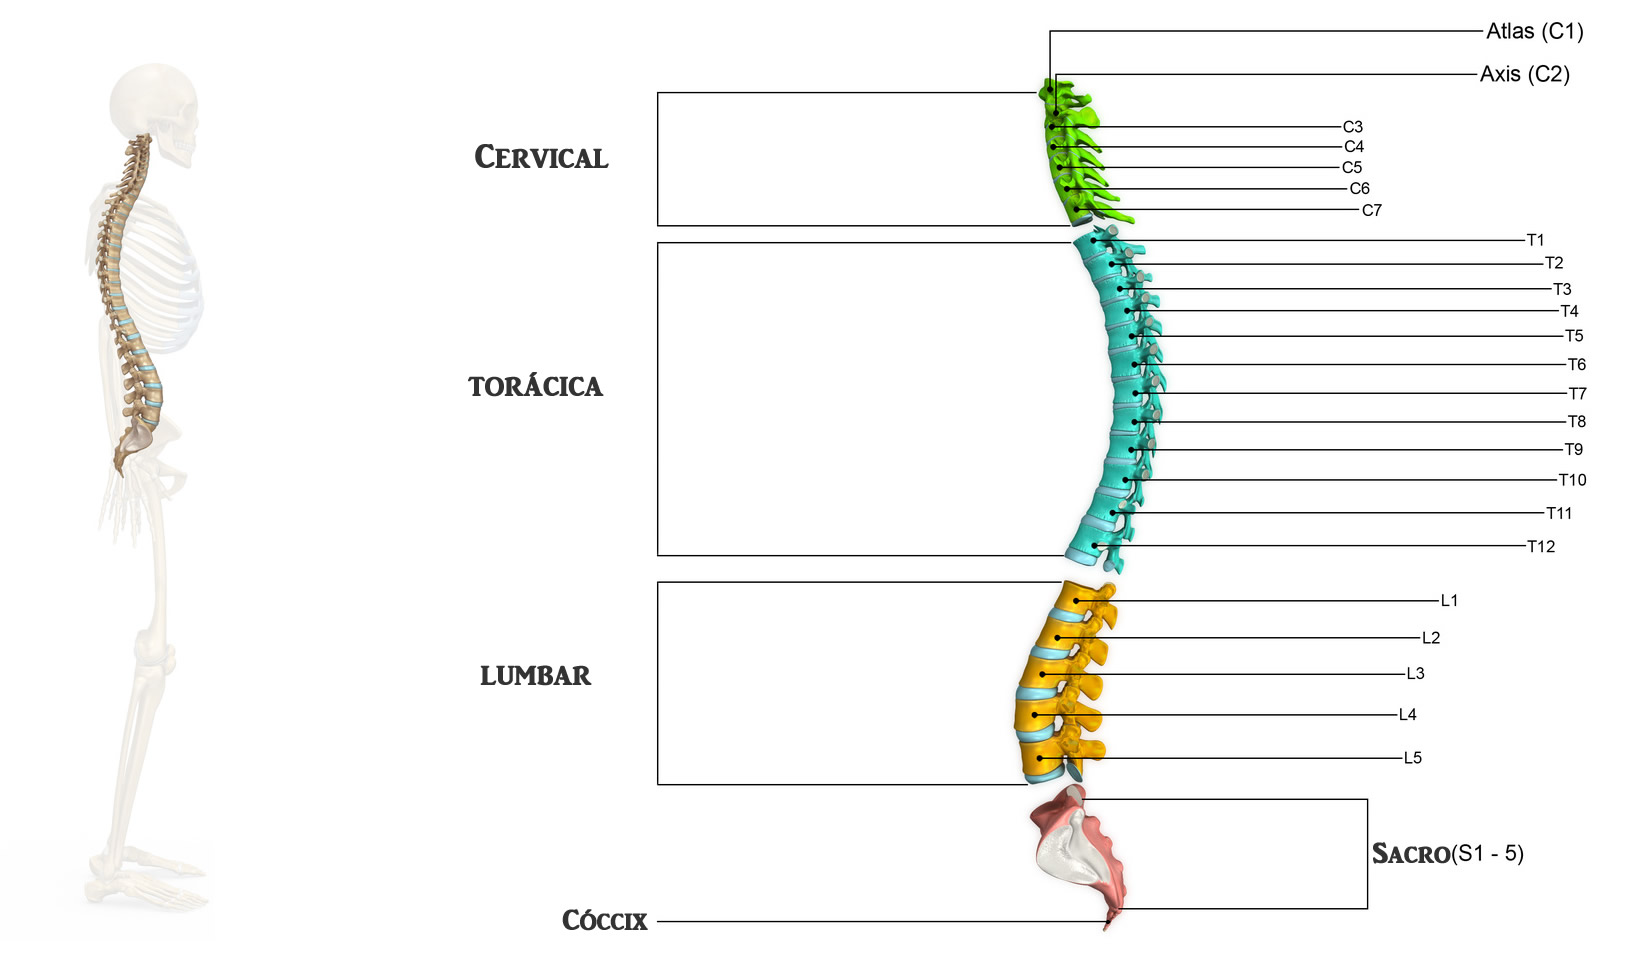
\includegraphics[scale=0.8]{columna_vertebral}
  \caption{Representación de la columna vertebral es sus 5 secciones\cite{columna_vertebral}.}\label{fig:columna_vertebral}
\end{figure}

Al igual que la columna vertebral, la médula espinal está organizada en 5 secciones de 31 segmentos en total: 8 cervicales, 12 torácicos, 5 lumbares, 5 sacrales y el nervio del coxis. Tiene una longitud total de entre 40 y 45 cm y cada segmento está asociado a dos nervios espinales, derecho e izquierdo. Este conjunto de nervios forman los nervios sensoriales, que entran en la médula espinal en cada segmento recibiendo información sensorial, y los nervios motores, que emergen de la misma y transmiten la información necesaria a los músculos para que éstos actúen en consecuencia.\cite{anatomia_medula_1}
\\
\\
Cada nervio espinal se compone de fibras nerviosas inervadas a miotomas (áreas musculares) y dermatomas (áreas de la piel)\cite{sci_clasificacion} siendo estos últimos fácilmente localizables en la superficie del cuerpo según se aprecia en la figura \ref{fig:dermatomas}\\

\begin{figure}[!htb]
\centering
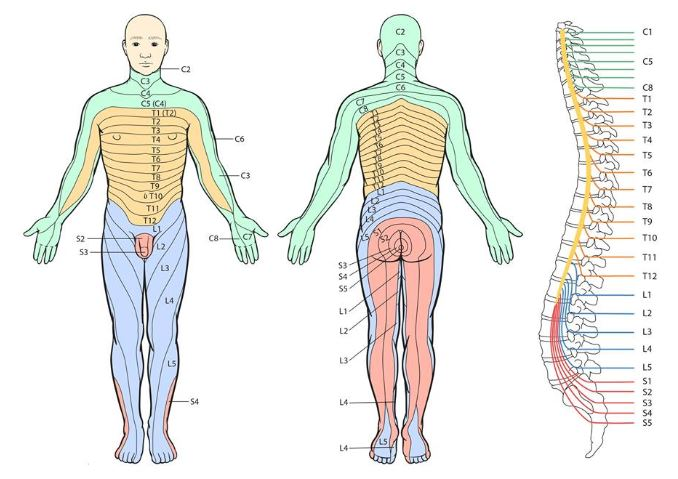
\includegraphics[scale=0.6]{dermatomas}
  \caption{Representación de dermatomas y su conexión con la médula espinal\cite{dermatomas}.}\label{fig:dermatomas}
\end{figure}


En lo que a miotomas o conjuntos de músculos se refiere, los segmentos cervicales están involucrados en la respiración y movimientos de cabeza, cuello y brazos. La sección torácica se encarga del control de dedos, pecho, espalda y abdomen. Por último, las secciones lumbar y sacral están asociadas con el control de músculos involucrados en la locomoción, micción, función intestinal y funciones reproductivas. 
\\
\\
Un análisis más profundo de la médula espinal conlleva estudiar su sección transversal. Esto revela un núcleo de materia gris en forma de mariposa o H rodeado de materia blanca. La materia gris está formada por neuronas motoras y sensoriales cada una con sus axones (prolongación de la neurona encargada de la transmisión de impulsos nerviosos) Por otra parte, la materia blanca está formada por fibras nerviosas que se conectan con diferentes áreas de la materia gris para transmitir impulsos nerviosos entre neuronas. De este modo, los axones de las neuronas sensoriales entran a la médula espinal (le transmiten información sensorial) mientras que los axones de las neuronas motoras salen de ésta (transmiten información motora a los músculos)\cite{sci_clasificacion}\cite{anatomia_medula_1}.
\\
\\
Tanto el tamaño de la sección como la proporción entre materia gris y blanca varía a lo largo de la médula espinal siendo mayor esta proporción en niveles inferiores ya que tienen menor cantidad de fibras nerviosas. De este modo, se distinguen 4 áreas en la sección de la médula espinal\cite{anatomia_medula_1}\cite{anatomia_medula_2}. La primera de ellas es el asta o cuerno dorsal que se encuentra en todos los niveles (cervical, torácico, lumbar, sacral y coxis) y está formado por núcleos sensoriales que reciben y procesan información sensorial. La columna intermedia y el cuerno o asta lateral están relacionados con órganos pélvicos y viscerales mediante neuronas del sistema nervioso autónomo o vegetativo. Por último, el cuerno o asta ventral está conectado a los músculos esqueléticos mediante neuronas motoras. Se aprecian los diferentes tipos de secciones a lo largo de la médula espinal en la figura \ref{fig:seccion_medula}\\

\begin{figure}[!htb]
\centering
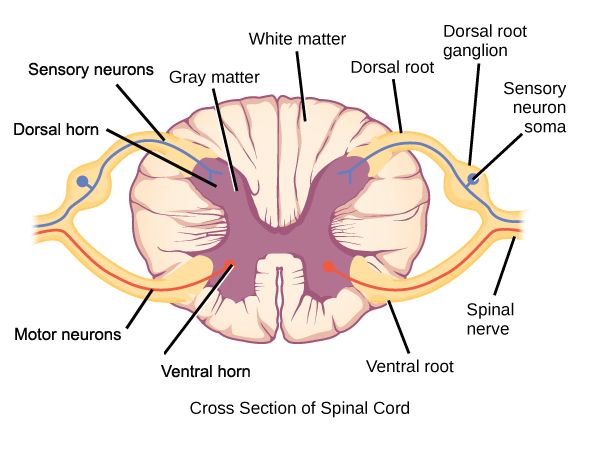
\includegraphics[scale=1.0]{seccion_medula}
  \caption{Sección transversal de médula espinal\cite{seccion_medula}.}\label{fig:seccion_medula}
\end{figure}


\section{Lesiones medulares}
Tras haber tratado los detalles pertinentes de la médula espinal, se procede a estudiar en este apartado el tipo de lesiones que esta puede sufrir y su clasificación según las consecuencias que producen en el paciente.

Una lesión en la médula espinal es cualquier tipo de alteración o anomalía que reduce o interrumpe la transmisión de impulsos nerviosos sensoriales y motrices con el cerebro por debajo del nivel en el que se produce dicha alteración\cite{sci_clasificacion}. Las causas más comunes de este tipo de lesiones son accidentes de tráfico, caídas, actos de violencia o agresiones, accidentes en deportes y actividades de recreación y enfermedades como cáncer, artritis y osteoporosis\cite{causas_sci}. Este tipo de lesiones no solamente producen pérdida de sensibilidad y movilidad sino que suponen una limitación considerable a la hora de realizar tareas esenciales en la vida diaria como vestirse, comer o asearse. Para un paciente con la médula espinal dañada, estas tareas pueden suponer en algunos casos una dificultad inconcebible requiriendo de asistencia externa.
\\
\\
No todas las lesiones de médula espinal son iguales ni suponen las mismas limitaciones, por lo que se va a proceder a la clasificación de las mismas así como los grados de independencia funcional en la realización de tareas esenciales en la vida diaria.


\subsection{Clasificación de lesiones medulares}\label{clasificacion_lesiones}
Para clasificar los tipos de daños en la médula espinal se deben examinar los dermatomas y miotomas para así poder determinar qué partes de la médula están afectadas. Pero antes de proceder a dicha clasificación se van a explicar ciertos términos para comprender mejor los tipos de lesiones en la médula espinal\cite{sci_clasificacion}:

\begin{itemize}
\item[•] \textbf{Tetraplejia:} Se refiere a la pérdida de funciones sensorial y/o motora en la zona cervical de la médula espinal. Afecta a brazos, tronco, piernas y órganos pélvicos.
\item[•] \textbf{Paraplejia:} Implica la pérdida de funciones sensorial y/o motora en las zonas torácica, lumbar o sacral. Se ven afectados tronco, piernas y órganos pélvicos.
\item[•] \textbf{Lesión incompleta:} Se conservan parcialmente las funciones sensoriales y/o motoras por debajo del nivel de la lesión.
\item[•] \textbf{Lesión completa:} Se produce cuando hay una pérdida total de funciones motora y sensoriales en el último segmento sacral de la médula.
\item[•] \textbf{Zona de preservación parcial:} Se refiere a todos aquellos dermatomas y miotomas que están parcialmente conectados a la médula.
\end{itemize}

Las lesiones de médula espinal se pueden clasificar según el estándar creado por la American Spinal Injury Association (ASIA)\cite{ASIA} y que se denomina como International Standards for Neurological and Functional Classification of Spinal Cord Injury. Para clasificar los daños en la médula espinal según este estándar, es necesario realizar un examen neurológico con dos componentes principales: sensorial y motriz. Además, cada componente tiene pruebas esenciales y opcionales que deben realizarse en el paciente. Los elementos esenciales generan una puntuación para determinar la clasificación de los daños en la médula mientras que los opcionales amplían la descripción clínica del paciente\cite{sci_clasificacion}.
\\
\\
El componente esencial del examen sensorial implica probar puntos clave de todos los dermatomas en ambos lados del cuerpo y que se pueden apreciar en la figura \ref{fig:dermatomas_clave}. En cada uno de estos puntos clave se examina la sensibilidad al toque ligero y a una sensación punzante. Se puntúa entonces la respuesta del paciente con un cero si no siente nada, uno si hay una apreciación ligera al estímulo y dos si la respuesta es normal. El componente opcional requiere un estímulo de presión o incluso dolor en cada punto clave de los dermatomas.\\

\begin{figure}[!htb]
\centering
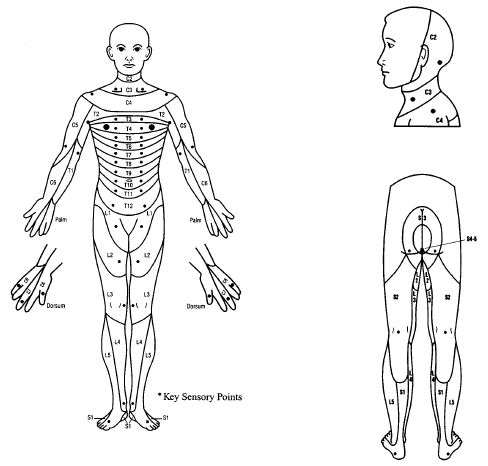
\includegraphics[scale=0.8]{dermatomas_clave}
  \caption{Puntos clave de cada dermatoma para su examen sensorial\cite{dermatomas_puntos}.}\label{fig:dermatomas_clave}
\end{figure}

En cuanto al examen motriz, su componente esencial implica probar un músculo clave de cada miotoma en ambos lados del cuerpo. Algunos de estos músculos son bíceps (flexión de codo) y tríceps (extensión de codo) para la sección cervical, abductores de dedos para la sección torácica, flexión de cadera para la sección lumbar y plantaflexores de tobillos para la sección sacral. Se mide a continuación la fuerza de dichos músculos generando cada uno de ellos una puntuación. Si no hay respuesta alguna del músculo, será puntuado con un cero. En cambio, si hay contracción visible pero sin movimiento la puntuación será de uno. Se valora con un dos un movimiento activo del músculo sin la acción de la gravedad y con un tres si es capaz de moverse en contra de ésta última. Por último, la puntuación será de cuatro si el músculo es capaz de moverse contra una resistencia moderada y de cinco si el movimiento es normal. El componente opcional de este examen implica probar músculos diferentes a los del componente esencial.
\\
\\
Una vez realizados los exámenes sensorial y motriz, se puede determinar el grado de la lesión que sufre la médula espinal. Éste caerá dentro de una de los puntos de la siguiente escala generada por el estándar de la ASIA mencionado previamente:

\begin{itemize}
\item[•] \textbf{Categoría A:} Lesión completa en los segmentos sacrales cuarto y quinto.
\item[•] \textbf{Categoría B:} Lesión incompleta con pérdida sensorial pero no motriz en los segmentos sacrales cuarto y quinto.
\item[•] \textbf{Categoría C:} Lesión incompleta en la que se preserva la función motriz. Además, por debajo del nivel de la lesión, más de la mitad de los músculos clave tienen una puntuación de menos de tres según el examen motriz mencionado previamente.
\item[•] \textbf{Categoría D:} Lesión incompleta en la que se preserva la función motriz. Además, por debajo del nivel de la lesión, más de la mitad de los músculos clave tienen una puntuación de tres o más según el examen motriz mencionado previamente.
\item[•] \textbf{Categoría E:} Funciones sensoriales y motrices normales.
\end{itemize}

Se recoge en la figura \ref{fig:estandar_asia} el estándar generado por la ASIA para la clasificación de lesiones en la médula espinal.\\

\begin{figure}[!htb]
\centering
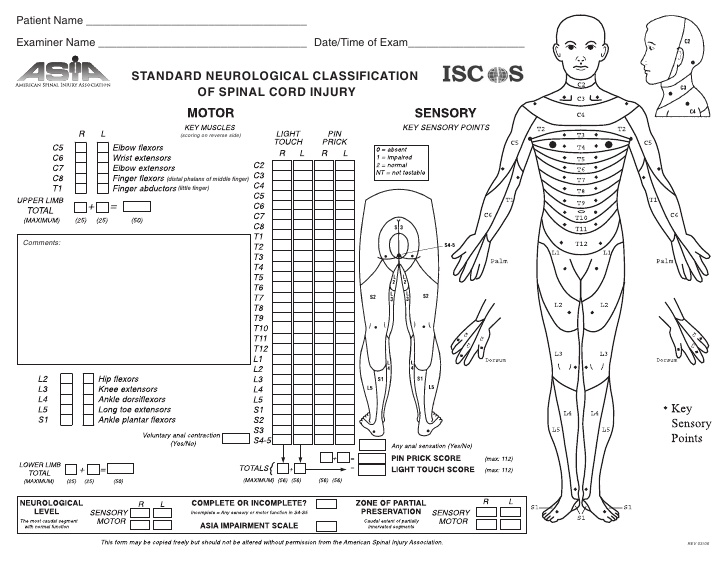
\includegraphics[scale=0.7]{estandar_asia}
  \caption{Plantilla del estándar para clasificación de lesiones en médula espinal\cite{estandar_asia}.}\label{fig:estandar_asia}
\end{figure}

\subsection{Clasificación de independencia funcional}
Además de la clasificación de lesiones de médula espinal, existe la Functional Independence Measure (FIM)\cite{sci_clasificacion} que sirve para determinar el grado de independencia funcional del paciente en la realización de diferentes tareas de la vida diaria. Este estándar se centra en seis áreas: cuidado personal, control de esfínter, movilidad, locomoción, comunicación e interacción social. Dentro de cada área, se evalúan dos o más actividades con un total de 18, como por ejemplo comer, asearse, bañarse o ducharse, vestirse la parte superior o inferior del cuerpo e ir al servicio. Cada tarea se evalúa según la siguiente escala diferenciando si el paciente es independiente o depende de supervisión o asistencia:

\begin{itemize}
\item[•] \textbf{7 puntos - Independencia completa:} La actividad es realizada de forma segura dentro de un tiempo razonable sin ningún tipo de ayuda.
\item[•] \textbf{6 puntos - Independencia modificada:} La actividad requiere la asistencia de algún dispositivo y/o no es realizada dentro de un tiempo razonable y/o no es llevada a cabo de forma segura.
\item[•] \textbf{5 puntos - Supervisión o uso de instalación:} No se requiere asistencia humana pero sí supervisión o algún tipo de soporte o instalación para facilitar la tarea.
\item[•] \textbf{4 puntos - Asistencia mínima:} El sujeto realiza el 75\% o más del esfuerzo requerido para la tarea. 
\item[•] \textbf{3 puntos - Asistencia humana moderada:} El sujeto realiza entre el 50\% y 75\% del esfuerzo requerido para la tarea.
\item[•] \textbf{2 puntos - asistencia máxima:} El sujeto realiza entre el 25\% y 50\% del esfuerzo requerido para la tarea.
\item[•] \textbf{1 punto - Asistencia total:} El sujeto realiza entre el 0\% y 25\% del esfuerzo requerido para la tarea.
\end{itemize}

Por lo tanto, la puntuación total del examen FIM (suma de la puntuación de cada tarea) estima el grado de discapacidad en términos de seguridad y dependencia humana o de algún dispositivo. Con este examen se determina con exactitud qué áreas y tareas de la vida diaria están más afectadas a causa de la lesión en la médula espinal. 


%Se aprecia en la figura \ref{fig:examen_fim} la plantilla para la realización del examen FIM.

%\begin{figure}[!htb]
%\centering
%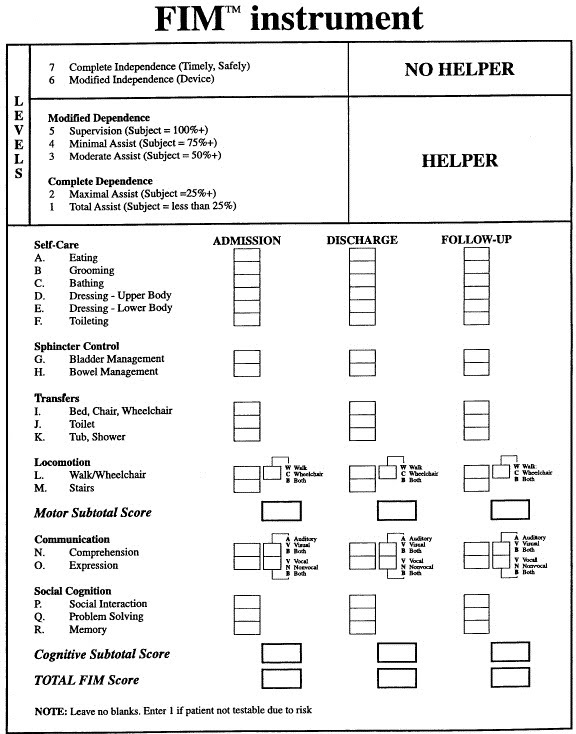
\includegraphics[scale=0.5]{examen_fim}
%  \caption{Plantilla del estándar para clasificación de %independencia funcional\cite{examen_fim}.}\label{fig:examen_fim}
%\end{figure}


\section{Rehabilitación de lesiones en el sistema nervioso central}
A pesar de la gravedad e impacto fisiológico y psicológico que supone una lesión en el sistema nervioso central ya sea procedente de ictus o daño medular, es importante tener en cuenta que sus efectos pueden mitigarse enormemente si se lleva a cabo un proceso adecuado de rehabilitación.
\\
\\
La rehabilitación de este tipo de lesiones entra en el marco de la terapia ocupacional, un tratamiento especializado que ayuda a los pacientes a incrementar su independencia en numerosos aspectos de su vida. Esta terapia permite desarrollar a los pacientes las habilidades necesarias del día a día y así conseguir un nivel de vida satisfactorio e independiente. La terapia ocupacional en el ámbito de la rehabilitación de lesiones en el sistema nervioso central se basa en la adaptación social del paciente y recuperación de habilidades. De forma adicional, se trata de alcanzar ciertos objetivos individuales que son específicos de cada paciente\cite{rehabilitacion}.
\\
\\
Un paciente que sufre una lesión en la médula espinal puede mostrarse desanimado con su terapia cuando sus logros son pocos y distantes en el tiempo. Es por esto por lo que es bueno realizar una gran variedad de actividades adaptadas a cada paciente. De este modo, se impulsa su autoestima resaltando las habilidades funcionales que posee y ya sean físicas, sociales, emocionales, sensoriales o cognitivas. Por lo tanto, la contribución de la terapia ocupacional al rendimiento de los pacientes reside en la realización de actividades útiles para promover su salud física, psicológica e incrementar su independencia funcional.
\\
\\
Es importante que la terapia ocupacional comience lo antes posible tras la estabilización del paciente después de sufrir la lesión. De esta forma, se pueden trabajar con de forma efectiva los siguientes puntos:

\begin{itemize}
\item[•] Evaluar las habilidades y rendimiento del paciente en su hogar, trabajo y tiempo libre.
\item[•] Proporcionar terapia individual para desarrollar actividades de la vida diaria mediante diferentes técnicas.
\item[•] Facilitar técnicas que ayuden al paciente a salvar los efectos de la lesión.
\item[•] Implementar ejercicios y rutinas que ayuden a fortalecer los músculos que hayan podido ser afectados por la lesión.
\item[•] Determinar el tipo de dispositivos de asistencia para otorgar al paciente más independencia en la realización de tareas.
\end{itemize}


Para una correcta realización de la terapia, ésta debe llevarse a cabo en centros especializados con un equipo interdisciplinar de profesionales y un seguimiento riguroso del estado del paciente.
\\
\\
El proceso de rehabilitación se compone tradicionalmente por tres fases: aguda, sentada y sub-aguda. En la fase aguda se efectúan actividades fisioterapéuticas tanto por encima como por debajo del nivel de la lesión para evitar atrofia y mantener en forma los músculos así como un movimiento natural en las articulaciones. Tras esta fase, comienzan los ejercicios para que el paciente consiga, de forma progresiva, incorporarse sobre la cama y sentarse en ésta evitando así reacciones neurovegetativas como consecuencia de la lesión. Por último, comienza la fase sub-aguda en la que se realizan todo tipo de actividades terapéuticas dependiendo del tipo de lesión y de las características del paciente (edad, peso, motivación etc.) De este modo, se incrementan la independencia y habilidades funcionales ya descritas con anterioridad. Hay que tener en cuenta que cada paciente le dará una importancia relativa a cada actividad de modo que éstas se adaptan en consecuencia\cite{tesis_antonio}\cite{etapas_rehabilitacion}.


\subsection{Neuro-rehabilitación de la marcha patológica}
La habilidad del ser humano para caminar está integrada en el sistema nervioso central siendo su principal componente el conjunto de conexiones interneuronales inherentes a la médula espinal. Dichas conexiones se denominan Generadores Centrales de Patrones (GCP) ya que generan el patrón adecuado de activación de los músculos involucrados para caminar. Estos patrones dependen de determinadas entradas sensoriales como la visión y los sistemas vestibular (sentido de movimiento y equilibrio) y propioceptivo (percepción de posición y movimiento del cuerpo) Por lo tanto, el propósito de la tarea que implica caminar es esculpir los patrones de activación de músculos, controlar la transición entre fases del paso y reforzar los resultados satisfactorios\cite{rehabilitacion_caminar}.
\\
\\
Un correcto funcionamiento del sistema nervioso central a la hora de activar los músculos correctamente tal y como se ha mencionado con anterioridad, resulta en la marcha del ser humano. Se trata de un proceso de locomoción en el que el cuerpo se mueve hacia adelante soportando su peso de forma alternativa por ambas piernas. Puesto que es un proceso repetitivo, se puede explicar mediante el ciclo de la marcha recogido en la figura \ref{fig:ciclo_marcha}. El ciclo comienza en el momento en que uno de los pies entra en contacto con el suelo mediante el talón. De este modo, comienza la fase de apoyo que se divide a su vez en dos sub-fases: asimilación del peso y apoyo sobre un miembro. La primera se encarga de estabilizar el miembro absorbiendo el golpe y conservar la inercia del cuerpo mientras que la segunda ofrece un punto de apoyo y estabilidad al cuerpo mientras avanza. Para terminar el ciclo, se entra en la fase de balanceo que comienza con la transición entre la fase anterior y actual levantando el pie del suelo. A continuación, las sub-fases de balanceo inicial, medio y terminal describen la trayectoria de la pierna hasta que vuelve a apoyarse en el suelo y pone fin a una repetición del ciclo de marcha\cite{ciclo_marcha}.\\

\begin{figure}[!htb]
\centering
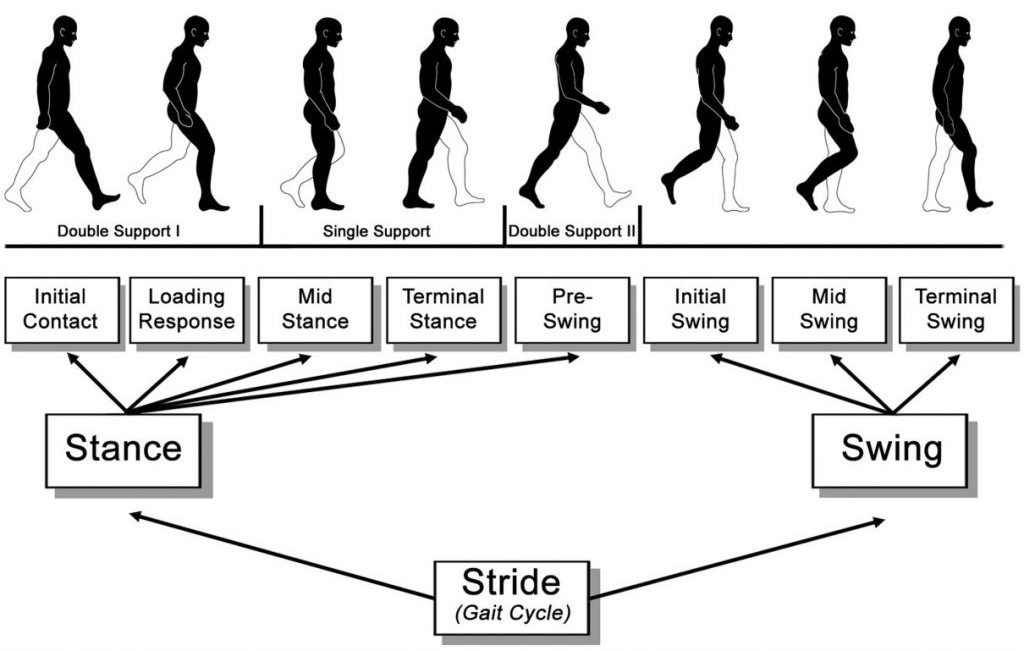
\includegraphics[scale=0.5]{ciclo_marcha}
  \caption{Ciclo de marcha en el ser humano\cite{ciclo_marcha}.}\label{fig:ciclo_marcha}
\end{figure}

Un factor importante en el ciclo de la marcha es la fuerza muscular, pues entrenarla conduce a hipertrofia y una mejor coordinación entre músculos. Sin embargo, incrementar la fuerza muscular no implica mejorar la locomoción y viceversa\cite{recovery_locomotion}. 
\\
\\
Por tanto, la neuro-rehabilitación de la marcha patológica está enfocada a mejorar las habilidades de locomoción del paciente haciendo énfasis en los músculos por debajo del nivel de la lesión. De este modo, las zonas de la médula espinal encargadas de la locomoción pueden ser activadas proporcionando los estímulos adecuados. Esto es posible en el caso de lesiones incompletas ya que para las lesiones completas no se habla de neuro-rehabilitación sino de compensación. En este caso, se pretende conseguir el reaprendizaje de funciones motrices con la ayuda de dispositivos externos. El resultado dependerá de la presencia de circuitos interneruonales capaces de generar patrones de movimiento\cite{recovery_locomotion}.

\subsection{Tecnologías para la neuro-rehabilitación de la marcha patológica}
El proceso de neuro-rehabilitación de la marcha patológica es llevado a cabo por profesionales encargados de ejercitar a los pacientes. Aunque el movimiento en las articulaciones y demás ejercicios es natural y controlado por el terapeuta, se puede perder la consistencia tras largas sesiones y son necesarios varios terapeutas debido al cansancio acumulado, lo cual afecta a la terapia. Por lo tanto, junto a estos métodos de neuro-rehabilitación tradicionales y que son insustituibles, se tienen tecnologías adicionales que favorecen la terapia: entrenamiento robótico del paso y electroestimulación, tecnologías utilizadas en el desarrollo de la prótesis híbrida y en el que está centrado el presente trabajo fin de máster. Se expone a continuación la relación de estas tecnologías con la neuro-rehabilitación de lesiones medulares e ictus dirigida a la marcha patológica.

\subsubsection{Asistencia robótica}

La robótica supone una herramienta de gran valor en la neuro-rehabilitación gracias al uso de exoesqueletos robóticos que pueden definirse como \textit{dispositivos electromecánicos desarrollados para la aumentación de las capacidades físicas del portador o como dispositivo ortopédico para la neuro-rehabilitación de la locomoción o ciclo de marcha}\cite{exoesqueletos}. 
\\
\\
Existen dos tipos principales de exoesqueletos: rígidos y flexibles. El primer tipo, como su nombre indica, implica la utilización de elementos y materiales rígidos para la estructura y fijación del exoesqueleto al paciente. En el segundo caso, se utilizan materiales no rígidos como pueden ser diferentes tipos de textiles. La principal desventaja de un exoesqueleto flexible reside en su alcance en el sentido de su limitada capacidad de aportar fuerza, par y velocidad sobre los miembros del paciente. Esto es una consecuencia inherente al uso de materiales flexibles. Por lo tanto, se usan principalmente cuando se requieren bajos niveles de asistencia o cuando el paciente no tiene dañados los huesos o las articulaciones. Por otra parte, los exoesqueletos rígidos son capaces de proporcionar mayor fuerza, par y velocidad además de hacerlo de forma más precisa para producir movimiento incluso en los casos de parálisis extrema en el paciente. En cuanto a los materiales utilizados, se desea un equilibrio entre integridad estructural y peso de modo que se emplea acero, aluminio, fibra de carbono o piezas impresas en 3D con filamentos de polímeros termoplásticos acrilonitrilo butadieno estireno (ABS) y ácido poliláctico (PLA).\cite{estudio_exoesqueletos}\cite{comparacion_exoesqueletos}. Se pueden apreciar ejemplos de ambos tipos de exoesqueletos en la figuras \ref{fig:exoesqueleto_rigido} y \ref{fig:exoesqueleto_flexible}.\\

\begin{figure}[!htb]
\minipage{0.35\textwidth}

  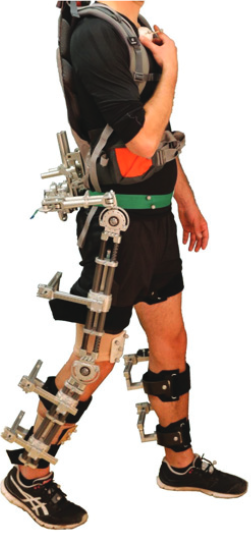
\includegraphics[width=\linewidth]{exoesqueleto_rigido}
  \caption{Exoesqueleto rígido para neuro-rehabilitación de marcha patológica\cite{exoesqueleto_rigido}}\label{fig:exoesqueleto_rigido}
\endminipage\hfill
\minipage{0.55\textwidth}%
  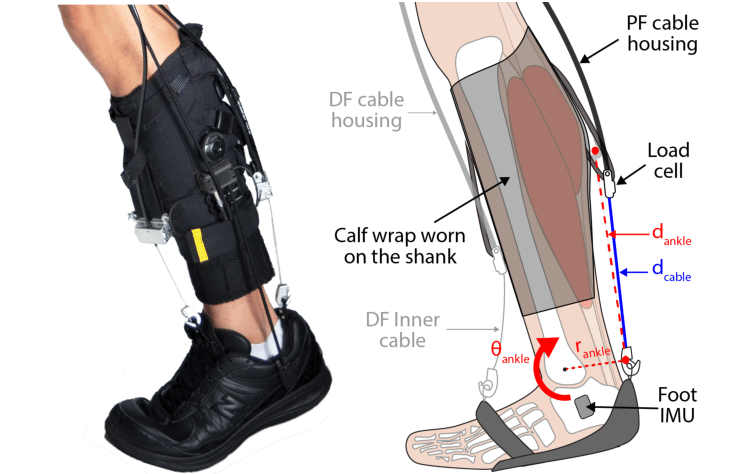
\includegraphics[width=\linewidth]{exoesqueleto_flexible}
  \caption{Exoesqueleto flexible para el control del movimiento del tobillo\cite{exoesqueleto_flexible}}\label{fig:exoesqueleto_flexible}
\endminipage

\end{figure}

Los exoesqueletos disponen de diferentes tipos de actuadores para generar movimiento. Se describen a continuación algunos de los más comunes y que además forman parte del exoesqueleto utilizado en la prótesis híbrida\cite{estudio_exoesqueletos}\cite{tesis_antonio}\cite{actuadores_exoesqueletos}:

\begin{itemize}
\item[•]\textbf{Motores de corriente continua:} Es el tipo de actuador más usado en exoesqueletos ya que es fácil de controlar y ofrece respuestas rápidas y un par elevado para manejar las partes más pesadas del exoesqueleto. Según la aplicación y el tipo de control requerido se usan estos motores de forma directa o con una reductora si lo que se pretende es un movimiento rápido y fuerte o lento y controlado, respectivamente. Además, se usan motores con escobillas si se desea prescindir de electrónica o bien motores sin escobillas si lo que se desea es un mejor ratio potencia/peso.

\item[•]\textbf{Almacenamiento de energía elástica:} Se trata de todo tipo de dispositivo, como resortes o muelles, capaz de almacenar energía elástica durante determinadas fases del ciclo de marcha para liberarla después en otras fases. Es un método robusto y que no requiere de fuentes de energía pero no se puede tener un control preciso sobre la respuesta que ofrecen estos actuadores.

\item[•]\textbf{Accionamientos hidráulicos:} Es el actuador con el mejor ratio par/peso ya que puede generar valores muy elevados de fuerza. Esto se debe a la inyección de un fluido a alta presión, como puede ser aceite, dentro de un cilindro para producir movimiento en un émbolo sujeto a la prótesis. Sin embargo, su principal desventaja implica la necesidad de una bomba junto a un depósito de aceite lo que supone problemas de ruido y fugas además de un control no lineal del movimiento.

\item[•]\textbf{Accionamientos neumáticos:} Al igual que los actuadores hidráulicos, poseen un gran ratio fuerza/peso, en este caso debido a la inyección de aire a alta presión del mismo modo que en el actuador anterior. Aunque es más ligero que éste y produce movimientos más naturales acorde a un comportamiento muscular normal, también sufre problemas de fugas, ruido y movimiento no lineal.




%\item[•]\textbf{Motores ultrasónicos:} Su funcionamiento se basa en el fenómeno piezoeléctrico, es decir, el estator recibe energía eléctrica y la tranforma en vibraciones mecánicas que pasan al rotor, elemento que transforma esas vibraciones en movimiento circular mediante fricción. Esto es posible debido a los materiales piezoeléctricos que conectan estator y rotor. su principal ventaja es que pueden llegar a tener un ratio par/volumen hasta 20 veces superior al de los motores de corriente continua. Además de ser ligero y compacto, no produce ruido y puede operar a muy baja velocidad con gran precisión. Sin embargo, son muy difíciles de fabricar y por lo tanto una carga económica importante.

%\item[•]\textbf{Aleaciones de memoria de forma:} Son aleaciones metálicas, principalmente de cobre, aluminio y níquel que, ante una deformación plástica, son capaces de recuperar su forma anterior a ésta si alcanzan cierta temperatura debido a cambios en la estructura cristalina de la aleación. Estos actuadores pueden proporcionar grandes fuerzas y desplazamientos con un buen ratio potencia/peso. Sin embargo, se debe tener en cuenta que su actuación no es simétrica ya que los movimientos de contracción son generalmente más rápidos que los de elongación, lo que dificulta su control.


%\item[•]\textbf{Polímeros electroactivos:} Es un tipo de material elástico desarrollado recientemente y cuyas características son muy similares a las del músculo humano. El movimiento en este tipo de material se produce al ser estimulado con campos eléctricos. Presenta un alto rango de potencia además de una conversión de energía eléctrica a mecánica altamente eficiente. Sin embargo, tiene un ratio par/peso reducido por lo que de momento no es un material óptimo para exoesqueletos de modo que es necesaria más investigación para mejorar sus propiedades.
\end{itemize}


Teniendo en cuenta las características y capacidades de los exoesqueletos, si se emplean como herramientas de neuro-rehabilitación, es posible replicar los ejercicios que el terapeuta efectúa sobre el paciente con diferentes configuraciones de fuerza, par y velocidad. Además, se pueden llevar a cabo ejercicios que son imposibles para un terapeuta debido a limitaciones de fuerza, repetibilidad o sensibilidad\cite{robotica_rehabilitacion}.
\\
\\
Debido a la utilidad y versatilidad del uso de la robótica en forma de exoesqueleto en la neuro-rehabilitación, surge el concepto de assist-as-needed (AAN)\cite{assist_as_need} y que implica la asistencia y corrección de los movimientos del paciente. De este modo, el paciente trata de efectuar un ejercicio mientras que el robot le proporciona asistencia solamente cuando la necesita. El nivel de asistencia varía en función de la desviación del paciente respecto a la trayectoria planteada por el ejercicio por lo que un exoesqueleto robótico tiene en este campo un gran alcance ya que puede administrar varios patrones motrices y sensoriales. El hecho de aportar esta variabilidad motriz y sensorial potencia la habilidad de aprendizaje de la médula espinal evitando las incongruencias procedentes de un patrón fijo de movimientos para caminar.
\\
\\
Una de las ventajas del uso de exoesqueletos en neuro-rehabilitación de marcha patológica es su mayor seguridad y control sobre el ejercicio respecto a la terapia tradicional. Además, no solo permiten rehabilitar el ciclo de marcha sino que potencian las capacidades físicas del paciente si se sigue usando esta herramienta mucho después del momento en que se produjo la lesión. Es importante considerar también el factor de motivación del paciente puesto que un exoesqueleto ayuda a conseguir resultados de forma más rápida y efectiva mejorando así la velocidad y eficiencia de la neuro-rehabilitación. Por otra parte, es importante considerar que dos tercios de los pacientes con lesiones medulares sufren de sobrepeso u obesidad debido a la falta de ejercicio físico. En este aspecto, un exoesqueleto ayuda a combatir el sobrepeso ya que reduce el tiempo requerido para realizar los ejercicios de neuro-rehabilitación, aumenta la cantidad de actividad física realizada por el paciente y ayuda a mejorar la composición de determinadas partes del cuerpo. Sin embargo, la mayoría de los exoesqueletos disponibles son capaces de soportar pacientes de hasta 100 Kg lo que deja fuera de esta terapia a un número considerable de sujetos\cite{ventajas_desventajas_exoesqueletos}. 
\\
\\
Por último, desde un punto de vista más técnico, clínico y económico, un exoesqueleto está formado por una estructura compuesta de diferentes tipos de materiales como acero, aluminio, fibra de carbono, textiles adecuados así como actuadores ya descritos. Esto supone un conjunto de elementos no asequible para cualquier individuo o institución. Además, se trata de una herramienta generalmente aparatosa y/o pesada por lo que su uso queda principalmente reducido a un ambiente clínico y no a la vida diaria del paciente en su hogar, trabajo u otras áreas.
\\
\\
Para terminar, uno de los dispositivos más utilizados en la neuro-rehabilitación del ciclo de marcha en ambientes clínicos es el Lokomat\cite{lokomat}. Está formado por una prótesis robótica especializada para caminar junto a un sistema de soporte del peso corporal y una cinta. Dispone de 4 grados de libertad mediante movimientos lineales: articulaciones derecha e izquierda de cadera y rodillas. Las piernas del paciente están sujetas por la prótesis y lo movimientos lineales de la misma sincronizados con la velocidad de la cinta de caminar. El concepto de AAN entra en juego en el Lokomat permitiendo al paciente moverse libremente dentro de un espacio designado para el patrón del paso. Se consigue por tanto más variabilidad y libertad de movimiento y adaptación del paso para cada paciente que siguiendo la neuro-rehabilitación tradicional. Se muestra en la figura \ref{fig:lokomat} el dispositivo descrito.\\

\begin{figure}[!htb]
\centering
\minipage{0.6\textwidth}
  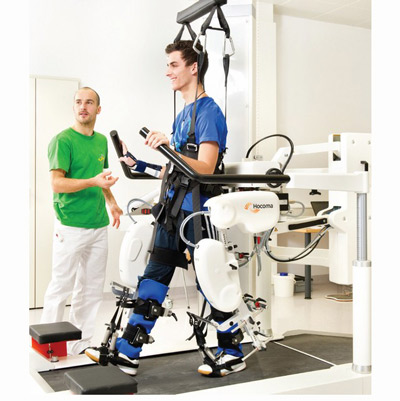
\includegraphics[width=\linewidth]{lokomat}
  \caption{Dispositivo Lokomat para neuro-rehabilitación de la marcha patológica\cite{lokomat_imagen}.}\label{fig:lokomat}
\endminipage\hfill
\end{figure}

\subsubsection{Asistencia por electroestimulación mediante neuroprótesis}

Una alternativa para trabajar sobre los músculos del paciente es la electroestimulación o estimulación eléctrica de los tejidos neuromusculares. Con una configuración adecuada se pueden estimular músculos paralizados tras la lesión medular para permitir caminar al paciente y llevar a cabo la neuro-rehabilitación\cite{electroestimulacion2}.
\\
\\
Es preciso diferenciar entre electroestimulación muscular, del inglés Muscle Electrical Stimulation (MES) o simplemente electroestimulación y electroestimulación funcional, es decir Functional Electrical Stimulation (FES). La primera implica la tranmisión de pulsos eléctricos a los músculos para conseguir su estimulación en forma de contracción muscular con diferentes fines como puede ser el entrenamiento deportivo\cite{sanitas}. La segunda consigue emparejar la estimulación de forma simultánea o intermitente con una determinada tarea o ejercicio, por ejemplo, caminar o realizar ciertos movimientos con las extremidades. Esto consitutuye una neuroprótesis motora o NeuroProsthesis (NP)\cite{tesis_antonio}.
\\
\\
En su forma más básica, la electroestimulación es la interacción mediante señales eléctricas con partes del cuerpo que conservan respuesta a dicho estímulo. De este modo, aplicando pequeños pulsos eléctricos sobre músculos o nervios se puede producir su contracción y por lo tanto estimulación y movimiento artificial en el cuerpo. Sin embargo, el resultado final depende de cada patología y caso del paciente así como la efectividad con la que se lleva a cabo la electroestimulación y que involucra el tipo de electrodos utilizados, su colocación, selectividad de músculos, impedancia de la piel, integridad muscular etc. \cite{electroestimulacion}.
\\
\\
Para la aplicación de corriente existen diferentes tipos de electrodos: superficiales (parches sobre la piel), transcutáneos (aguja con un cable por dentro para atravesar la piel y contactar con el músculo o nervio) o implantados (permanentemente fijados a los nervios para largo uso siempre que sea biocompatible en el paciente)\cite{tipos_electrodos}
Una vez seleccionado el tipo de electrodos, se colocan dos por cada músculo o nervio de modo que uno sirve como cátodo y otro como ánodo. Es importante colocar los electrodos correctamente, es decir, sobre puntos motrices de los músculos y nervios, así como conseguir una selectividad adecuada. Éste último término hace referencia a la estimulación de los músculos y nervios deseados con la intensidad adecuada para evitar efectos adversos\cite{limitaciones_fes}. Se aprecia en las figuras \ref{fig:electrodo_superficial} y \ref{fig:electrodo_percutaneo} algunos de los diferentes tipos de electrodos usados en electroestimulación.\\

\begin{figure}[!htb]
\minipage{0.45\textwidth}
  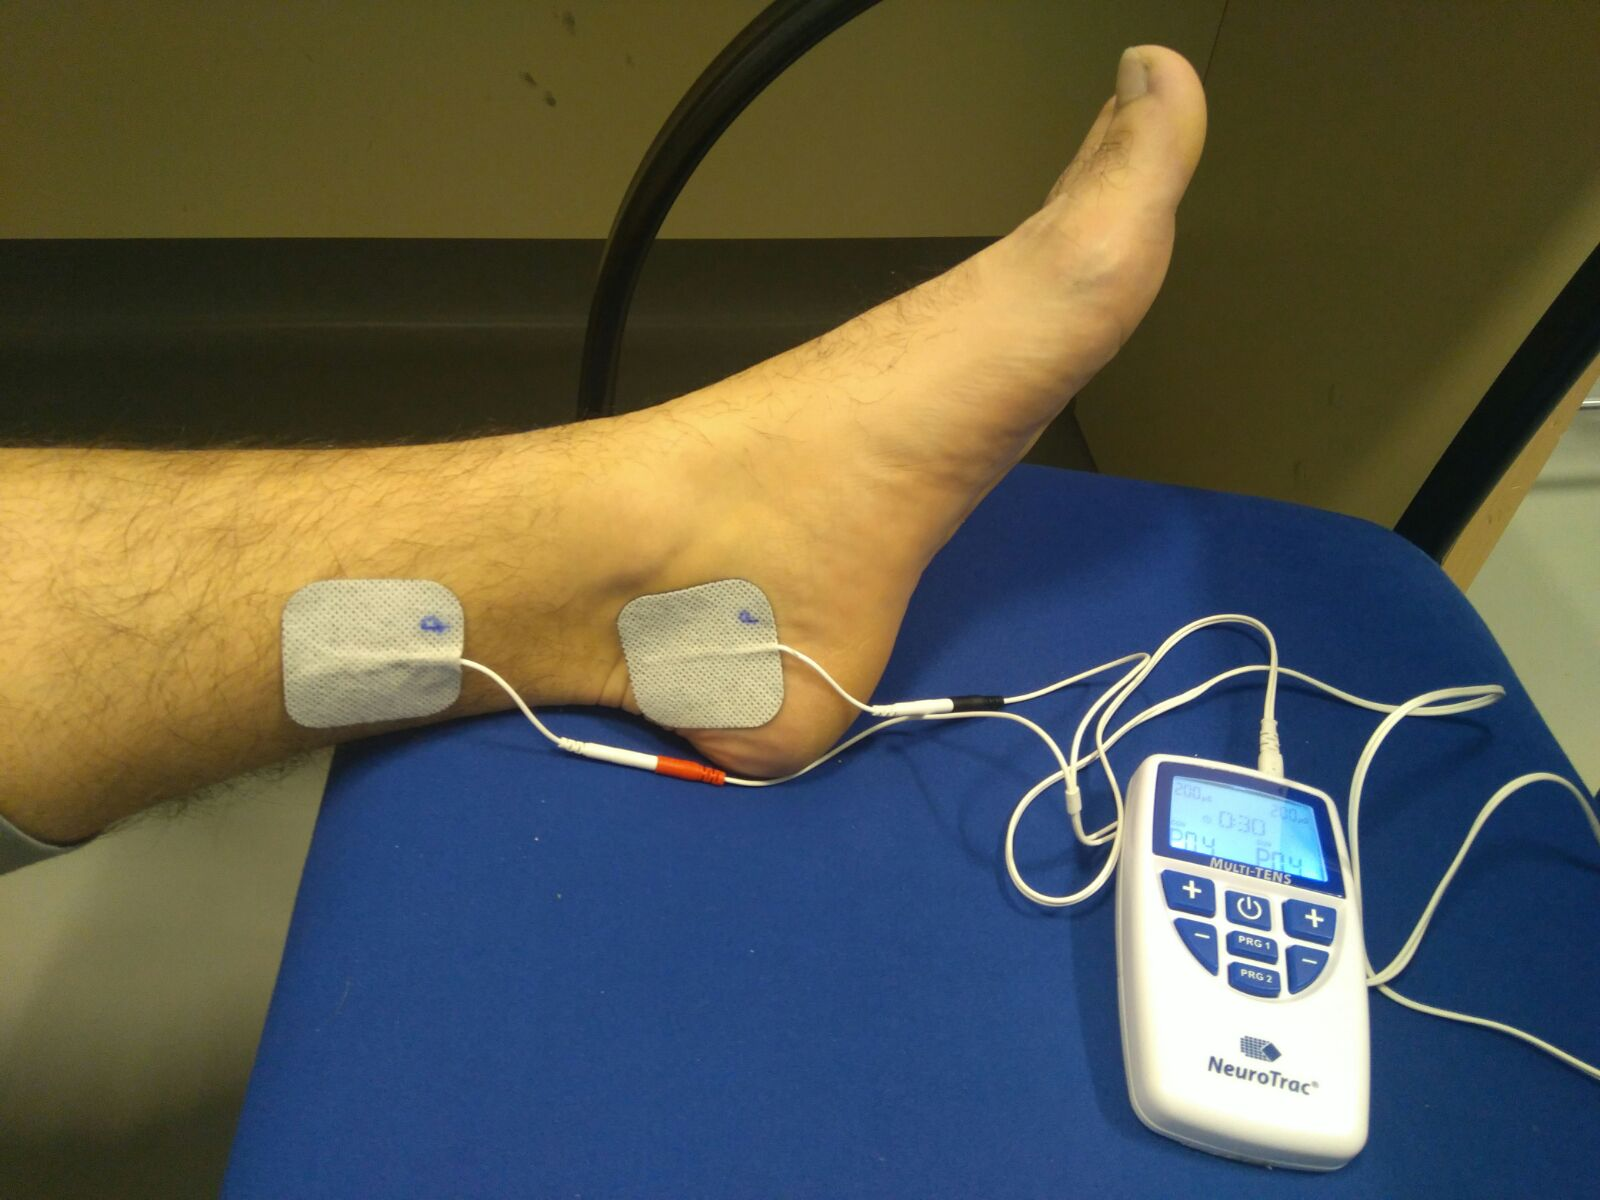
\includegraphics[width=\linewidth]{electrodo_superficial}
  \caption{Electrodo superficial\cite{electrodo_superficial}.}\label{fig:electrodo_superficial}
\endminipage\hfill
\minipage{0.45\textwidth}
  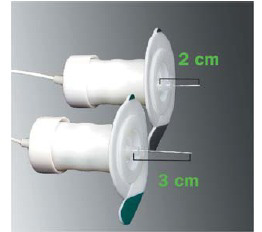
\includegraphics[width=\linewidth]{electrodo_percutaneo}
  \caption{Electrodo percutáneo\cite{electrodo_percutaneo}.}\label{fig:electrodo_percutaneo}
\endminipage\hfill
\end{figure}

La aplicación de estímulos eléctricos puede llevarse a cabo mediante pulsos de tensión o de corriente. Usar pulsos de tensión implica que el daño producido sobre los tejidos del cuerpo viene dado por el valor de densidad de corriente, lo que influye en la respuesta muscular de modo que si existe una alta impedancia entre le electrodo y el músculo, la corriente que llega al mismo para un determinado valor de tensión será menor. Por otro lado, utilizar pulsos de corriente imita mejor los movimientos naturales del cuerpo y muestra resultados más consistentes y repetibles así como menor variación en la impedancia de la piel y otros tejidos. Por lo tanto, una configuración óptima evita que la impedancia varíe a lo largo del proceso y por tanto afecte a la corriente que llega al músculo, cuya respuesta depende directamente de ésta\cite{FES}. Por ello, es preferible utilizar pulsos de corriente en vez de pulsos de tensión y para lo que es necesario utilizar una fuente de corriente adecuada, dispositivo que se explicará más adelante.
\\
\\
Los parámetros de un pulso de corriente son amplitud, ancho de pulso, periodo inter e intra pulso y forma del pulso\cite{parametros_FES}. La forma del pulso determina cómo se va a aplicar corriente entre los electrodos generando diferentes patrones de pulsos de corriente. Algunos de estos patrones se explican a continuación\cite{FES} y pueden apreciarse en la figura \ref{fig:patrones_pulsos}:

\begin{itemize}
\item[•] \textbf{Pulso monofásico:} Se aplica corriente en un solo sentido, es decir, de ánodo a cátodo o de cátodo a ánodo. Produce daño en tejidos y deterioro del electrodo por su efecto polarizante al alterar la distribución iónica de la zona de aplicación.
\item[•] \textbf{Pulso bifásico asimétrico:} Se aplica una corriente en un sentido y después otra diferente en el otro. Al ser bidireccional permite a los iones circular en dos sentidos minimizando la redistribución de éstos y el daño en tejidos y electrodos.
\item[•] \textbf{Pulso bifásico simétrico:} Se aplica corriente primero en un sentido y después ese mismo valor de corriente en el otro. Se consigue neutralizar el efecto polarizante pero la corriente anódica puede suprimir parte de la corriente catódica y viceversa. Por tanto, los pulsos anódicos y catódicos se distancian en el tiempo para evitar el mencionado efecto.
\end{itemize}

\begin{figure}[!htb]
\centering
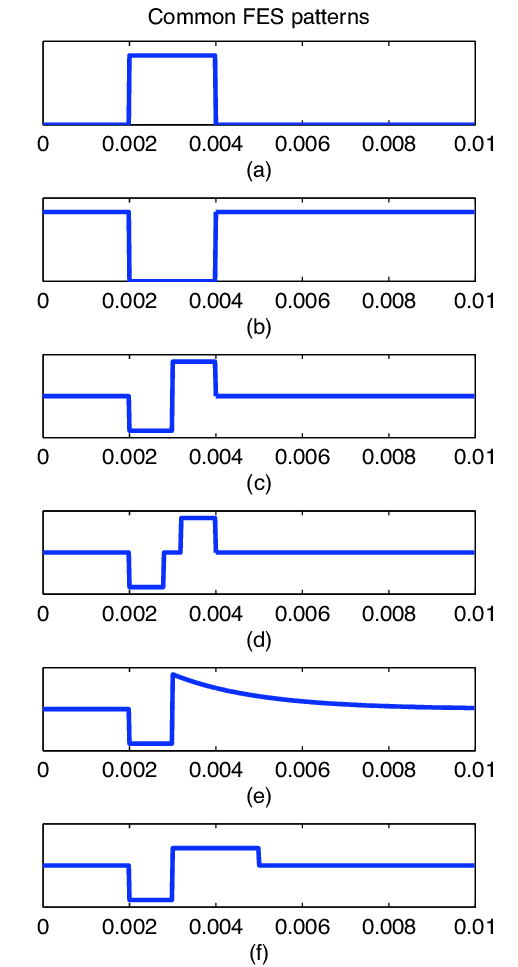
\includegraphics[scale=0.3]{patrones_pulsos}
  \caption{Patrones de pulsos de corriente\cite{FES}. Pulso monofásico (a) y (b), pulso bifásico simétrico sin espaciado (c) y con espaciado temporal (d) y pulsos bifásicos asimétricos (e) y (f). Se aprecia que el pulso (e) tiene una rampa para que la estimulación sea más natural y suave.}\label{fig:patrones_pulsos}
\end{figure}

Una vez expuestos algunos de los posibles patrones de pulsos, la amplitud es la intensidad de corriente ($mA$) aplicada de ánodo a cátodo o de cátodo a ánodo durante el tiempo especificado por el ancho de pulso (del orden de $us$ y $ms$). El periodo intra pulso es el tiempo que separa la aplicación de corriente positiva y negativa en un pulso bifásico. Por último, es necesario indicar que la electroestimulación se efectúa mediante trenes de pulsos, es decir, repeticiones de pulsos hasta conseguir el efecto deseado en los músculos. El periodo de repetición de pulsos está determinado por el periodo inter pulso y según su configuración da lugar a diferentes tipos de trenes de pulsos\cite{tipos_repeticion} mostrados en la figura \ref{fig:tipos_repeticion}:


\begin{itemize}
\item[•] \textbf{Tren de frecuencia constante:} Implica la repetición de un pulso de corriente a frecuencia constante. 
\item[•] \textbf{Tren de frecuencia variable:} Se comienza el tren con dos pulsos próximos en el tiempo y se sigue con una repetición constante de pulsos simples.
\item[•] \textbf{Tren de pulsos dobles:} Se repiten a frecuencia constante dos pulsos próximos en el tiempo. 
\end{itemize}

El motivo por el que se utilizan pulsos dobles es para aprovechar el efecto muscular en forma de un incremento de fuerza considerable ante estímulos de alta frecuencia (dos pulsos de corriente seguidos) Se utiliza de forma limitada porque produce fatiga en el músculo\cite{catch_like}.\\

\begin{figure}[!htb]
\centering
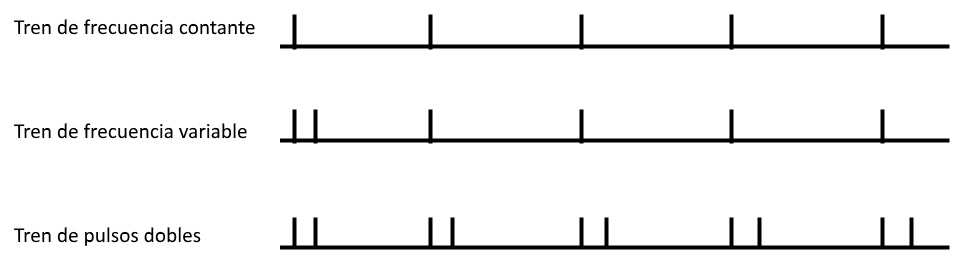
\includegraphics[scale=0.5]{tipos_repeticion}
  \caption{Tipos de trenes de pulsos según su periodo inter pulso. Cada línea vertical indica un pulso de corriente.}\label{fig:tipos_repeticion}
\end{figure}

Se muestra en la figura \ref{fig:tren_pulsos} un tren de pulsos bifásicos asmétricos y sus parámetros ya explicados.\\

\begin{figure}[!htb]
\centering
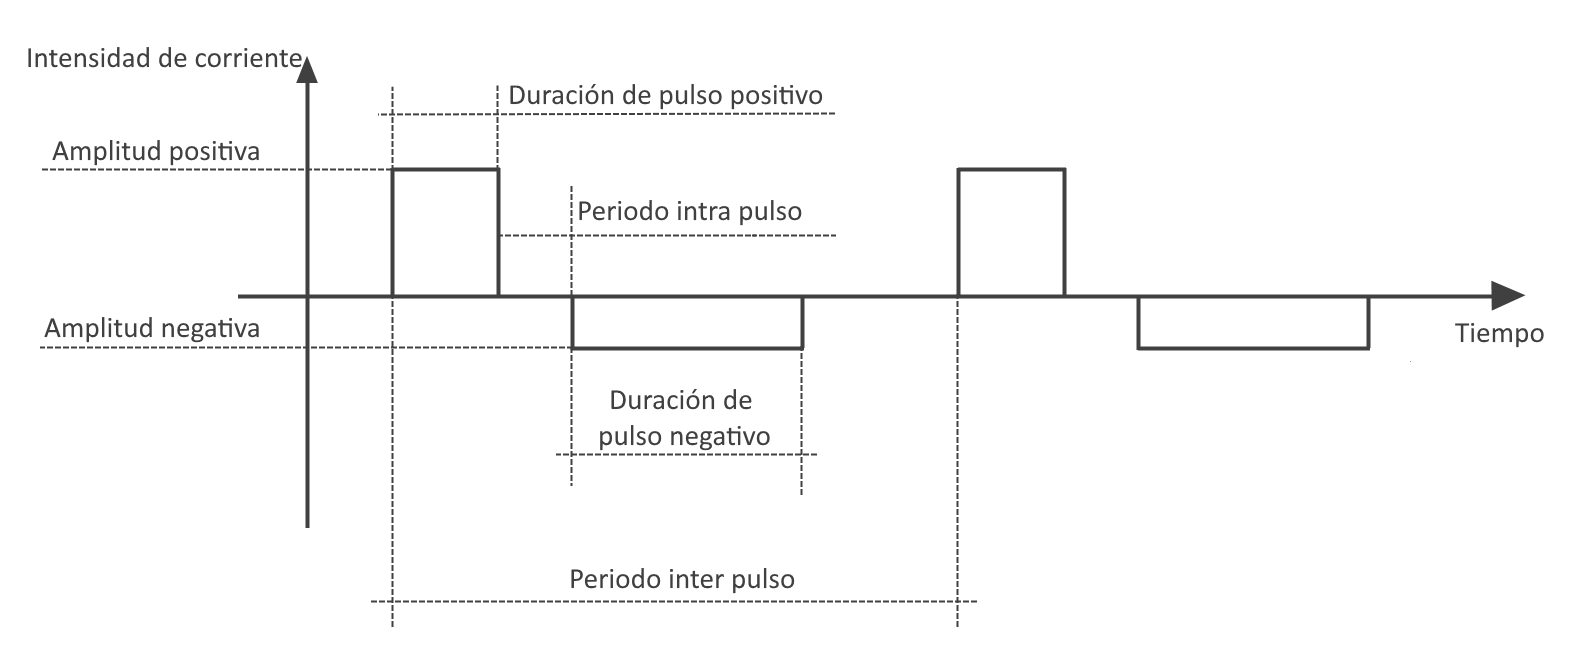
\includegraphics[scale=0.4]{tren_pulsos}
  \caption{Tren de pulsos bifásicos asimétricos.}\label{fig:tren_pulsos}
\end{figure}


El uso de la electroestimulación tiene beneficios como refuerzo de músculos, mejora de la circulación sanguínea, reducción de sensación de dolor y retraso de la atrofia muscular y de la espasticidad\cite{ventajas_FES}. Por otra parte, también existen desventajas como puede ser daño y fatiga muscular y alteraciones en la fuerza y tejidos y fibras musculares\cite{electroestimulacion}. Además, existen limitaciones en la aplicación de esta tecnología para neuro-rehabilitación y que son intrínsecas a la activación de músculos mediante estimulación eléctrica. En primer lugar, la respuesta al estímulo no es lineal y varía con el tiempo. Además, el músculo se va fatigando lo que altera su comportamiento el cual también varía según la resistencia a la fatiga y fuerza muscular. Por último, hay que considerar que hay un retardo considerable entre la generación del estímulo y  la respuesta por parte del músculo\cite{limitaciones_fes}.
\\
\\
Como ejemplo de aplicación de la electroestimulación se tiene el dispositivo comercial de Odstock\cite{estimulador_odstock} que permite corregir el pie caído\cite{pie_caido}. Dispone de un único canal, es decir, una salida por la que transmitir un tren de pulsos mediante el uso de electrodos superficiales sobre el nervio peroneo. Se muestra este dispositivo en la figura \ref{fig:estimulador_odstock}\\

\begin{figure}[!htb]
\centering
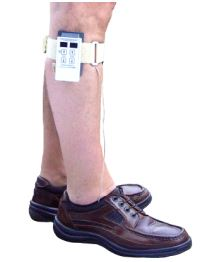
\includegraphics[scale=0.8]{estimulador_odstock}
  \caption{Electroestimulador de Odstock para el pie caído.}\label{fig:estimulador_odstock}
\end{figure}


\subsubsection{Prótesis híbridas}\label{protesis_hibridas}
Se han revisado las tecnologías de electroestimulación muscular y exoesqueletos robóticos para la asistencia en le neuro-rehabilitación de la marcha patológica. Ambas otorgan ventajas únicas pero al mismo tiempo implican ciertas limitaciones. Es por ello por lo que es posible combinar  FES y exoesqueletos robóticos, para potenciar sus ventajas y mitigar sus limitaciones durante la neuro-rehabilitación, la cual es mucho más eficaz en esta configuración de tecnologías que utilizando cualquiera de ellas de forma independiente\cite{protesis_hibridas}.
\\
\\
En primer lugar, se puede hablar de las neuroprótesis híbridas, las cuales combinan la tecnología FES para producir movimiento mediante contracciones musculares con un exoesqueleto pasivo o no motriz. De este modo, toda la actividad motriz proviene de la eslectroestimulación, es decir, de los músculos del paciente, mientras que el exoesqueleto se encarga de aportar estabilidad bloqueando articulaciones cuando sea necesario o asistiendo en determinados movimientos.
\\
\\
Partiendo de la configuración anterior, es posible el uso de la tecnología FES junto a un exoesqueleto motriz para abordar la mayor cantidad de casos en la neuro-rehabilitación de la marcha patológica. Una de las diferentes soluciones existentes implica un control cooperativo de los motores del exoesqueleto y la estimulación muscular. Esto consigue minimizar la contribución del torque ofrecido por el exoesqueleto y así maximizar la fuerza generada por los músculos mediante electroestimulación con parches superficiales\cite{FES_exoesqueleto_motriz}. Por un lado, el control del torque de los motores se consigue con una realimentación de la medida de ángulos de flexión de cadera y rodillas para seguir una trayectoria predefinida. Por otra parte, el control de la estimulación muscular se lleva a cabo mediante una estimación del momento de las articulaciones. Efectivamente, esta configuración ha sido probada en tres sujetos con diferentes niveles de lesión medular y todos ellos han mostrado un ciclo de marcha consistente y repetible con una actuación reducida por parte del exoesqueleto\cite{FES_exoesqueleto_motriz}.
\\
\\
Se considera entonces que existen dos principales tecnologías con el mejor potencial para una neuro-rehabilitación efectiva: FES y exoesqueletos motrices. Además, se ha demostrado que su combinación impulsa los beneficios y resultados más allá del uso individual de una de estas dos técnicas. Sin embargo, se puede dar un paso más y hacer uso de electrodos implantados para la electroestimulación funcional. A diferencia de los electrodos superficiales, un implante produce contracciones musculares más fuertes, consistentes y selectivas que cualquier otra técnica de electroestimulación, incluso para músculos con elevado grado de parálisis. De este modo, se da prioridad a los músculos del sujeto como fuente de movimiento potenciando así las ventajas que conlleva la estimulación eléctrica muscular ya discutidas previamente. Por tanto, el exoesqueleto motriz queda en un segundo plano para asistir al sujeto cuando lo necesite, por ejemplo, cuando sus músculos comiencen a fatigarse o en el caso de desviarse de la trayectoria adecuada. Esta configuración permite la utilización de exoesqueletos más ligeros debido a su papel secundario en la neuro-rehabilitación y de los cuales se puede incluso prescindir en determinadas actividades haciendo uso solamente de la electroestimulación. Se puede apreciar un ejemplo de este tipo de prótesis híbrida en la figura \ref{fig:protesis_hibrida}.\\

\begin{figure}[!htb]
\centering
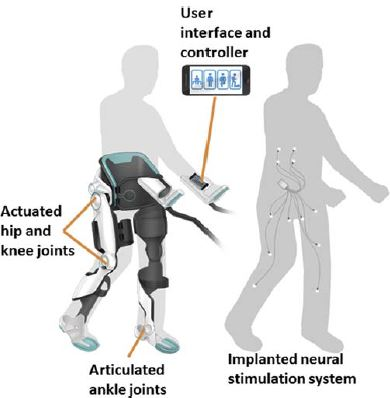
\includegraphics[scale=1.0]{protesis_hibrida}
  \caption{Modelo de prótesis híbrida que combina FES y un exoesqueleto motriz\cite{protesis_hibridas}.}\label{fig:protesis_hibrida}
\end{figure}

A pesar de los progresos realizados en las tecnologías para la neuro-rehabilitación, todavía existen limitaciones tales como la velocidad de la marcha y la comodidad y sencillez para usar diferentes tipos de prótesis. En cuanto al primer problema, se consideran 0.8$m/s$ y 500$m$ como velocidad y distancia promedio aceptables para la deambulación comunitaria\cite{requerimientos_ambulacion_1}\cite{requerimientos_ambulacion_2}, es decir, la realización de tareas básicas en el entorno donde reside el paciente como por ejemplo ir a comprar. Sin embargo, las tecnologías mencionadas no siempre consiguen que el paciente alcance dichos valores quedándose en 0.2-0.4$m/s$ usando solamente electroestimulación\cite{velocidad_FES} y 0.22-0.27$m/s$\cite{velocidad_exoesqueleto_1}\cite{velocidad_exoesqueleto_2} y hasta 170$m$\cite{distancia_exoesqueleto} valiéndose únicamente del exoesqueleto motriz. Pero estos valores dependen en gran medida de cada paciente ya que tanto la velocidad de marcha como la distancia máxima que puede realizar dependen notablemente de la fuerza y resistencia de la mitad superior del cuerpo. Esto se debe a que un exoesqueleto motriz requiere una fuerza considerable por parte de los brazos y el tronco para aportar estabilidad y asistir con la propulsión en la marcha. En cuanto al segundo problema, cualquier tipo de prótesis ya sea híbrida o solamente un exoesqueleto o electroestimulador, requiere ser calibrada antes de utilizarse, colocar los parches sobre la piel correctamente, tener las baterías cargadas en el caso correspondiente etc. Por tanto, es importante que estas preparaciones sean lo más rápidas y sencillas posible para facilitar la neuro-rehabilitación y evitar su abandono.


\subsubsection{Sensores}

Hasta ahora se ha hablado de actuadores como exoesqueletos robóticos y electroestimulación como tecnologías para la neuro-rehabilitación de la marcha patológica. Sin embargo, no se ha mencionado el control de mencionadas herramientas, el cual se va a discutir en este apartado. 
\\
\\
El control de un exoesqueleto, un dispositivo de electroestimulación o cualquier sistema puede realizarse en lazo abierto o en lazo cerrado. El primero de ellos implica el uso de estas herramientas de neuro-rehabilitación configuradas para una tarea determinada sin ningún tipo de información del ambiente, es decir, el paciente que interactúa con ellas. En cambio, si se dispone de información del estado del paciente y/o de la herramienta de neuro-rehabilitación durante la realización del ejercicio para detectar las fases de la marcha, existe mucho más control sobre el proceso así como resultados más satisfactorios y precisos. Para ello, se necesita sensar determinados parámetros de importancia para la correcta realización de los ejercicios de neuro-rehabilitación. Se muestran a continuación algunos de los sensores y medición de parámetros más comunes\cite{sensores}:

\begin{itemize}
\item[•] \textbf{Unidad de Medidas Inerciales:} Tienen gran capacidad de sensar los movimientos del cuerpo mediante acelerómetros y giróscopos cada vez más adaptables al ser humano debido a su reducción de tamaño y peso. En este sentido, se puede obtener información tridimensional midiendo aceleraciones, ángulos y velocidades angulares en los tres ejes espaciales. La principal ventaja de este sensor es que solamente necesita un punto de sujeción sobre el paciente o exoesqueleto.

\item[•] \textbf{Goniómetros:} Se utilizan para medir ángulos entre las dos partes de un miembro unidas por una articulación, por ejemplo, el ángulo entre la tibia y el fémur medido desde la rodilla. Existen goniómetros flexibles y en forma de potenciómetros aunque son muy sensibles debido a que están colocados en una articulación y necesitan dos puntos de sujeción.

\item[•] \textbf{Consumo de corriente en motores:} En el caso de los exoesqueletos, se puede medir el consumo de corriente de sus motores. Esto es útil ya que un motor de corriente continua al que se le restringe el movimiento responderá consumiendo más corriente para vencer esta resistencia. Por lo tanto, se pude tomar como indicativo de que el paciente está ejerciendo fuerza contra el exoesqueleto, es decir, se desvía de la trayectoria prevista. 

\item[•] \textbf{Sensor de fuerza resistivo:} Se utilizan principalmente para medir fuerza y distribución normal de presión en la pisada durante la fase del ciclo de marcha correspondiente. Sin embargo, no son indicados para medir fuerzas de corte o de cizalla. 

\item[•] \textbf{Electromiografía (EMG):} La electromiografía es un procedimiento mediante el cual se puede registrar la actividad eléctrica muscular denominada electromiograma. Esto permite determinar el estado de salud muscular así como el de las neuronas motoras que controlan los músculos esqueléticos\cite{EMG}. En el ámbito de la neuro-rehabilitación, se utiliza para obtener un mayor control sobre el estado de los músculos así como de su nivel de fatiga. Esto permite reforzar el aprendizaje del paciente mediante el ajuste de parámetros en el entrenamiento midiendo la intesidad con la que se activa cada músculo en todo momento\cite{EMG2}. La medición de esta actividad eléctrica se recoge en electrodos superficiales o transcutáneos (una fina aguja fina con el electrodo en forma de cable por dentro) Los primeros son más cómodos y no se descolocan con la actividad física pero arrojan mediciones más imprecisas. Los segundos ofrecen mayor calidad en las mediciones pero pueden ser dolorosos y perder efectividad ante movimientos bruscos, como pueden ser los del ciclo de marcha. Sin embargo, esta técnica no es fácilmente aplicable ya que puede resultar tedioso obtener mediciones correctas, especialmente en pacientes con sobrepeso u obesidad puesto que será más difícil llegar al músculo para medir su actividad.
\end{itemize}

%Una vez analizados algunos de los sensores utilizados en la electroestimulación y exoesqueletos, el tipo de control, objetivos y limitaciones del proceso de neuro-rehabilitación dependerá de cada aplicación así como del paciente. Consultando el estado del arte de los exoesqueletos para neuro-rehabilitación\cite{control_exoesqueleto}, destaca el control de impedancias o admitancias del exoesqueleto hacia el paciente, es decir, cómo de permisivo o resistivo es este dispositivo ante determinados movimientos del paciente. Por otra parte, se puede controlar la actuación de un electroestimulador en función de la actividad muscular medida mediante electromiografía. De este modo, se modula la intensidad de le electroestimulación para minimizar el error entre la trayectoria efectuada por el paciente y la trayectoria objetivo de forma iterativa\cite{control_FES}. 

%Para concluir, y sin entrar en mayor detalle técnico, estos tipos de controles se pueden implementar mediante controladores PID o métodos de aprendizaje iterativos, entre otros, ya que el ciclo de marcha es un proceso altamente repetitivo\cite{tesis_antonio}. Es importante una elección adecuada de los tipos de control y su implementación teniendo en cuenta el tipo de lesión que se quiere rehabilitar dentro de las explicadas en el apartado \ref{clasificacion_lesiones}. Además, no hay que olvidar que el ciclo de marcha es un proceso complejo y difícil de replicar.


\subsubsection{Revisión del estado del arte de neuroprótesis para el pie caído}
Para profundizar en uno de los tópicos dominantes en el presente trabajo, la neuro-rehabilitación mediante neuroprótesis, se ha estudiado una revisión del estado del arte de neuroprótesis para el pie caído\cite{estado_arte_FES}. Esta revisión plantea en primer lugar un esquema de la arquitectura de una neuroprótesis genérica para pie caído y que se aprecia en la figura \ref{fig:esquema_FES}.\\
 
\begin{figure}[!htb]
\centering
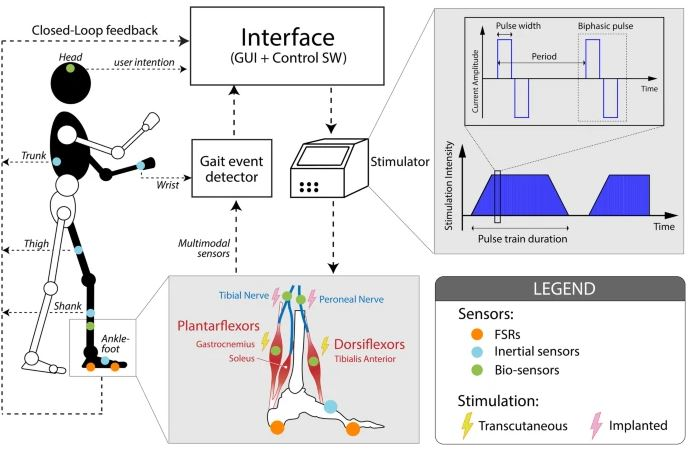
\includegraphics[scale=0.8]{esquema_FES}
  \caption{Arquitectura de una neuroprótesis para pie caído en lazo cerrado. Se utilizan sensores para detectar la fase del ciclo de marcha y estimular eléctricamente en consecencia\cite{estado_arte_FES}.}\label{fig:esquema_FES}
\end{figure}

Prosiguiendo con el análisis de la mencionada revisión, ésta lleva a cabo una clasificación de neuroprótesis para pie caído según diferentes parámetros. Antes de entrar en detalle en dicha clasificación, se ha de mencionar que esta revisión recoge publicaciones que tratan avances tecnológicos en cuanto a diseño y arquitectura de control, así como resultados clínicos provenientes de este tipo de prótesis. Para ello, se tienen en cuenta publicaciones en las bases de datos de PubMed, PEDro, SCOPUS, Academic Google, MEDLINE, EMBASE, ResearchGate, WoS, and SciELO. Además, se tienen como criterios de búsqueda publicaciones entre los años 2000 y 2018, estudios que presenten neuroprótesis para pie caído, estudios presentados en revistas o conferencias, tesis o catálogos y se excluyen todos los estudios que traten sobre prótesis híbridas.
\\
\\
Siguiendo con la clasificación mencionada previamente, esta revisión del estado del arte crea dos grupos de neuroprótesis según su tipo de control: lazo abierto y lazo cerrado. Además, independientemente del tipo de control se crea otra clasificación según el tipo de sensores embarcados en la neuroprótesis: resistivos, inerciales y biosensores. Además, como categorías secundarias, se diferencia entre neuroprótesis para investigación o comercial, transcutánea o implantada y se especifica su número de canales así como el tipo de movimiento en el que asiste al paciente. De este modo, se recoge en la figura \ref{fig:clasificacion_estado_arte_FES} todas las neuroprótesis encontradas acorde los criterios de búsqueda y clasificadas según los parámetros mencionados.\\

\begin{figure}[!htb]
\centering
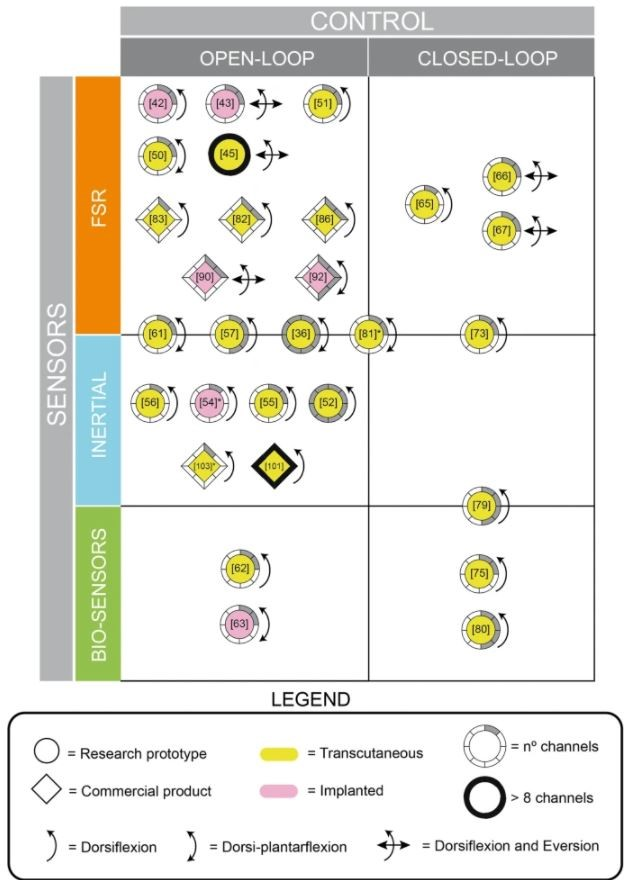
\includegraphics[scale=0.8]{clasificacion_estado_arte_FES}
  \caption{Clasificación de neuroprótesis para pie caído\cite{estado_arte_FES}.}\label{fig:clasificacion_estado_arte_FES}
\end{figure}

La revisión estudia todas las neuroprótesis expuestas en la figura anterior las cuales no se van a exponer en el presente trabajo por cuestiones de brevedad. Sin embargo, es importante destacar las conclusiones de dicha revisión ya que supone una puesta en común de fortalezas y debilidades de este tipo de prótesis además de plantear directrices y vías de mejora. 
\\
\\
En primer lugar, es importante destacar que se han hecho progresos importantes durante las últimas dos décadas en cuanto a la arquitectura de las neuroprótesis y las estrategias para obtener mejores resultados en la neuro-rehabilitación. De hecho, muchas de ellas tienen uso comercial, es decir, fuera de laboratorios y centros especializados para dotar de mayor libertad al paciente que las necesite. Sin embargo, todavía existen limitaciones en el uso de este tipo de prótesis siendo la principal de ellas la fatiga muscular provocada por la electroestimulación de forma continuada y la cual debe gestionarse. Además, se ha observado una falta en el desarrollo de sistemas bilaterales, es decir, para asistir ambas extremidades. 
\\
\\
Como vías de mejora, es importante desarrollar la estrategia de assist-as-need (AAN), mencionada con anterioridad en este capítulo, además del control en lazo cerrado el cual permite una neuro-reahabilitación dinámica e individualizada. Otra rama de desarrollo implica el uso de electrodos transcutáneos con un ajuste automático, lo cual permite utilizar la neuroprótesis fuera de clínicas y centros especializados. Esto permite una mayor adaptación segura del ciclo de marcha en diferentes entornos de la vida diaria como pueden ser escaleras o superficies inclinadas. En cuanto a las técnicas de electroestimulación, la combinación de pulsos de frecuencia constante (CFT) y frecuencia variable (VFT) es prometedora en cuanto a la reducción de fatiga muscular. Por último, se considera de gran importancia el desarrollo de estudios de largo alcance para la medición de la actividad muscular durante la marcha para una mejor comprensión y cuantificación de los mecanismos implicados en el ciclo de marcha y neuro-rehabilitación de cada paciente.


\section{Objetivos del trabajo}
Tal y como se ha mencionado en el presente capítulo, el autor del trabajo lo ha realizado en el grupo de neuro-rehabilitación del Instituto Cajal. Dicho grupo desarrolla un proyecto que tiene lugar en un ámbito de investigación de la neuro-rehabilitación de la marcha patológica en continuo desarrollo. Se parte de la idea del uso de sistemas neuro-mecánicos (electroestimulación en conjunto a sistemas mecánicos como un exoesqueleto) para unificar sus ventajas y minimizar sus limitaciones. Esta combinación resulta más ventajosa que utilizar cualquiera de sus componentes por separado, tal y como se vio en el apartado \ref{protesis_hibridas}. De hecho, se puede incluso conseguir que pacientes con paraplejia sean capaces de levantarse o sentarse, caminar y subir o bajar escaleras.
\\
\\
Teniendo en cuenta el marco en el que se sitúa el presente Trabajo Fin de Máster, se procede a explicar cómo encaja en el equipo de neuro-rehabilitación y su objetivo final. El proyecto que desarrolla el equipo se centra en la neuro-rehabilitación de la marcha patológica debida a daños en el sistema nervioso central causados por lesiones medulares e ictus\cite{tesis_antonio}. Para ello, está desarrollando una prótesis híbrida cuyos componentes son los siguientes:

\begin{itemize}
\item[•] Un exoesqueleto robótico capaz de generar movimiento
\item[•] Neuroprótesis modular para el control neuromuscular en red mediante electroestimulación funcional o FES
\item[•] Conjunto de sensores 
\end{itemize}

Además, se está desarrollando un subproyecto del anterior con los siguientes objetivos:
\begin{itemize}
\item[•] Diseño y desarrollo de la neuroprótesis modular
\item[•] Integración de la neuroprótesis con el exoesqueleto 
\item[•] Validación de la neuroprótesis para su aplicación en control híbrido con el exoesqueleto
\end{itemize}

La neuroprótesis, tal y como se ha mencionado, es modular lo que significa que se puede hacer uso de hasta cuatro dispositivos de electroestimulación independientes. Estos se explicarán en mayor detalle en el siguiente capítulo así como el resto de componentes de la neuroprótesis. Sin embargo, cabe destacar en este punto que se pretende efectuar un control y configuración de la prótesis híbrida desde un ordenador de forma inalámbrica, para mayor comodidad y flexibilidad en la neuro-rehabilitación de la marcha patológica. 
\\
\\
\textbf{El autor del presente Trabajo Fin de Máster participa tanto en el proyecto principal como en el subproyecto y colabora en todos los objetivos expuestos. Por tanto, las contribuciones al proyecto y objetivos del trabajo son:}

\begin{itemize}
\item[\textbf{1)}] \textbf{Selección y programación de un microcontrolador para el control centralizado de la prótesis híbrida con las siguientes funciones:}
\begin{itemize}
\item[a)] Recibir y procesar las mediciones arrojadas por el exoesqueleto y el conjunto de sensores utilizado.

\item[b)] Controlar de forma simultánea y en tiempo real hasta cuatro dispositivos de electroesimulación en función de la información recibida por los sensores. Esto implica modificar el comportamiento de los dispositivos de estimulación durante la realización del ejercicio de rehabilitación.

\item[c)] Controlar en tiempo real el exoesqueleto en función del estado de los electroestimuladores y las mediciones de los sensores.


\end{itemize}
\item[\textbf{2)}] \textbf{Desarrollo de una interfaz gráfica de usuario para para:}
\begin{itemize}
\item[a)] Establecer una configuración inicial de la prótesis para la tarea de rehabilitación correspondiente así como cargar y guardar perfiles de configuración. Esto se lleva a cabo mediante una comunicación directa entre la interfaz y el microcontrolador expuesto en el punto 1).

\item[b)] Visualizar en tiempo real las mediciones del conjunto de sensores utilizado.

\item[c)] Controlar el ejercicio de rehabilitación iniciando o deteniendo la transmisión de datos de los sensores y el exoesqueleto así como la estimulación eléctrica.
\end{itemize}


\item[\textbf{3)}] \textbf{Revisión y mejora del hardware de los módulos de la neuroprótesis:}
\begin{itemize}
\item[a)] Revisión y mejora de las tarjetas de circuito impreso correspondientes a las etapas de control y potencia.
\end{itemize}

\item[\textbf{4)}] \textbf{Revisión y mejora del software de los módulos de la neuroprótesis:}
\begin{itemize}
\item[a)] Optimización de la comunicación con el dispositivo.
\end{itemize}
\end{itemize}

Una vez expuestos los objetivos del presente Trabajo Fin de Máster, se muestra en la figura \ref{fig:esquema_protesis_objetivos} un esquema generalizado de la prótesis híbrida en cuyo desarrollo participa el autor del trabajo y que supone el objetivo global del mismo. Se aprecia cómo el microcontrolador actúa de nodo central entre el exoesqueleto, electroestimuladores y sensores así cómo éste es accesible con un ordenador desde la interfaz gráfica de usuario mencionada previamente. No se pretende en este punto explicar en detalle el esquema ya que deben tratarse características tales como los protocolos de comunicación y propiedades del microcontrolador y resto de componentes de la prótesis. Dichos detalles se verán en su correspondiente capítulo.\\

\begin{figure}[!htb]
\centering
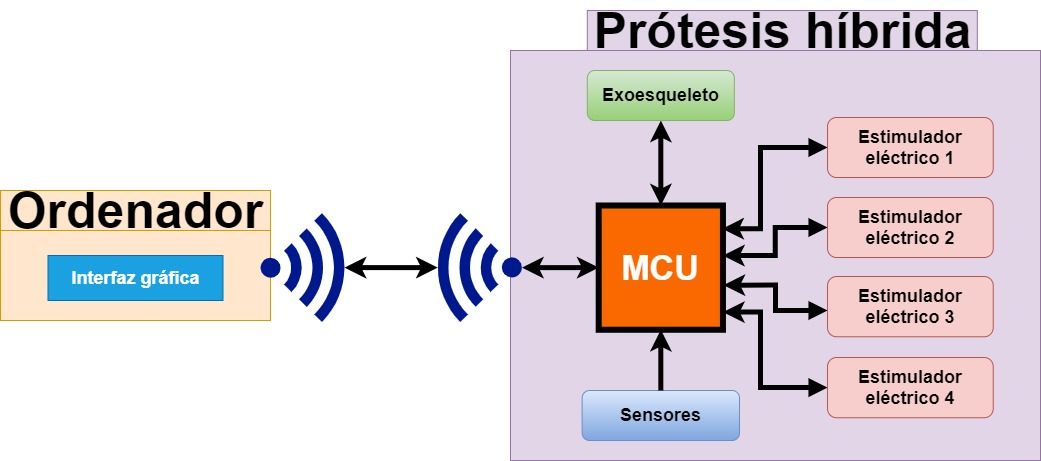
\includegraphics[scale=0.4]{esquema_protesis_objetivos}
  \caption{Esquema simplificado de la prótesis híbrida. Las flechas indican la comunicación entre los elementos unidos, bidireccional o unidireccional, sin especificar el protocolo.}\label{fig:esquema_protesis_objetivos}
\end{figure}


\chapter{Estudio de los componentes de la prótesis híbrida}\label{capitulo_2}
En el presente capítulo se va a explicar en mayor detalle cada uno de los componentes de la prótesis híbrida planteada en los objetivos del Trabajo Fin de Máster del capítulo introductorio.
\\
\\
Se pretende conocer en mayor profundidad cada componente y sus características en el estado que se encuentran al comienzo del presente trabajo, es decir, sin ningún tipo de modificación efectuada por el autor del mismo.
\\
\\
Terminada esta revisión y tras efectuar los cambios necesarios sobre cada componente de la prótesis a lo largo de los siguientes capítulos, se mostrará el montaje completo de la prótesis híbrida que se pretende construir.

\section{Electroestimulador muscular}
El electroestimulador utilizado en la prótesis híbrida ha sido desarrollado con anterioridad en el propio grupo de neurorrehabilitación del Insituto Cajal. Aparece en la figura \ref{fig:terefes} y se denomina mini TEREFES.\\

\begin{figure}[!htb]
\centering
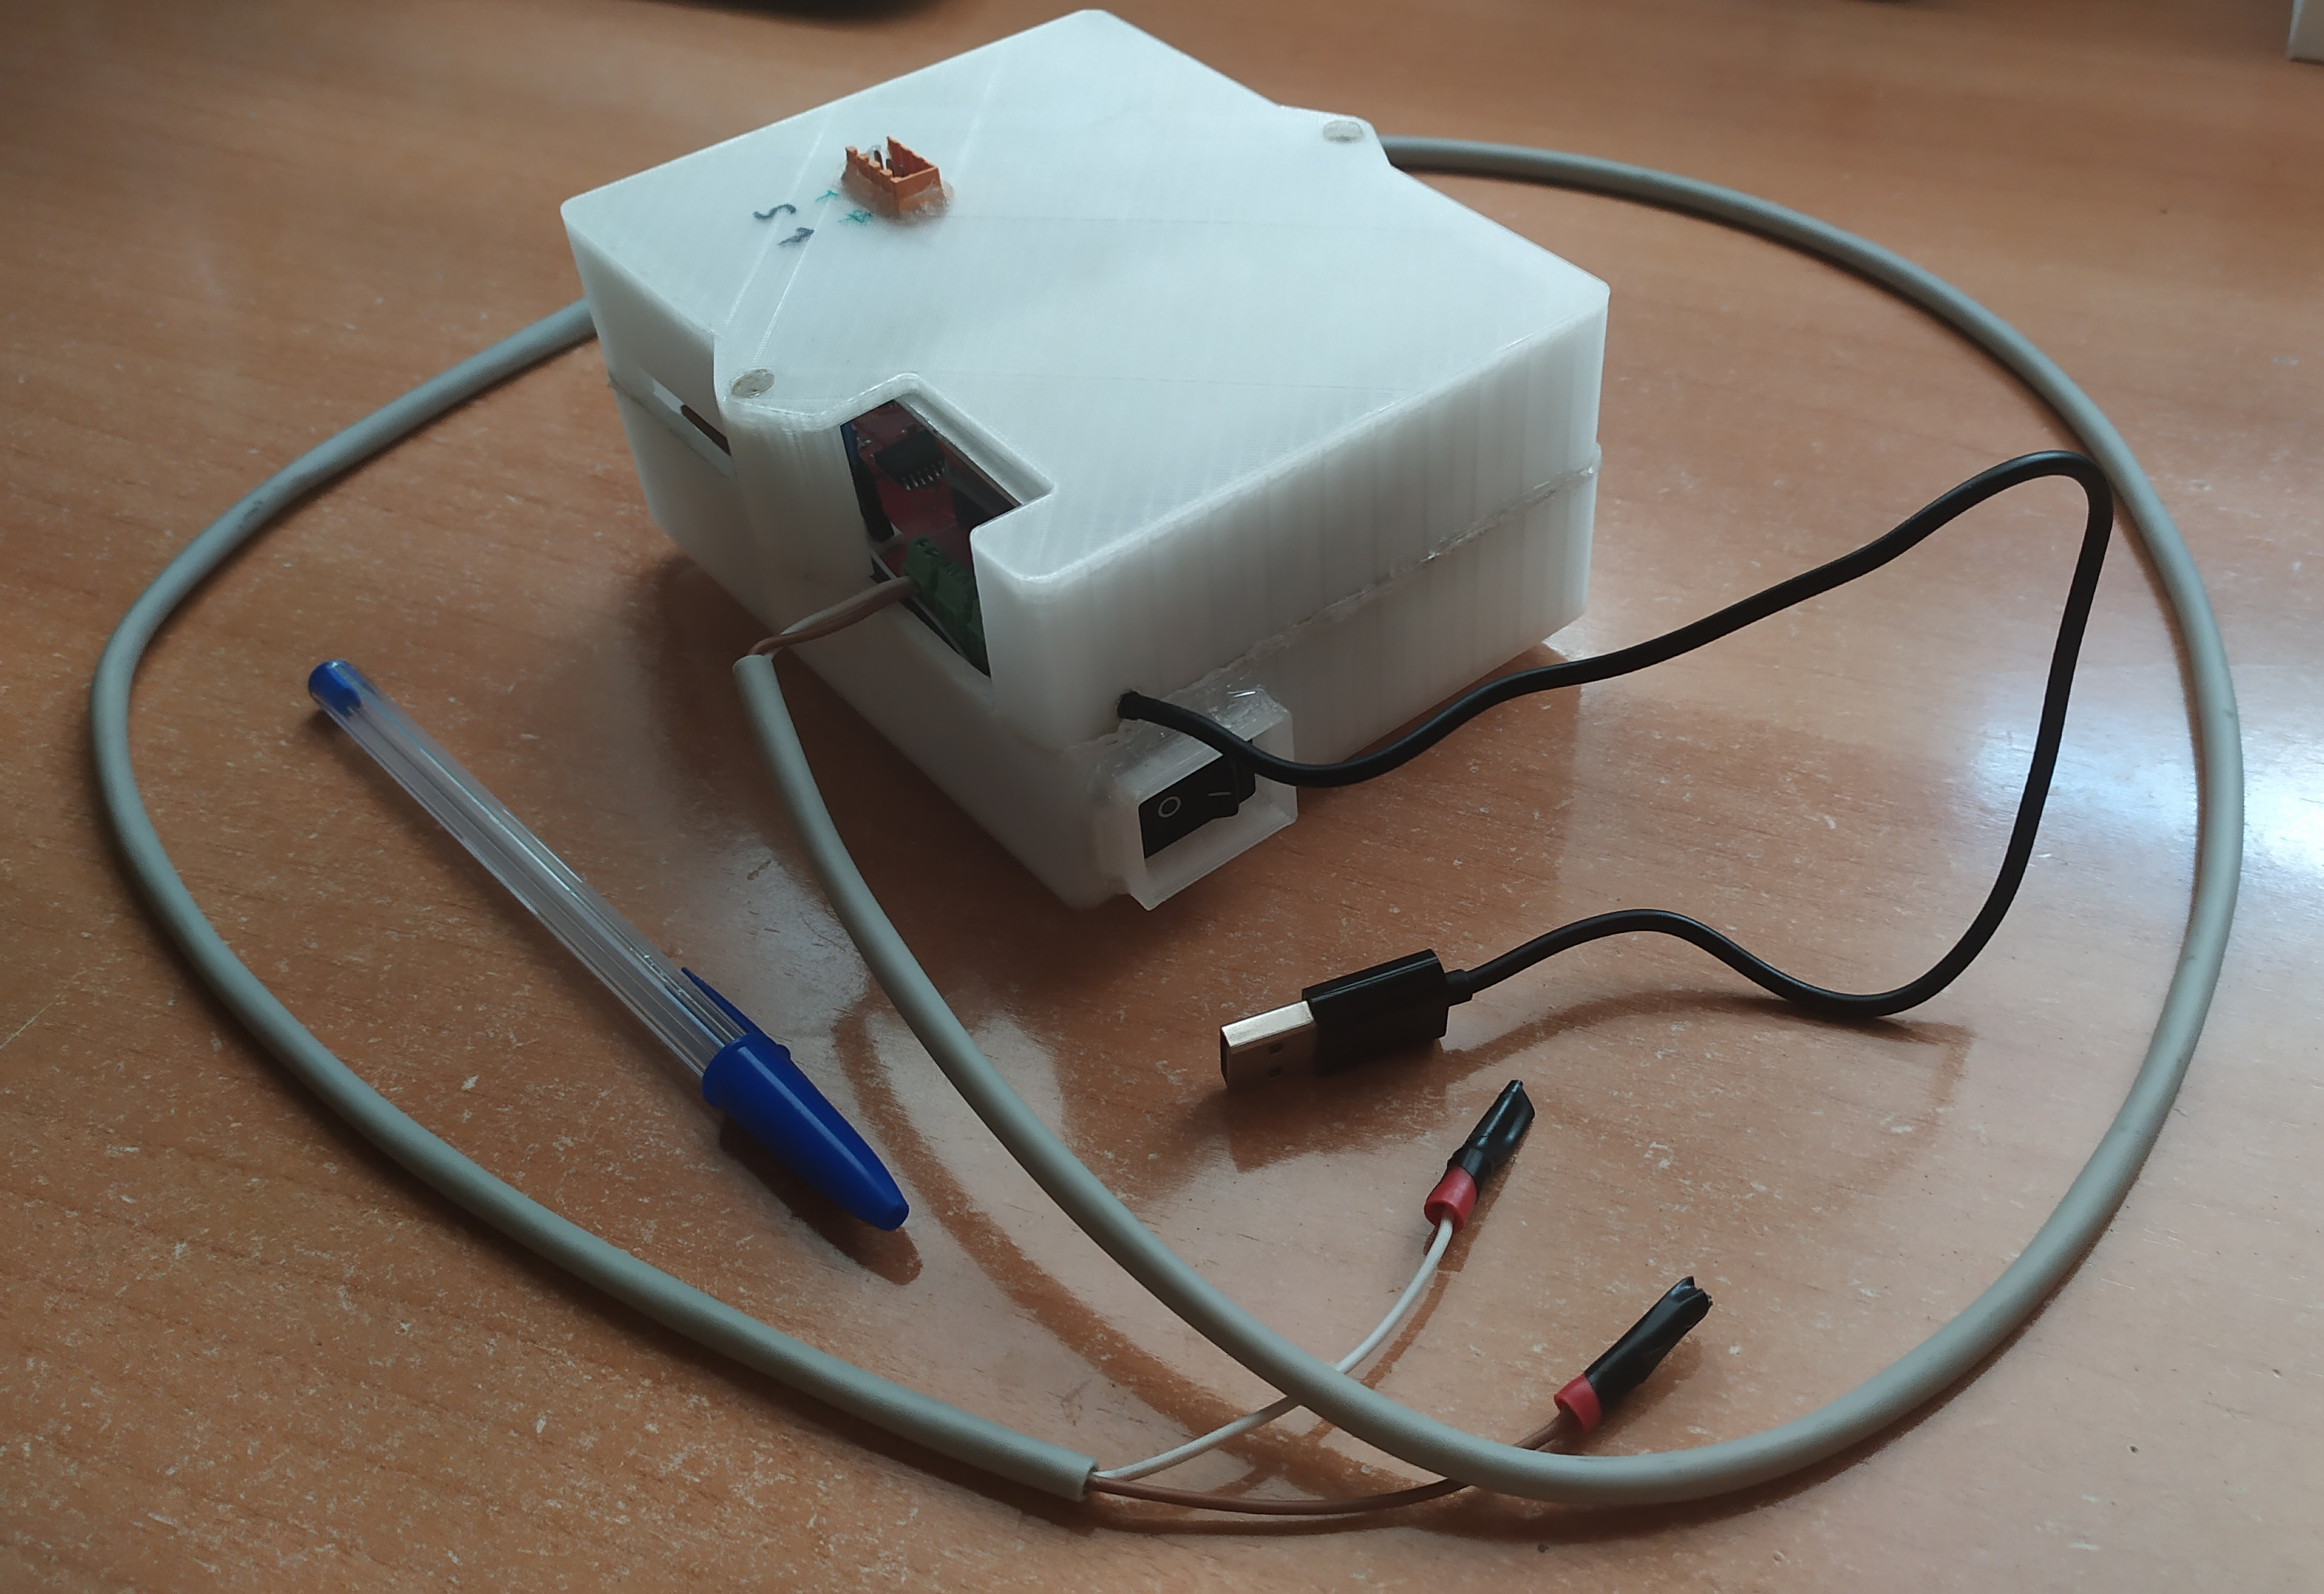
\includegraphics[scale=0.1]{terefes}
  \caption{Electroestimulador de 4 canales mini TEREFES. El cable negro USB tipo A permite la conexión a una fuente de 5V. El cable gris es la salida de uno de los canales con los extremos a los que iría el parche, sin conectar.}\label{fig:terefes}
\end{figure}

Este dispositivo dispone de 4 canales o salidas siendo cada una de ellas capaz de estimular un músculo o grupo de músculos. Esto lo hace mediante un par de electrodos conectados cada uno al estimulador con su respectivo cable. Se aprecian dichas salidas en la figura \ref{fig:canales}. Además, cada canal tiene su propia configuración de tren de pulsos de corriente, tal y como se ha explicado con anterioridad en los principios del funcionamiento de la electroestimulación. Se explicaron también una serie de parámetros de configuración del tren de pulsos de corriente y los cuales, para el caso del mini TEREFES, quedan recogidos en la tabla \ref{tabla:detalles_terefes}.\\


\begin{figure}[!htb]
\centering
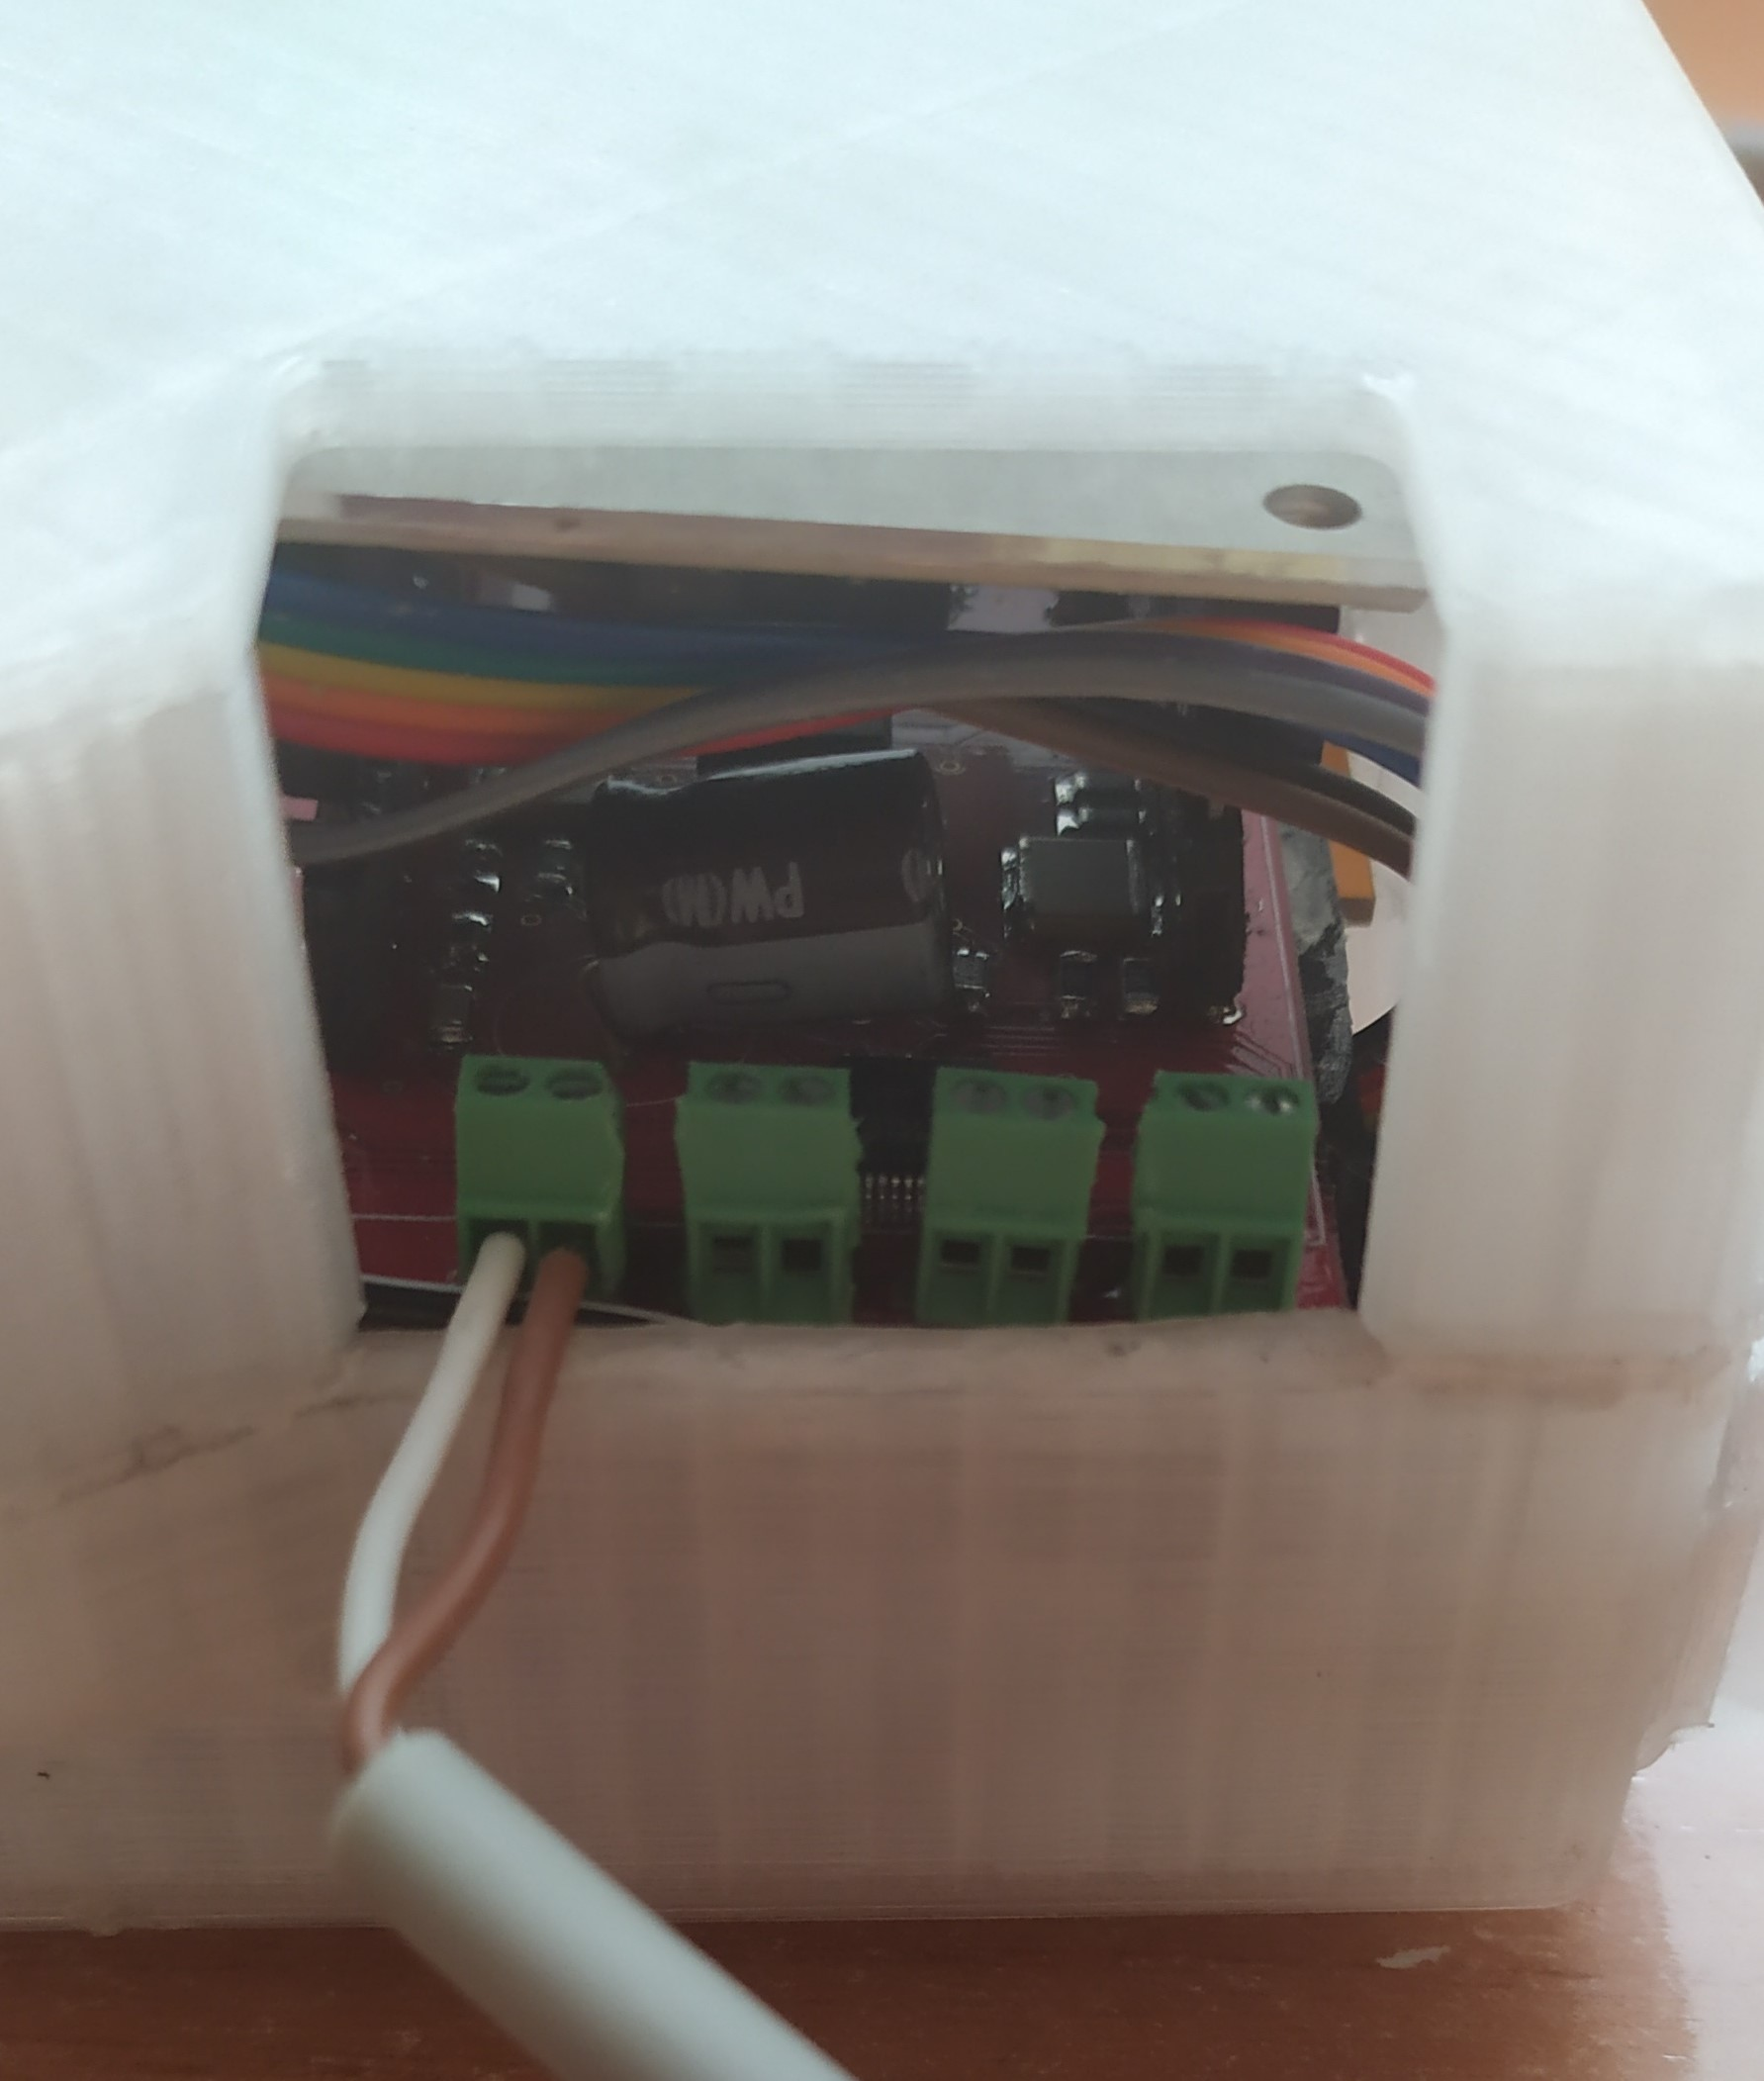
\includegraphics[scale=0.1]{canales}
  \caption{Conectores correspondientes a los 4 canales del estimulador.}\label{fig:canales}
\end{figure}

\begin{table}
\centering
\begin{tabular}{| p{30mm} | p{90 mm} |}
\hline
Corriente & De 0 a 90$mA$ en incrementos de 782.67$\mu A$ \\ \hline
Ancho de pulso & De 0 a 5000$\mu s$ en incrementos de 2.4$\mu s$\\ \hline
Frecuencia & Máximo de 100$Hz$ \\ \hline
Forma de pulso & Bifásico rectangular con tiempo interpulso de 100$\mu s$\\ \hline
Canales & Hasta 32 canales (dos módulos de 16 canales) de los que solamente se utilizan un máximo de 4\\ \hline
\end{tabular}\caption{Características del TEREFES.}\label{tabla:detalles_terefes}
\end{table}

El estimulador no dispone de batería interna por lo que es necesario alimentarlo a 5V mediante un cable USB tipo A. Para mayor portabilidad, y debido al voltaje y amperaje que maneja este dispositivo, cada estimulador dispone de una batería portátil de polímero de litio de $10000mAh$ y $5V$ a un máximo de $2.1A$ de descarga. Esta batería es similar a las utilizadas comúnmente para cargar teléfonos móviles y otros dispositivos de características parecidas.

\subsection{Hardware}
El hardware del electroestimulador tiene tres componentes principales:

\begin{itemize}
\item[•] Etapa de control
\item[•] Etapa de potencia
\item[•] Módulo de comunicación
\end{itemize}

\subsubsection{Etapa de control}
La etapa de control se encarga de la generación de la configuración de los trenes de pulsos de corriente para una correcta electroestimulación, aislamiento digital de estas señales y amplificación de las mismas. Sus principales componentes, en orden, desde la generación de la señal hasta su salida a los parches que se colocan en el paciente son:

\begin{itemize}
\item[1)] Un Microcontrolador Atmel de 8 bits y arquitectura AVR-RISC ATmega128L que genera las señales de configuración del tren de pulsos de corriente, entre otras funciones de control.
\item[2)] Cinco aisladores digitales alimentados por un regulador de tensión de 15 a 5 voltios y conectados a las señales generadas por el microcontrolador.
\item[3)] Un convertidor digital/analógico (DAC) de 8 bits junto a una referencia de tensión de 10V.
\item[4)] Primera etapa de amplificación de la salida del DAC con un amplificador operacional.
\item[5)] Segunda etapa de amplificación mediante un amplificador operacional de potencia con el cual se implementa una fuente de corriente tipo Howland mostrada en la figura \ref{fig:howland}. Se eligió utilizar este tipo de fuente de corriente por su linealidad en la ganancia de corriente, así como una reducida disminución de la corriente de salida ante impedancias elevadas en la carga\cite{FES}.\\

\begin{figure}[!htb]
\centering
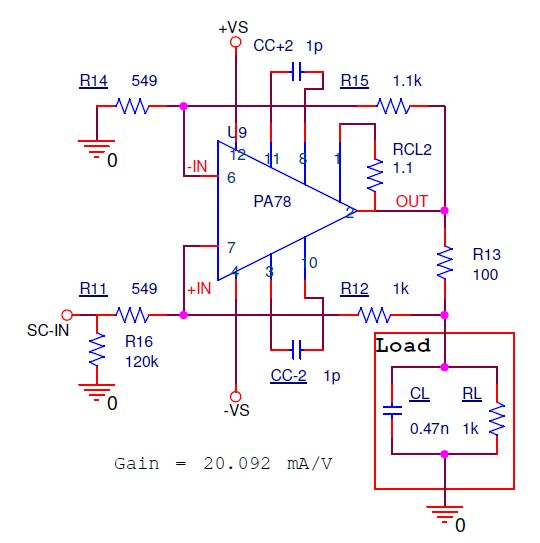
\includegraphics[scale=0.7]{howland}
  \caption{Fuente de corriente tipo Howland utilizada en el mini TEREFS\cite{FES}.}\label{fig:howland}
\end{figure}

\item[6)] Un switch analógico para controlar hasta cuatro canales o salidas, es decir, cuatro trenes de pulsos diferentes.
\end{itemize}

Se muestra en el Anexo I tanto el esquemático de esta etapa como la disposición de los componentes descritos en la tarjeta de circuito impreso.


\subsubsection{Etapa de potencia}\label{etapa_potencia}
La etapa de potencia se ha reciclado del TEREFES, estimulador del que procede el mini TEREFES. Esta se puede apreciar en el esquemático de la figura \ref{fig:fuente_terefes} y la cual está compuesta por dos fuentes de $\pm15VDC$ dos fuentes de $15VDC$ y una fuente de $5VDC$ que proporcionan dichos niveles de tensión a la etapa de control. Sin embargo, el mini TEREFES es un modelo más compacto y utiliza esta misma etapa de potencia pero prescindiendo de una de las fuentes de $15VDC$ y una de $\pm15VDC$ tal y como muestra el esquemático de la figura \ref{fig:fuente_mini_terefes}.\\

\begin{figure}[!htb]
\minipage{0.45\textwidth}
  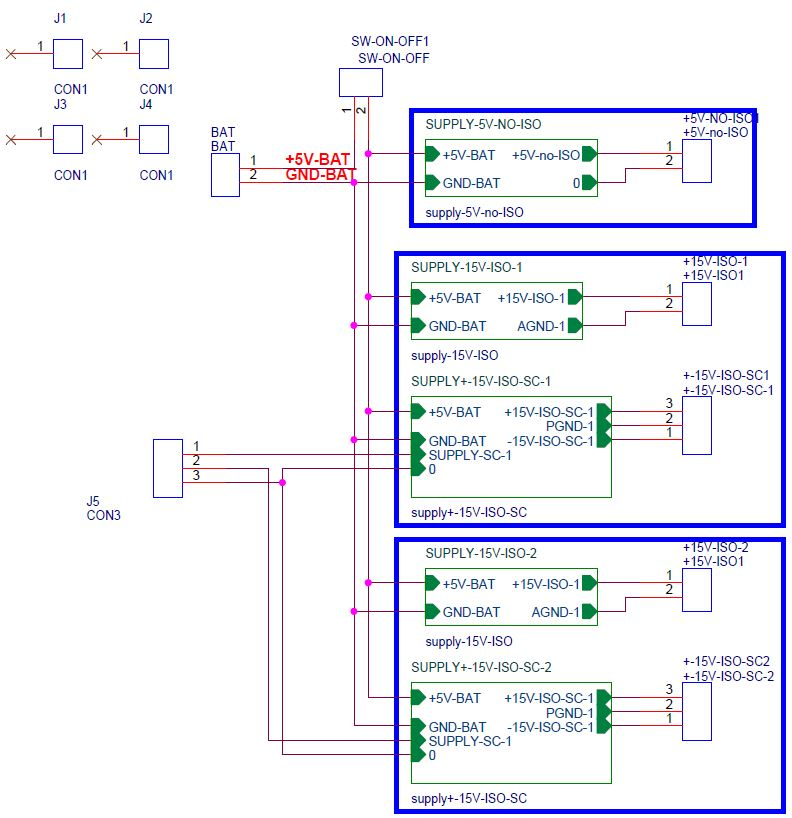
\includegraphics[width=\linewidth]{fuente_terefes}
  \caption{Esquemático de la etapa de potencia del TEREFES con alimentación a $5VDC$ de la batería (BAT), una fuente de $5VDC$ en cuadro el azul superior y dos fuentes de $15VDC$ y $\pm15VDC$, cada una de ellas en lod dos cuadros azules inferiores}\label{fig:fuente_terefes}
\endminipage\hfill
\minipage{0.45\textwidth}
  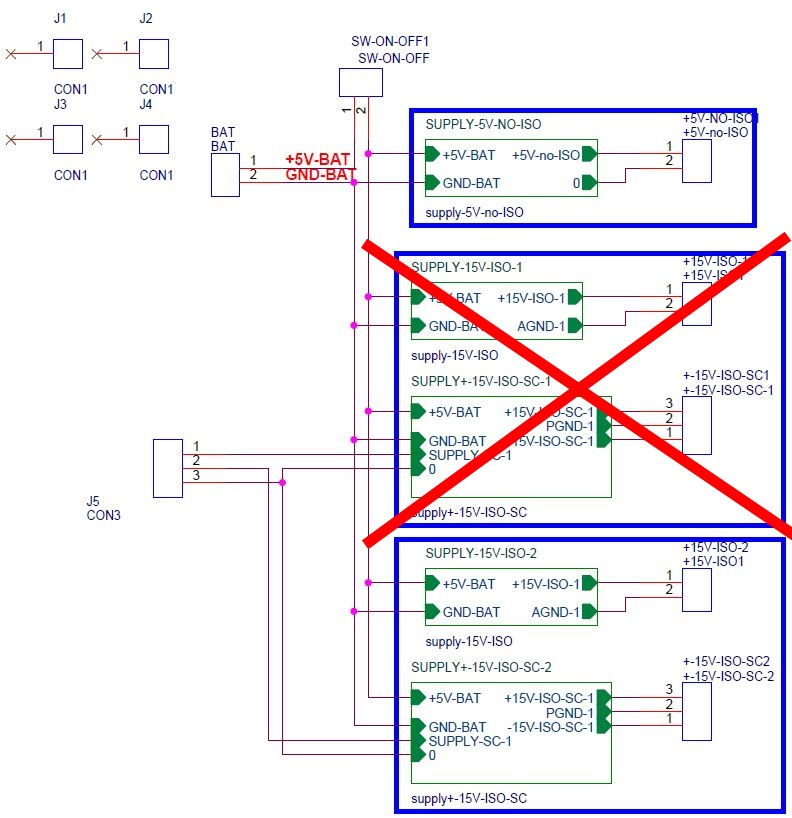
\includegraphics[width=\linewidth]{fuente_mini_terefes}
  \caption{Esquemático de la etapa de potencia del mini TEREFES con una fuente de $5VDC$ y otra de $15VDC$ y $\pm15VDC$}\label{fig:fuente_mini_terefes}
\endminipage\hfill
\end{figure}

La tarjeta de circuito impreso de la etapa de potencia recibe en su entrada $5VDC$ mediante el cable USB tipo A, tal y como se mencionó con anterioridad. Esta tensión alimenta a las fuentes de $5VDC$, $\pm15VDC$ y $15VDC$ las cuales están implementadas con los siguientes convertidores DC/DC:

\begin{itemize}
\item[•] Convertidor DC/DC de $5VDC$ a $5VDC$ a una corriente máxima de $400mA$.

\item[•] Convertidor DC/DC de $5VDC$ a $15VDC$ a una corriente máxima de $200mA$.

\item[•] Convertidor DC/DC de $5VDC$ a $\pm15VDC$ a una corriente máxima de $400mA$.
\end{itemize}

La etapa de potencia proporciona a la de control la alimentación a $5VDC$, $15VDC$ y $\pm15VDC$ utilizando los convertidores expuestos previamente. 

\subsubsection{Comunicación}
Existen dos formas de establecer comunicación con la etapa de control desde un dispositivo externo como puede ser un ordenador:

\begin{itemize}
\item[•] \textbf{Conexión In System Programming o ISP:} esta se usa para programar el microcontrolador mediante el conector ISP apreciable en el esquemático de la etapa de control en el Anexo I. Dado que el estimulador mini TEREFES utiliza un microcontrolador ATmega128L, que tiene arquitectura AVR-RISC, se hace uso del programador AVRISP mkII\cite{programador} para grabar el firmware. Dicho programador se puede ver en la figura \ref{fig:programador_micro}.

\item[•] \textbf{Interrupciones USART AVR:} se utilizan interrupciones para que el microcontrolador sea capaz de recibir y transmitir parámetros de configuración de la electroestimulación y otros datos. Para ello, se acopla al conector JP5 de la etapa de control el módulo Bluetooth Sparkfun Smirf Silver de la figura \ref{fig:modulo_bluetooth}. En dicho conector se tienen 4 pines: alimentación a 5V, pin de transmisión TX, pin de recepción RX y masa. De este modo, se establece conexión mediante un puerto serie virtual vía Bluetooth entre un ordenador y el módulo mencionado. Una vez establecida la conexión, el módulo Bluetooth sirve de intermediario entre el ordenador y el microcontrolador del estimulador para la transmisión de información. Se expondrán en mayor detalle todas las posibilidades de configuración en el apartado \ref{firmware}


%Otra forma de producir las interrupciones mencionadas y establecer comunicación entre un ordenador y el mini TEREFES es conectar mediante un cable un puerto USB del ordenador a los pines en los que se aloja el módulo Bluetooth. Sin embargo, es necesario utilizar un convertidor USB-USART, elemento no necesario si se utiliza el módulo Bluetooth pues éste ya hace esta conversión. Aún así, la velocidad de transmisión de datos siempre será superior en una conexión cableada frente a una inalámbrica. Se explorará esta opción en el capítulo correspondiente al estudio y mejora de la velocidad de transmisión de datos entre el microcontrolador y un dispositivo externo.

\end{itemize}

\begin{figure}[!htb]
\centering
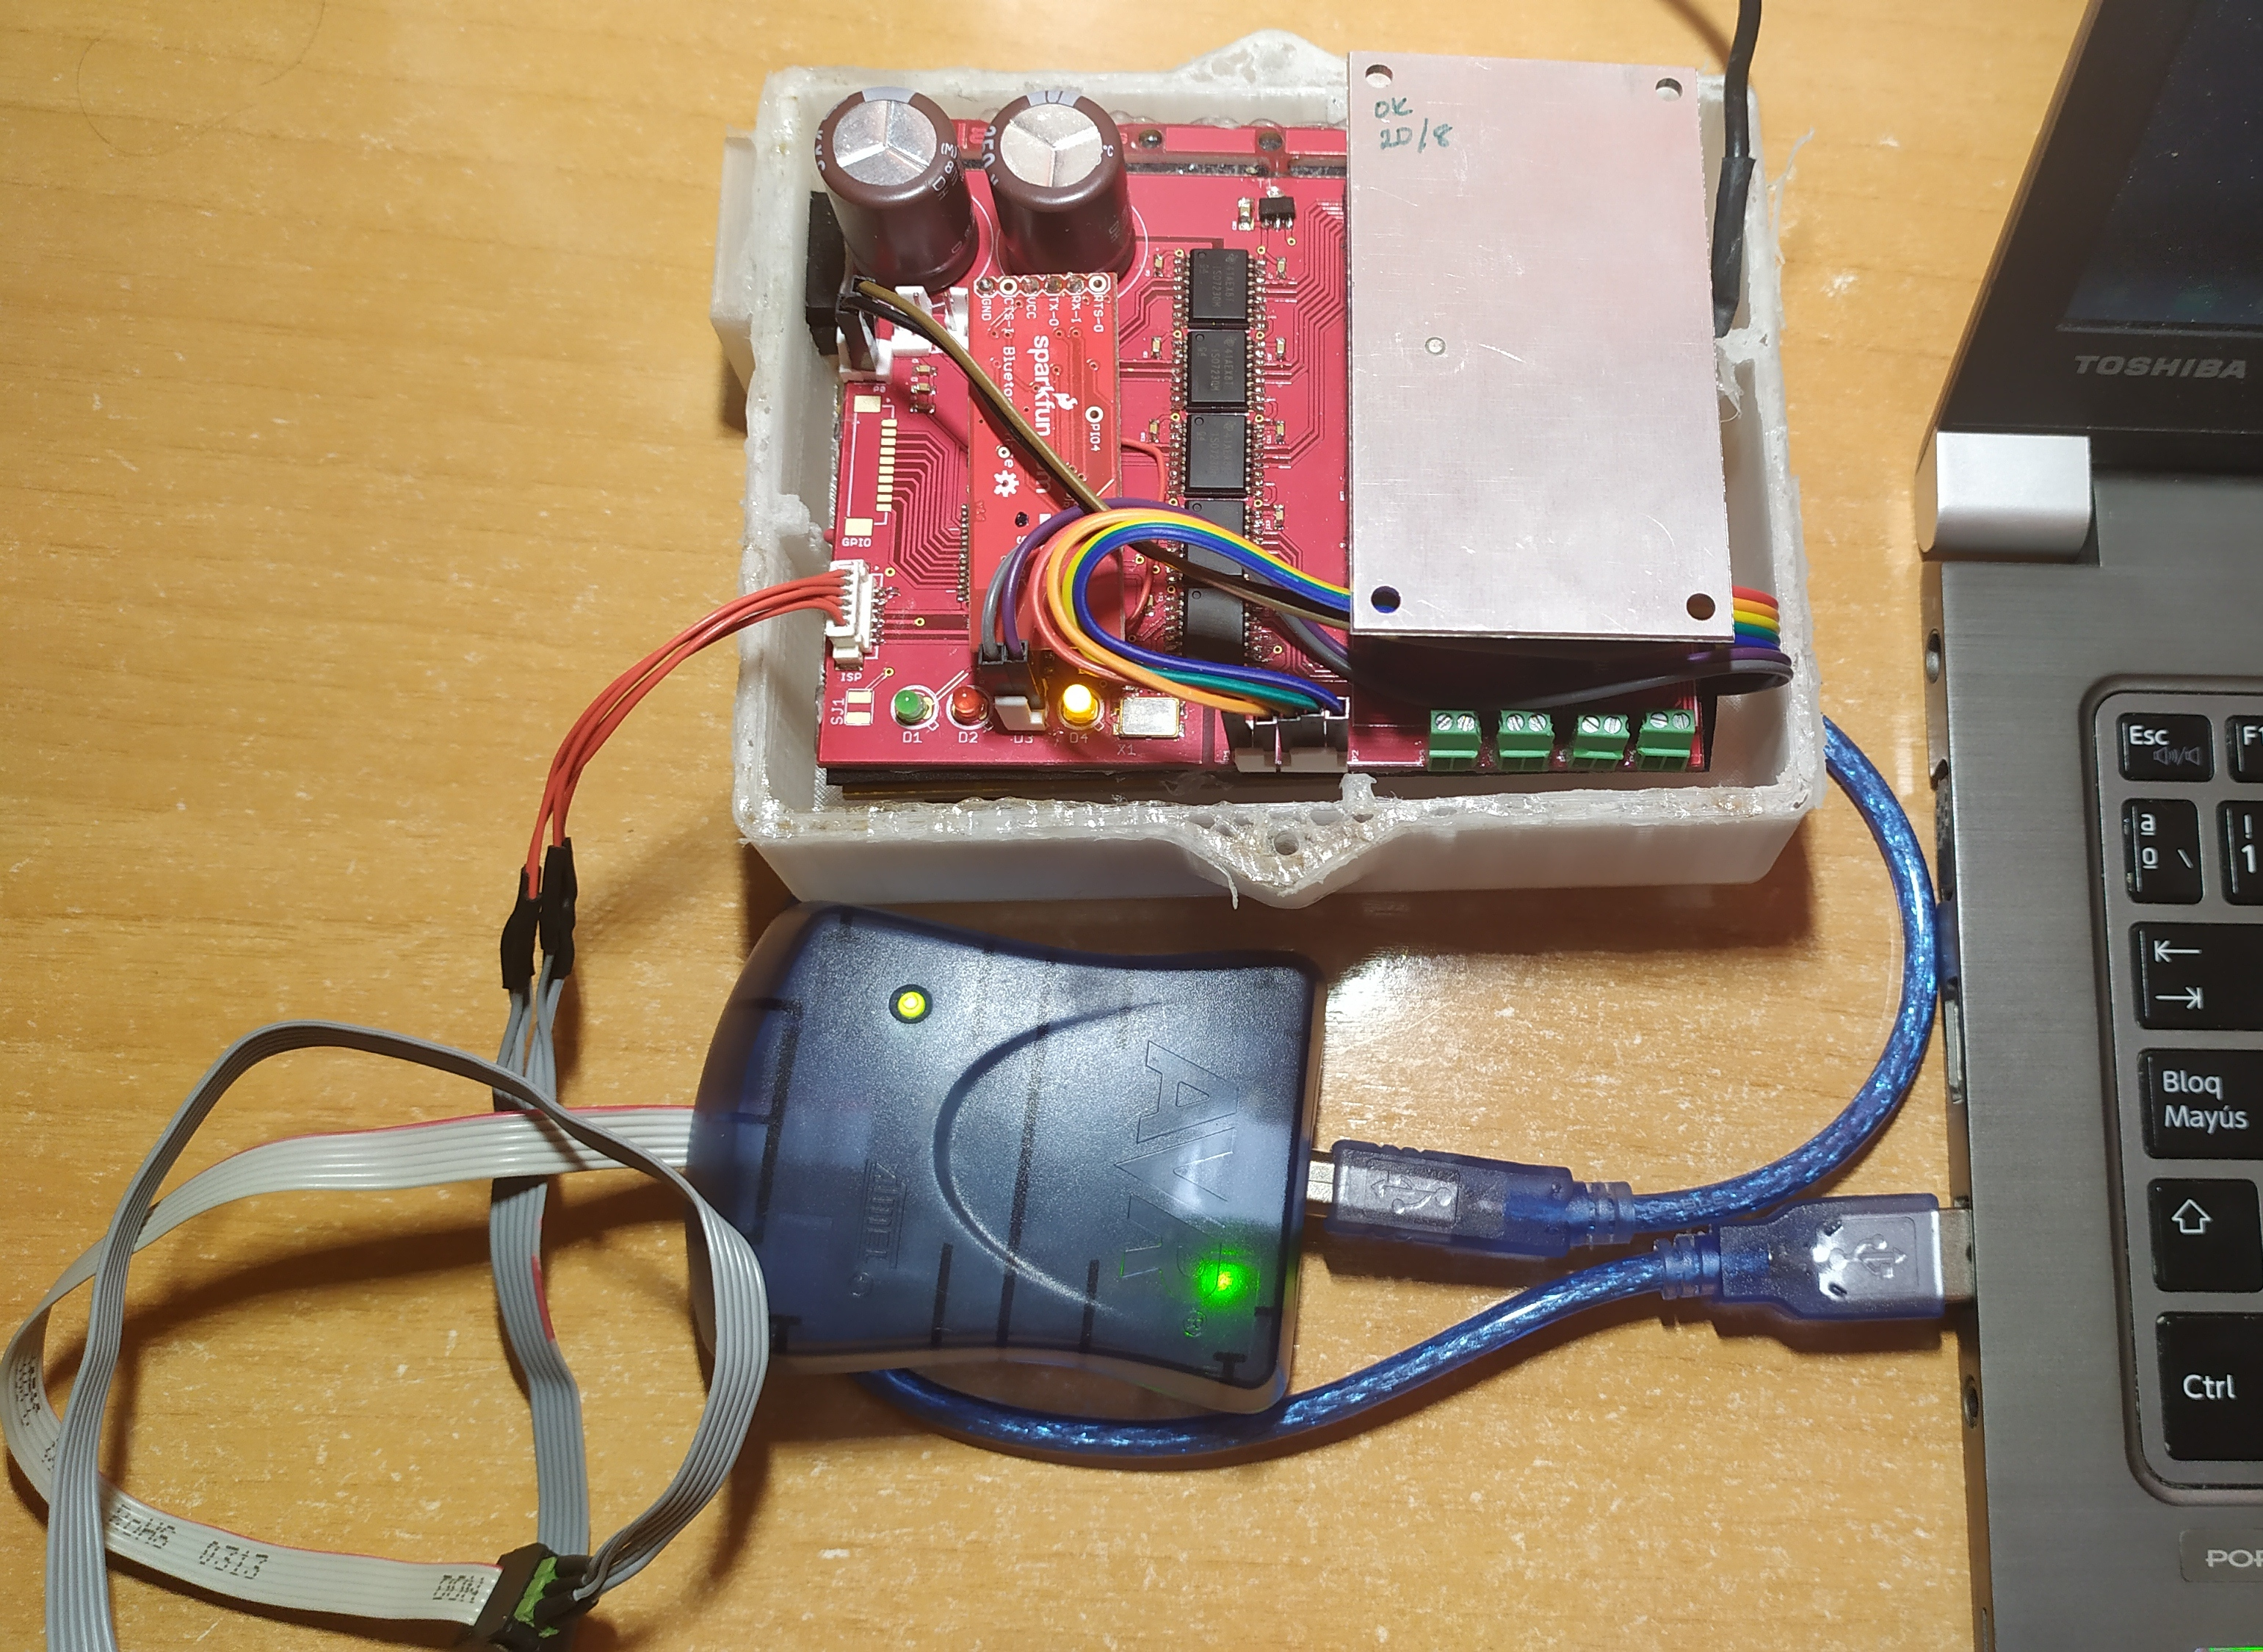
\includegraphics[scale=0.1]{programador_micro}
  \caption{Programador AVRISP mkII conectado al microcontrolador ATmega128 del mini TEREFES mediante ISP.}\label{fig:programador_micro}
\end{figure}

\begin{figure}[!htb]
\centering
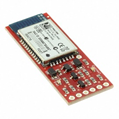
\includegraphics[scale=1.0]{modulo_bluetooth}
  \caption{Módulo Bluetooth Sparkfun Silver Smirf utilizado para la comunicación inalámbirca\cite{modulo_bluetooth}.}\label{fig:modulo_bluetooth}
\end{figure}

\subsection{Montaje}
La etapa de control recibe alimentación de la de potencia mediante los pines P0, P1 y P2 y que se pueden encontrar en su correspondiente esquemático en el Anexo I. En la figura \ref{fig:etapas} se muestra la conexión eléctrica entre las dos etapas del estimulador junto a la batería externa que lo alimenta. De este modo, los pines P0, P1 y P2 de la tarjeta de control que necesitan $5Vdc$, $15Vdc$ y $\pm15Vdc$ respectivamente, quedan unidos por cables a las fuentes de tensión correspondientes en la etapa de potencia.
\\
\\
En cuanto al montaje mecánico, apuntando a la reducción del tamaño del estimulador, sus dos etapas se colocaron enfrentadas por sus reversos separadas por espuma como elemento aislante. A continuación, se fijaron con adhesivo tal y como se aprecia en la figura \ref{fig:placas}.\\

\begin{figure}[!htb]
\minipage{0.5\textwidth}
  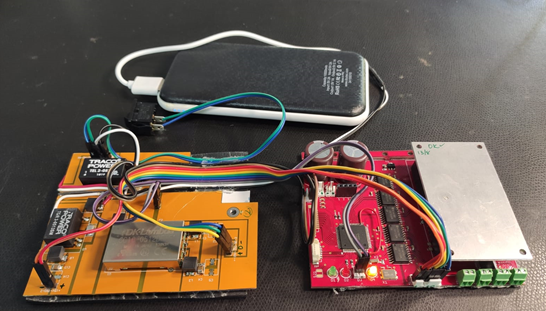
\includegraphics[width=\linewidth]{etapas}
  \caption{Etapas de control (placa roja) y de potencia (placa naranja) junto a la batería portátil que alimenta el estimulador. Los cables que conectan la placa de potencia con la de control proporcionan los niveles de tensión de $5VDC$, $15VDC$ y $\pm15Vdc$ explicados previamente.}\label{fig:etapas}
\endminipage\hfill
\minipage{0.4\textwidth}
  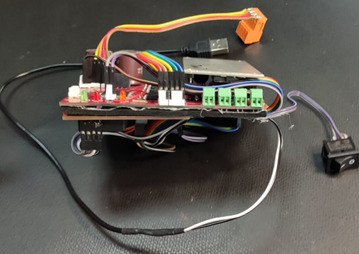
\includegraphics[width=\linewidth]{placas}
  \caption{Montaje de las etapas de control y potencia enfrentando los reversos de sus tarjetas de circuito impreso.}\label{fig:placas}
\endminipage\hfill
\end{figure}

Para contener todos los elementos anteriores se imprimió en 3D una caja para dicho propósito, la cual se muestra en la figura \ref{fig:montaje}. Se tiene además un elemento de sujección para que el estimulador esté fijado al paciente mediante un cinturón tal y como se ve en la figura \ref{fig:montaje_cinturon}.\\

\begin{figure}[!htb]
\centering
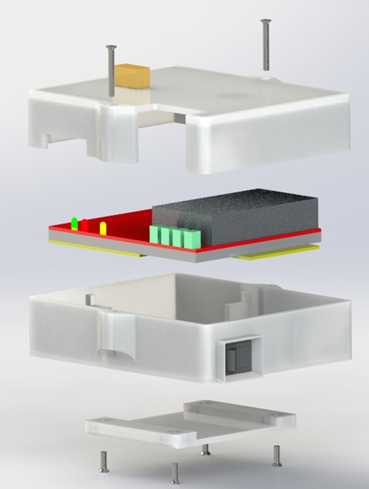
\includegraphics[scale=0.8]{montaje}
  \caption{Montaje del estimulador en la caja impresa en 3D. Desde arriba: tapa superior, etapas de control y potencia, tapa inferior con interruptor de encendido/apagado y elemento de sujección a un cinturón.}\label{fig:montaje}
\end{figure}


\subsection{Firmware}\label{firmware}
El firmware ha sido elaborado en la Universidad Católica de Asunción de Paraguay y permite el control y configuración de los parámetros de la electroestimulación, explicados en el capítulo \ref{capitulo_1} y de acuerdo a las especificaciones de la tabla \ref{tabla:detalles_terefes} mostrada con anterioridad.
\\
\\
Para el control de dichos parámetros, se debe entablar una comunicación entre el estimulador y un ordenador mediante puerto serie ya que se utiliza para enviar diferentes instrucciones. Debido a las capacidades de comunicación inalámbrica que posee el mini TEREFES, se puede establecer conexión con éste haciendo uso de cualquier ordenador que disponga de un módulo Bluetooth. Entonces, una vez completo el proceso de emparejar el dispositivo al ordenador mediante Bluetooth, se abre una terminal de puerto serie (por ejemplo Coolterm\cite{coolterm}) y se establece la conexión con el puerto asociado al estimulador habiendo establecido antes la siguiente configuración:

\begin{itemize}
\item[•] La velocidad de transmisión de datos debe ser de 115200 bits por segundo.
\item[•] La longitud de los mensajes es de 8 bits.
\item[•] Un bit de parada.
\item[•] Modo de paridad deshabilitado.
\item[•] Tras escribir un comando en la terminal, se pulsa la tecla ENTER para enviarlo, acción que el firmware debe detectar como un ``carriage return'' o retorno de carro. Por lo tanto, la acción del ENTER debe ser configurada en la terminal como retorno de carro y no como retorno de carro y nueva línea o line feed.
\end{itemize}

Una vez establecida la conexión, aparecerá en el terminal la línea ``NewCMD:'' devuelta por el dispositivo para indicar la solicitud de entrada de un nuevo comando por teclado. La figura \ref{fig:coolterm_conf} muestra la configuración del terminal descrita previamente.\\  

\begin{figure}[!htb]
\centering
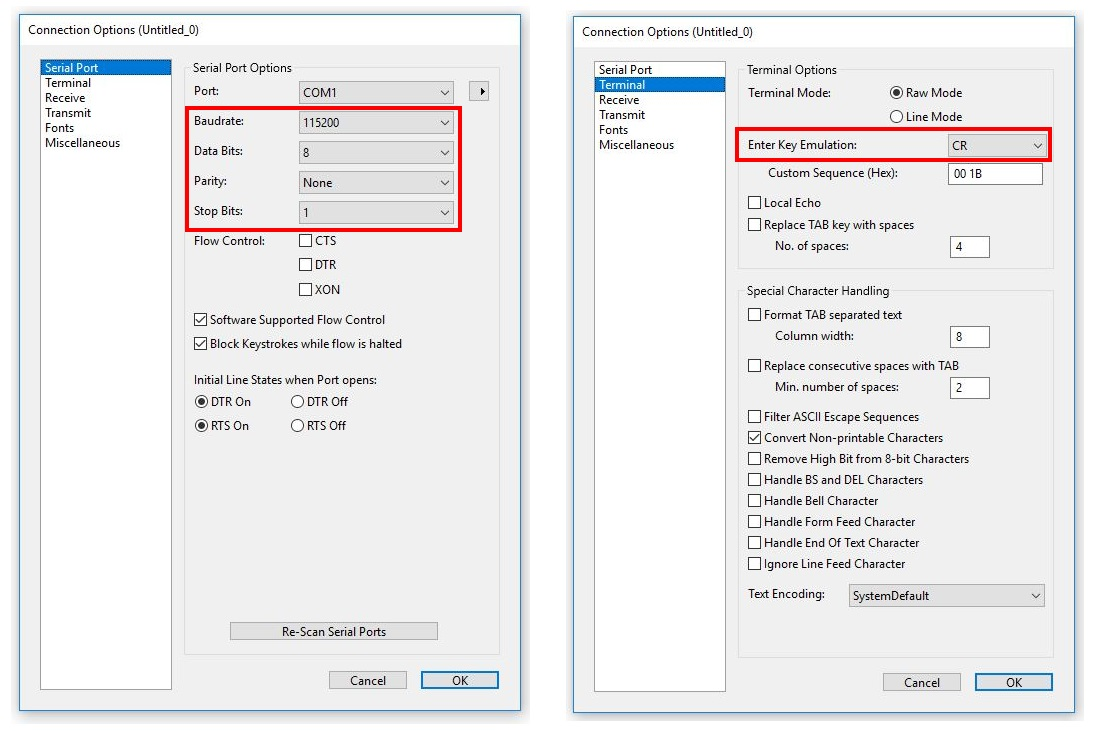
\includegraphics[scale=0.6]{coolterm_conf}
  \caption{Configuración del terminal.}\label{fig:coolterm_conf}
\end{figure}


Para el control del estimulador mediante instrucciones, se ha de considerar en primer lugar si se van a utilizar dos o más canales de estimulación. Si es el caso, se deben configurar los siguientes parámetros que pueden considerarse como los parámetros generales del estimulador:

\begin{itemize}
\item[•] \textbf{Número de canales (fl):} indica el número de canales que debe utilizar el estimulador.
\item[•] \textbf{Lista de canales (lc):} establece el orden de estimulación de los canales, es decir, qué turno tiene cada canal a la hora de estimular ya que un mismo dispositivo no activa dos o más canales a la vez. 
\item[•] \textbf{Frecuencia inter grupo (tg):} indica la frecuencia de repetición de un patrón de estimulación de canales. Debe introducirse en Hz.
\item[•] \textbf{Frecuencia intra grupo (ti):} indica la frecuencia de repetición de la estimulación de un canal dentro de un patrón de estimulación de canales. Debe introducirse en Hz, es decir. La figura \ref{fig:parametros_generales} muestra las frecuencias mencionados.
\end{itemize}

Para configurar o escribir un valor en los parámetros descritos se introduce un comando de la siguiente forma:
$$e\;fl\;[número\;de\;canales\;0-3]$$
$$e\;lc\;[número\;de\;canal\;0-3]\;[turno\;0-3]$$
$$e\;tg\;[frecuencia\;0-255]$$
$$e\;ti\;[frecuencia\;0-255]$$

Se indica entre corchetes el tipo y rango de valores numéricos que debe introducir el usuario por teclado destacando que los valores comienzan en cero y no en uno. Por ejemplo, si se desea utilizar 2 canales siendo el canal 1 el primero en estimular y el canal 2 el segundo en estimular se debe escribir en la terminal:
$$e\;fl\;1$$
$$e\;lc\;0\;0$$
$$e\;lc\;1\;1$$

También es posible leer en el terminal el valor que tienen estos parámetros en el estimulador. Para ello, se deben enviar los siguientes comandos al estimulador para solicitar que transmita el valor de los parámetros especificados:
$$l\;fl$$
$$l\;lc$$
$$l\;tg$$
$$l\;ti$$

\begin{figure}[!htb]
\centering
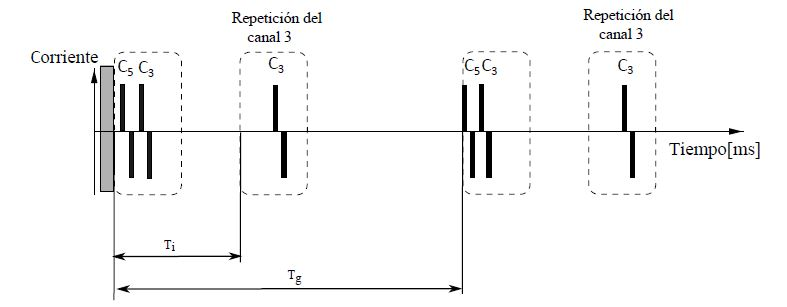
\includegraphics[scale=0.8]{parametros_generales}
  \caption{Frecuencias inter (tg) e intra (ti) grupo sobre un tren de pulsos de corriente. Se muestran en la figura como periodos pero el estimulador trabaja con su inverso, es decir, frecuencia.}\label{fig:parametros_generales}
\end{figure}

Por otra parte, cada canal admite las siguientes configuraciones de parámetros y que pueden quedar definidos como los parámetros de canal:

\begin{itemize}
\item[•] \textbf{Amplitud de corriente:} la amplitud de corriente eléctrica tanto para pulsos positivos (ap) como negativos (an).
\item[•] \textbf{Ancho de pulso:} duración del pulso de corriente positiva (tp) y negativa (tn).
\item[•] \textbf{Repeticiones (re):} repeticiones de estimulación de un canal dentro de un tren de pulsos.
\item[•] \textbf{Inversión de pulso (in):} determina si el primer pulso es positivo o negativo.
\end{itemize}

Para configurar los valores de dichos parámetros se debe introducir el comando correspondiente de la forma:

$$w\;[número\;de\;canal\;0-3]\;ap/an\;[amplitud\;0-115]$$
$$w\;[número\;de\;canal\;0-3]\;tp/tn\;[amplitud\;0-2100]$$
$$w\;[número\;de\;canal\;0-3]\;re\;[repeticiones\;0-3]$$
$$w\;[número\;de\;canal\;0-3]\;in\;[inversión\;0-1]$$

En el primer y segundo comando se debe elegir ap o an. Los valores de inversión de pulso son 0 si se quiere mantener el primer pulso positivo o 1 si se quiere invertir, es decir que el primer pulso sea de corriente negativa.
\\
\\
Por el contrario, si se desea leer todos estos valores asociados a un canal se debe introducir:
$$r\;[número\;de\;canal\;0-3]$$

Por último, existen los siguientes comandos de control:

\begin{itemize}
\item[•] \textbf{Encendido/apagado de tensión de $\pm15Vdc$}. Se ha implementado esta característica para reducir el consumo del electroestimulador. El comando para encender la fuente es $on1$ y para apagarla $off1$.
\item[•] \textbf{Comienzo/detención de la estimulación.} Para comenzar la estimulación se introduce el comando $s$ y para detenerla el comando $p$.
\item[•] \textbf{Modo de operación}. Existen hasta seis modos diferentes en los que puede operar el estimulador. Principalmente determinan cómo se produce la estimulación ya sea de forma continuada, interrumpida y otras variantes para las que no se entrará en más detalle. Se configura un modo de operación con un comando de la forma $e\;md\;[número\;de\;modo\;1-6]$. Si se desea leer el modo configurado se escribe $l\;md$
\item[•] \textbf{Guardado de parámetros.} Mediante el comando $g$ se pueden guardar en la EEPROM del microcontrolador del todos los valores configurados previamente.
\end{itemize}

Se muestra en la figura \ref{fig:coolterm_ejemplo} un ejemplo del control del estimulador en coolterm mediante las instrucciones descritas.\\

\begin{figure}[!htb]
\centering
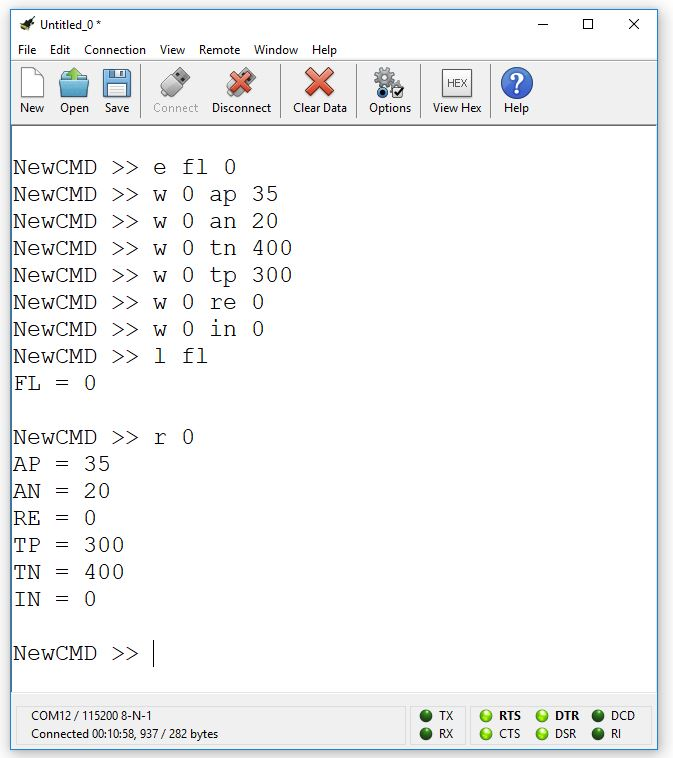
\includegraphics[scale=0.5]{coolterm_ejemplo}
  \caption{Ejemplo de utilización de instrucciones sobre el estimulador eléctrico mediante coolterm.}\label{fig:coolterm_ejemplo}
\end{figure}

Cabe destacar que los valores numéricos correspondientes a los parámetros de corriente (ap y an) ancho de pulso (tp y tn) y frecuencia (tg y ti) no son los reales o físicos, es decir, no son unidades de corriente, tiempo ni frecuencia. Para traducir estos valores a sus correspondientes magnitudes físicas se hace una conversión interna en el estimulador mediante los correspondientes factores de conversión obtenidos empíricamente. Se aprecia en la figura \ref{fig:factores_corriente_ancho} que la relación entre el valor manejado por el estimulador y las magnitudes físicas de intensidad de corriente y ancho de pulso se pueden considerar lineales, por lo que el factor de conversión será una constante. Sin embargo, esto no ocurre con el parámetro de frecuencia cuya función de conversión ha sido deducida tal y como se ve en la figura \ref{fig:factor_frecuencia}.\\

\begin{figure}[!htb]
\centering
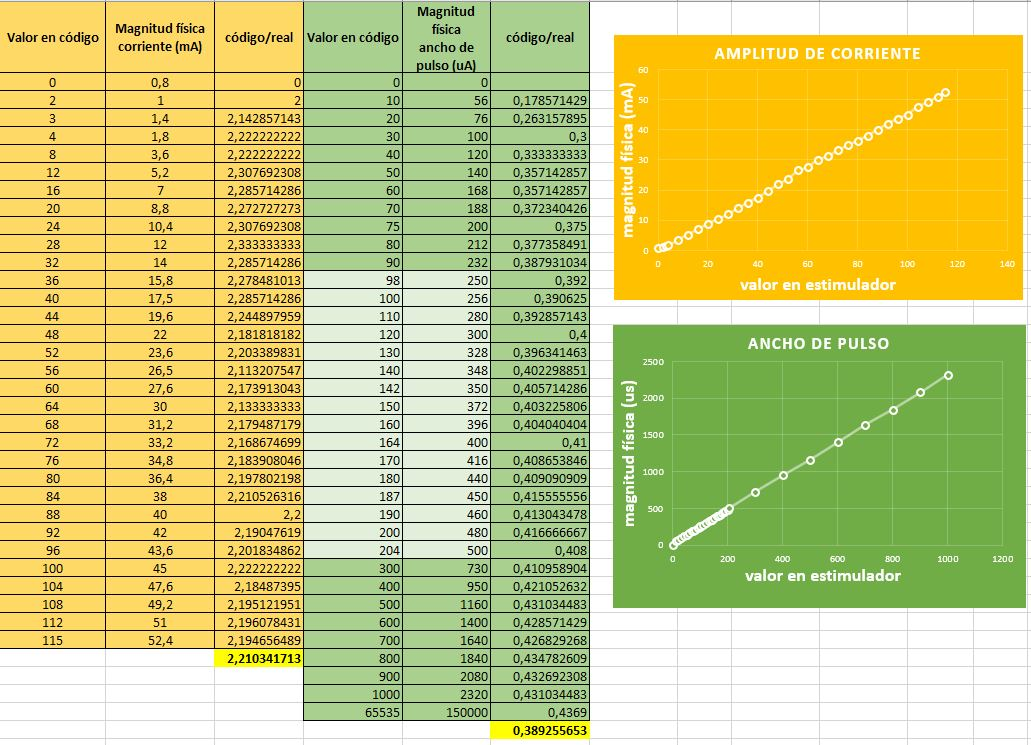
\includegraphics[scale=0.6]{factores_corriente_ancho}
  \caption{Factores de conversión de valores de amplitud de corriente y ancho de pulso manejados por el estimulador. La columna ``valor en código'' es el valor numérico que recibe mediante comandos el estimulador mientras que la columna ``magnitud física'' indica la magnitud física medida mediante un osciloscopio en el canal estiumulado. Los factores de conversión de corriente y ancho de pulso, resaltados en amarillo, se consideran constantes debido a la linealidad de la relación entre el ``valor en código'' y su ``magnitud física''.}\label{fig:factores_corriente_ancho}
\end{figure}

\begin{figure}[!htb]
\centering
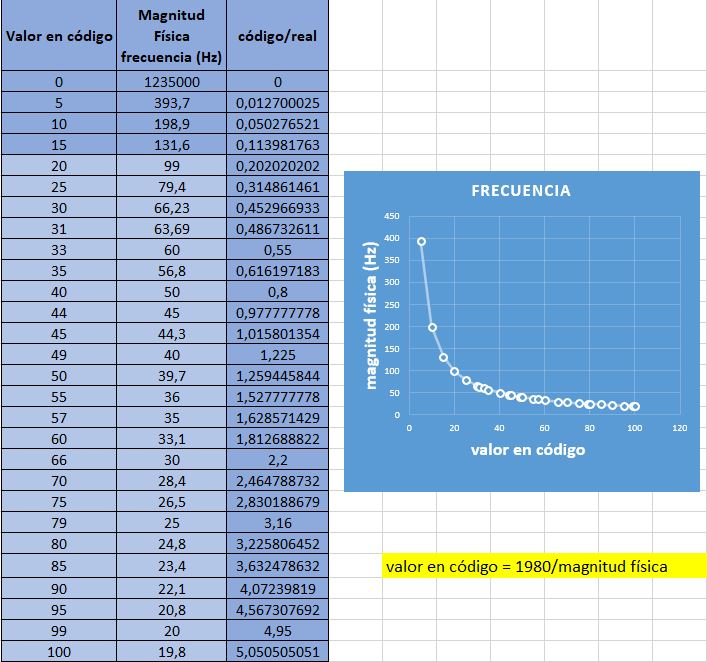
\includegraphics[scale=0.6]{factor_frecuencia}
  \caption{Factor de conversión de la frecuencia de estimulación generada por el estimulador. El ``valor en código'' es el valor numérico que el mini TEREFES recibe mediante comandos mientras que la ``magnitud física'' es la frecuencia medida en Hz en el canal estimulado. Se resalta en amarillo la función aproximada de conversión, deducida a partir del producto de los valores manejados por el estimulador y sus magnitudes físicas, pues se obtiene de forma reiterada un valor de 1980 o muy próximo.}\label{fig:factor_frecuencia}
\end{figure}

No cualquier valor de los parámetros descritos en este apartado (amplitud de corriente, ancho de pulso, frecuencia etc.) son válidos para una electroestimulación adecuada. Para el caso que concierne al proyecto con que se involucra este TFM, es decir, la rehabilitación de la marcha patológica, se consideran principalmente los miembros inferiores del cuerpo. Para estos se tienen unos rangos de valores de los mencionados parámetros mostrados a continuación:

\begin{itemize}
\item[•] \textbf{Amplitud de corriente:} La corriente inducida sobre el paciente a través de los parches adecuados tiene un valor mínimo de 0 $mA$ (no hay estimulación) y un valor máximo de 50 $mA$ (valores tan altos como el mencionado se utilizan solamente sobre músculos grandes como el cuádriceps).
\item[•] \textbf{Ancho de pulso:} el ancho de pulso oscila entre 250 y 500 $\mu s$.
\item[•] \textbf{Frecuencias inter e intra pulso:} la frecuencia de estimulación puede tomar valores tan bajos como 20$Hz$ y un valor máximo de 100$Hz$.
\end{itemize} 

Por último, se ha de tener en cuenta que la manera en la que se establecerá comunicación con los estimuladores desde el exterior es mediante la interfaz gráfica de usuario que se pretende implementar en el presente trabajo. Para ello, se integrarán en la misma las instrucciones de control ya explicadas. Además, se debe contrarrestar la conversión interna de parámetros previamante explicada para que al introducir, por ejemplo, $30mA$ como corriente de estimulación efectivamente se obtengan $30mA$ en el canal correspondiente y no otro valor.

\section{Exoesqueleto robótico}
Poner todas la especificaciones indicadas en los mails , control de posicion, par, velocidad, perfiles de movimiento etc.


\section{Sensores}
Se va a utilizar una serie de sensores para obtener más información sobre el ciclo de la marcha efectuado por el paciente así como del estado de la propia prótesis.

\subsection{Electrogoniómetros}
Para medir el ángulo de flexión de rodillas, tobillos y caderas se utilizan los electrogoniómetros desarrollados por Biometrics\cite{goniometros}. Estos sensores son capaces de medir ángulos de hasta $180\degree$ en los dos ejes perpendiculares al dispositivo, a su vez perpendiculares entre ellos, con una resolución de $0.1\degree$. Son inalámbricos y pueden trabajar hasta una distancia de $30m$ del dispositivo de recolección de datos conectado por USB a un ordenador. Cada goniómetro tiene dos canales de comunicación arrojando cada uno de ellos medidas de ángulos y demás datos referidos a uno de los dos ejes espaciales en los que efectúa dichas mediciones. La tabla \ref{fig:goniometros_specs} muestra las características de los diferentes modelos y en la figura \ref{fig:goniometros} una fotografía de los dos modelos de los que se dispone. 
\\
\\
La forma en la que se colocan estos sensores sobre el paciente se aprecia en la figura \ref{fig:goniometros_setup}. Normalmente el sensor queda fijado con cinta de doble cara a la piel pero se puede añadir cinta adhesiva alrededor de la extremidad para sujetarlo firmemente.\\

\begin{figure}[!htb]
\centering
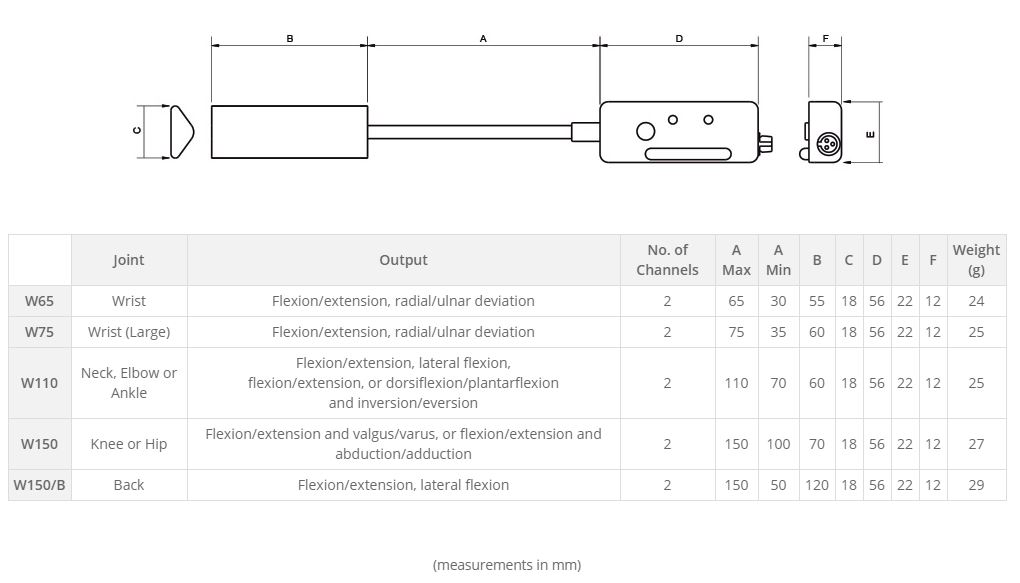
\includegraphics[scale=0.65]{goniometros_specs}
  \caption{Especificaciones de los electrogoniómetros de Biometrics\cite{goniometros}. Se dispone de dos unidades del modelo W110 y cuatro unidades del W150.}\label{fig:goniometros_specs}
\end{figure}


\begin{figure}[!htb]
\centering
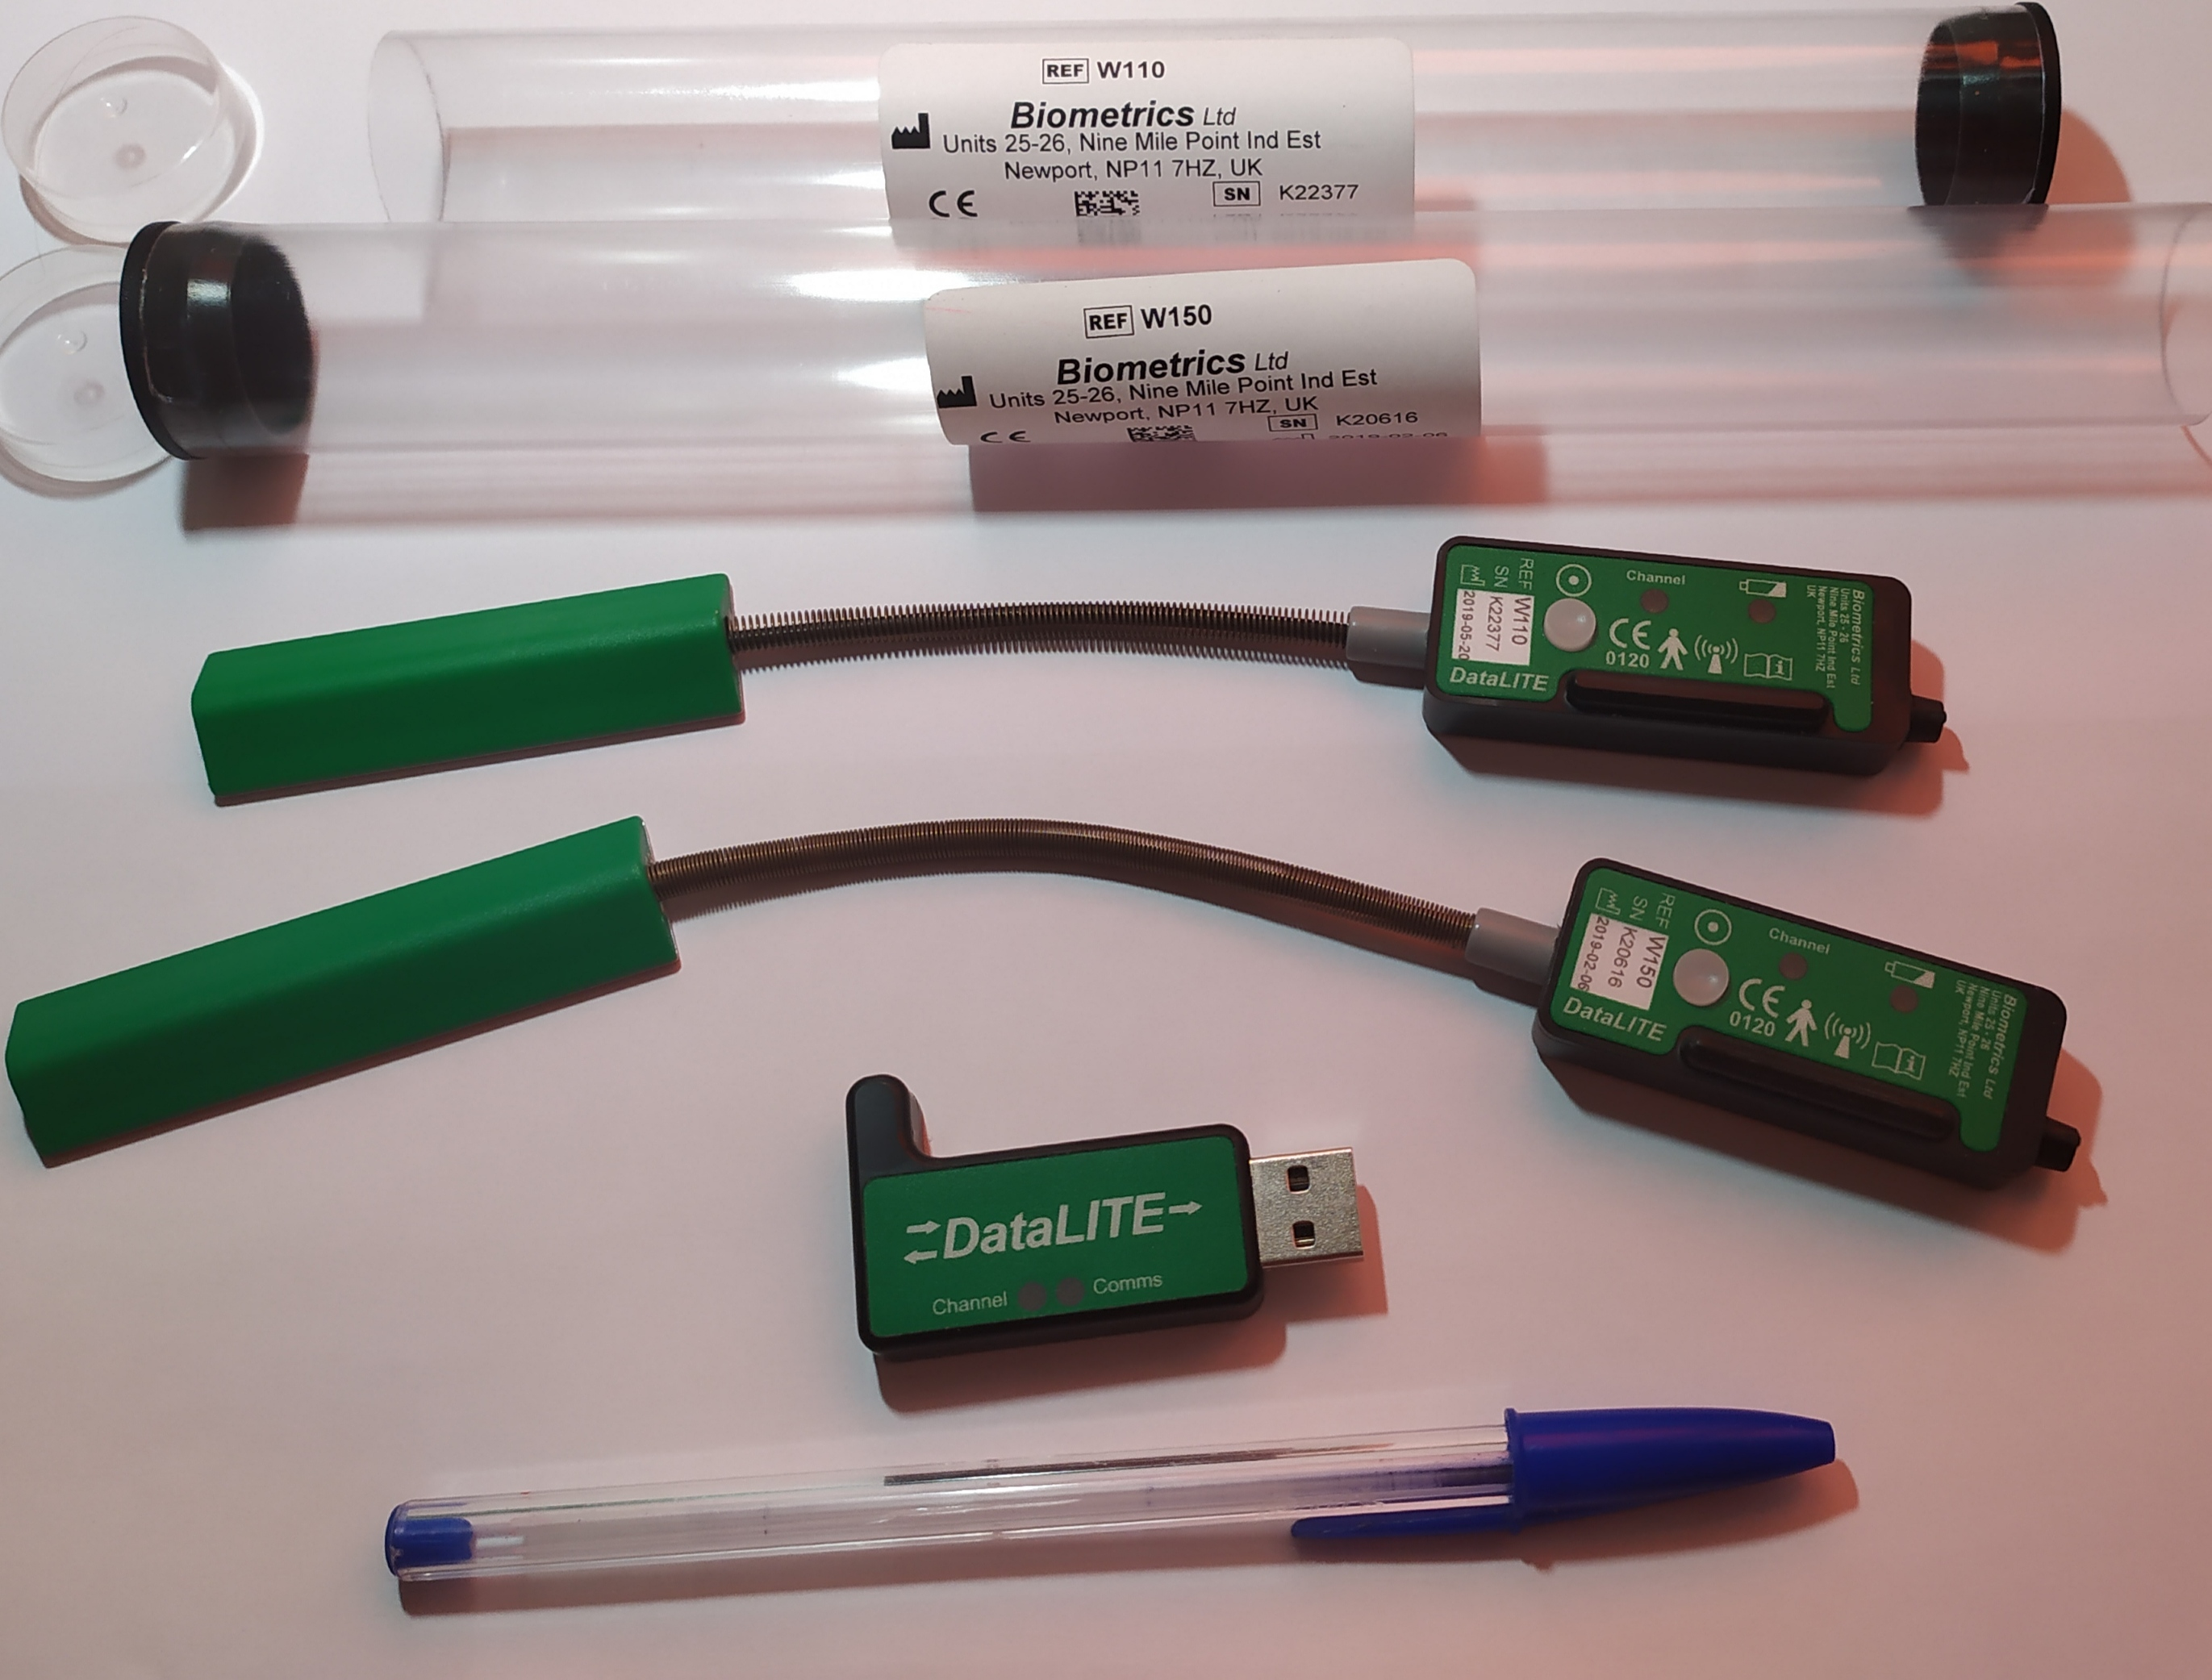
\includegraphics[scale=0.10]{goniometros}
  \caption{Electrogoniómetros W150 (grande) y W110 (pequeño) junto al receptor inalámbico de datos con conexión USB.}\label{fig:goniometros}
\end{figure}


\begin{figure}[!htb]
\centering
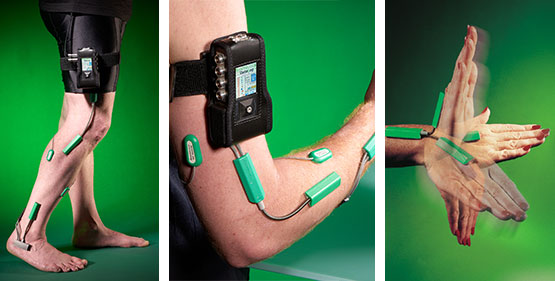
\includegraphics[scale=0.5]{goniometros_setup}
  \caption{Colocación de goniómetros sobre el paciente\cite{goniometros_setup}.}\label{fig:goniometros_setup}
\end{figure}

Junto al hardware, se dispone de la aplicación desarrollada por Biometrics para poder hacer uso de estos sensores y recolectar los datos deseados a través del receptor USB mencionado previamente. Se muestra este software en la figura \ref{fig:data_log}.\\

\begin{figure}[!htb]
\centering
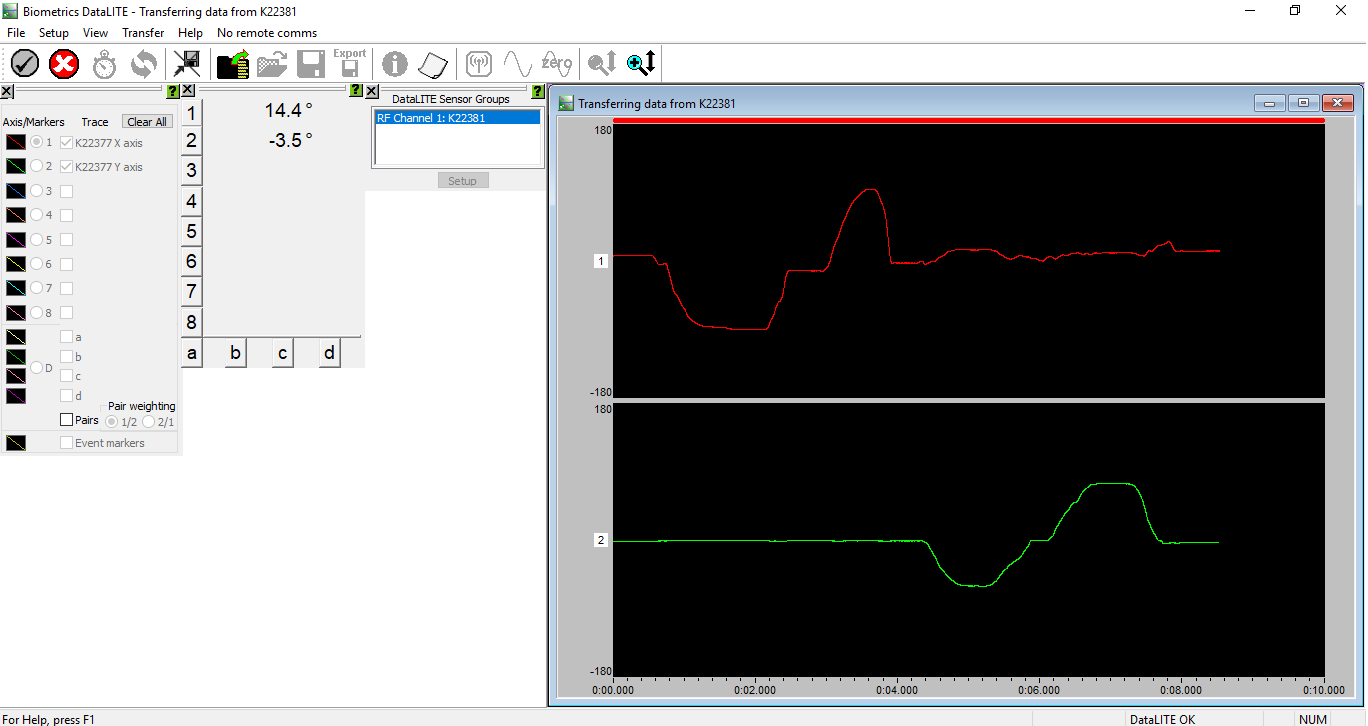
\includegraphics[scale=0.4]{data_log}
  \caption{Interfaz de Biometrics para recogida y disposición de datos de los goniómetros. Se aprecian dos gráficas, una para cada canal de un sólo goniómetro, es decir, medidas de ángulos en dos ejes perpendiculares.}\label{fig:data_log}
\end{figure}

En cuanto al funcionamiento de estos dispositivos, se diferencian dos formas de hacer uso de los mismos y obtener las mediciones de ángulos durante la ejecución del ejercicio de rehabilitación:
\begin{itemize}
\item[•] \textbf{Método directo:} implica utilizar las herramientas básicas de hardware y software ofrecidas por Biometrics. De este modo, se colocan sobre el paciente los goniómetros y se encienden pulsando el botón blanco que hay en ellos. A continuación, se conecta a un ordenador el receptor USB y se abre la aplicación de Biometrics. De acuerdo a la guía de usuario de dicha aplicación, se configura el número de goniómetros utilizados, el canal que le corresponde a cada uno y demás aspectos de configuración. Una vez dispuesto todo lo anterior, se pulsa sobre el botón de la aplicación que permite el comienzo de recepción de datos mientras se muestran en tiempo real en sus correspondientes gráficas. Cuando termina la sesión, es posible guardar en un archivo los datos de la misma.

\item[•] \textbf{Método indirecto:} implica la capacidad de recibir las mediciones de los goniómetros en una aplicación independiente y externa a Biometrics y que puede ser desarrollada por el usuario. Para ello, se debe entender cómo funciona la comunicación entre los sensores y el ordenador al que envían mediciones. Cuando se inicia en el ordenador la aplicación de Biometrics, ésta genera un espacio reservado de memoria en forma de buffer al cual le llega información de los sensores mediante el receptor USB. En el método directo, la aplicación coge estas mediciones del buffer pero en el método indirecto se pueden sacar estos datos sin necesidad de utilizar el software de Biometrics. Para ello, se dispone de unas bibliotecas de vínculos dinámicos (Dynamic-link library o DLL) que fueron entregadas por Biometrics. Estas bibliotecas contienen una serie de funciones que permiten obtener la información disponible en el buffer previamente descrito y por lo tanto hacer uso de la misma en una aplicación independiente al software de Biometrics. La figura \ref{fig:biometrics} muestra de forma esquemática el método indirecto de uso de los goniómetros.
\end{itemize}

\begin{figure}[!htb]
\centering
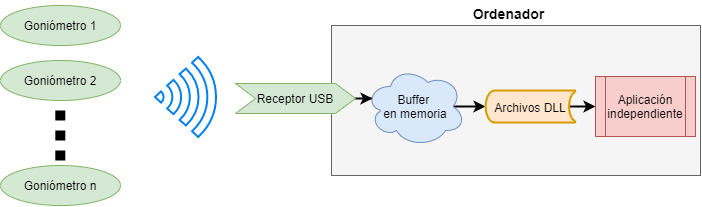
\includegraphics[scale=0.6]{biometrics}
  \caption{Proceso de transmisión de datos desde los goniómetros hasta una aplicación independiente mediante las bibliotecas aportadas por Biometrics}\label{fig:biometrics}
\end{figure}

Las bibliotecas mencionadas en el método indirecto permiten acceder a diferentes tipos de mediciones o parámetros de configuración de los goniómetros para cada uno de sus dos canales. De este modo, es posible obtener la frecuencia de muestreo así como el número de muestras disponibles en el buffer para ser leídas. Además, es posible obtener una estructura de datos que contiene un vector con las mediciones de ángulos efectuadas por el sensor. Por último, en el caso de producirse algún error, éste se refleja en los valores leídos del buffer por lo que se tiene control externo sobre lo que ocurre en los goniómetros. Es por tanto el método indirecto el ideal para hacer uso de los goniómetros en la interfaz de usuario que se pretende realizar en el presente trabajo, siendo ésta la aplicación independiente mencionada en este tipo de control. Se aprecia esta configuración en la figura \ref{fig:configuracion_actual}.\\

\begin{figure}[!htb]
\centering
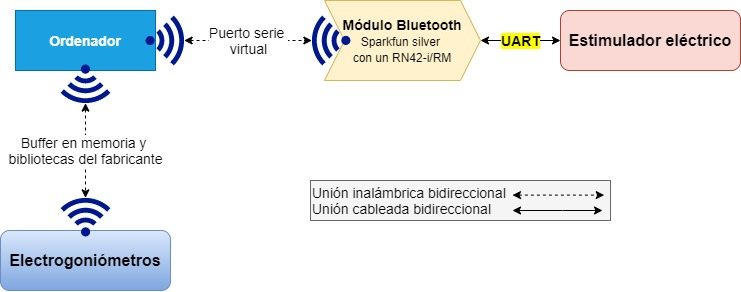
\includegraphics[scale=0.6]{configuracion_actual}
  \caption{Configuración para el control de un electroestimulador y el conjunto de goniómetros desde un ordenador.}\label{fig:configuracion_actual}
\end{figure}






\chapter{Mejora del hardware de los electroestimuladores}
El presente capítulo se centra en el estudio y mejora del hardware de los estimuladores eléctricos de la prótesis híbrida. Se plantea este capítulo con el objetivo principal de obtener un electroestimulador robusto, ligero y de tamaño reducido.
\\
\\
Se identificará en primer lugar el conjunto de objetivos de mejora del mencionado dispositivo que servirán de guía para el planteamiento de tareas enfocadas a mejorar su hardware. 
\\
\\
Por último, se expondrá el cumplimiento de dichas tareas así como la validación de objetivos para mostrar en efecto una mejora en el hardware del electroestimulador.

\section{Etapa de potencia}\label{mejora_hardware_potencia}
La etapa de potencia del electroestimulador es la que más trabajo necesita en cuanto a tareas de mejora. Se va a explicar en este apartado el conjunto de características de la misma así como los motivos para efectuar una mejora sustancial en ésta. 

\subsection{Revisión del hardware y planteamiento de objetivos de mejora}
Tal y como se explicó en el estudio de la prótesis híbrida realizado en el apartado \ref{etapa_potencia} del capítulo \ref{capitulo_2}, la etapa de potencia del electroestimulador pertenece a una versión anterior del mismo llamada TEREFES. Esta etapa reciclada dispone de los siguientes elementos los cuales se pueden ver en la figura \ref{fig:fuente_terefes}:

\begin{itemize}
\item[•] Entrada de $5Vdc$ desde una batería externa.
\item[•] Una fuente de $5Vdc$ implementada con un convertidor de corriente continua. Su entrada son los $5Vdc$ de la batería y su salida son $5Vdc$. Además, se utilizan diferentes componentes pasivos.
\item[•] Dos fuentes de $15Vdc$ y $\pm15Vdc$ implementadas con dos convertidores de corriente continua de $5Vdc$ a $15Vdc$ y $5Vdc$ a $\pm15Vdc$ respectivamente. Se tienen también diferentes componentes pasivos. La entrada de $5Vdc$ de los convertidores procede de la batería.
\end{itemize}

Sin embargo, el electroestimulador utilizado en la prótesis híbrida no necesita una de las fuentes de $15Vdc$ y $\pm15Vdc$ lo cual se aprecia en la figura \ref{fig:fuente_mini_terefes}. Esto implica que el montaje de la etapa de potencia del mini TEREFES requiere recortar una de las placas de circuito impreso de la etapa de potencia del TEREFES de la forma mostrada en la figura \ref{fig:potencia_recorte}. En esta figura, el cable negro superior conecta las masas de los recortes de la placa mientras que el cable rojo superior conecta su alimentación de $5Vdc$ desde una batería externa. Los cables rojo y negro inferiores sirven para el encendido y apagado del convertidor de $\pm15Vdc$ desde el microcontrolador de la etapa de control. 
\\
\\
Por otra parte, las salidas de las fuentes de tensión alimentan la etapa de control mediante cables del tipo ``jumper'' que conectan los correspondientes puntos de ambas placas mediante pines montados ``through hole''. Dichos pines son los que llevan los niveles de tensión mencionados previamente así como las referencias de masa de cada fuente. De este modo, la fuente de $5Vdc$ tiene dos pines a su salida, los $5Vdc$ y su referencia a masa. La fuente de $15Vdc$ dispone así mismo de dos pines en su salida, el que aporta el nivel de tensión mencionado y la referencia a masa. Por último, la fuente de $\pm15Vdc$ tiene tres pines en su salida y que corresponden a los niveles de tensión de $15Vdc$, $-15Vdc$ y su referencia a masa. Tanto el montaje de las tarjetas de control y potencia como su conexión eléctrica se muestra en las figuras \ref{fig:etapas} y \ref{fig:placas}.
\\
\\
Además, el tamaño de la tarjeta de la etapa de potencia no es todo lo compacta posible debido a su procedencia. En un aplicación como en la que se involucra el presente Trabajo Fin de Máster, el tamaño y por tanto peso y volumen de los componentes de la prótesis híbrida es un factor de vital importancia. Se pretende llevar a cabo un asistencia al paciente de la forma menos invasiva posible. En este caso, se desea reducir el tamaño de la etapa de potencia y por tanto del estimulador eléctrico ya que el paciente llevará puestos hasta cuatro de estos dispositivos.\\

\begin{figure}[!htb]
\minipage{0.45\textwidth}
  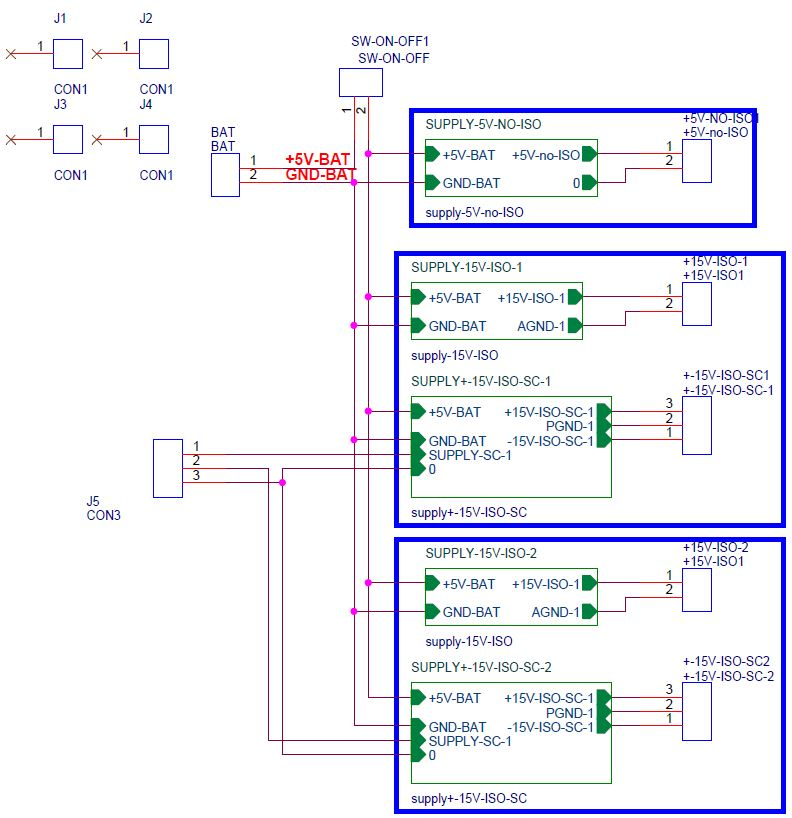
\includegraphics[width=\linewidth]{fuente_terefes}
  \caption{Esquemático de la etapa de potencia del TEREFES con alimentación a $5Vdc$ de la batería (BAT), una fuente de $5Vdc$ en cuadro el azul superior y dos fuentes de $15Vdc$ y $\pm15Vdc$, cada una de ellas en los dos cuadros azules inferiores.}\label{fig:fuente_terefes}
\endminipage\hfill
\minipage{0.45\textwidth}
  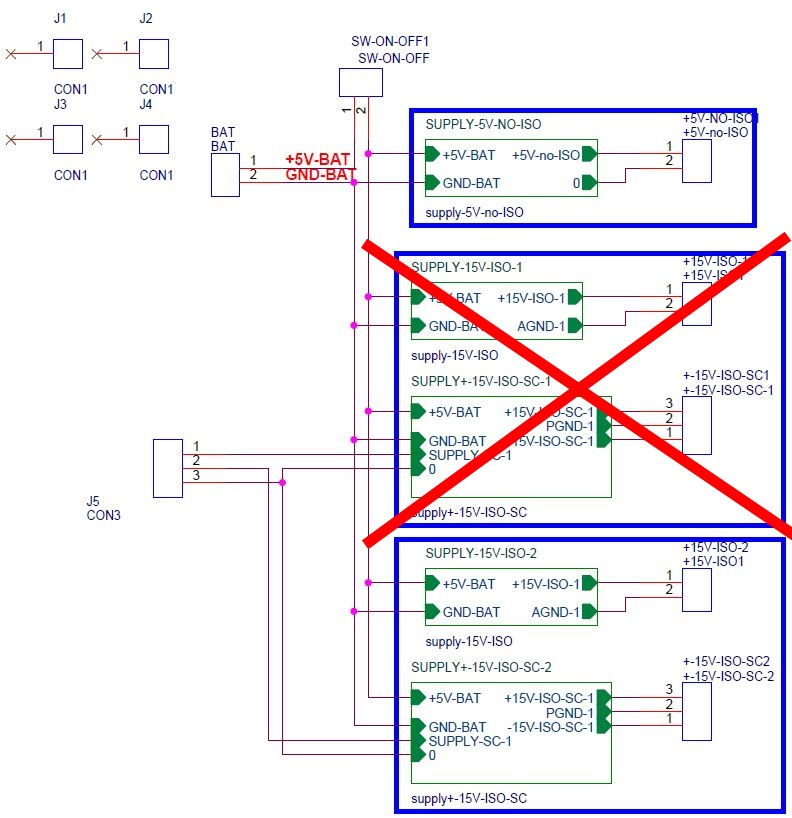
\includegraphics[width=\linewidth]{fuente_mini_terefes}
  \caption{Esquemático de la etapa de potencia del mini TEREFES con una fuente de $5Vdc$ y otra de $15Vdc$ y $\pm15Vdc$.}\label{fig:fuente_mini_terefes}
\endminipage\hfill
\end{figure}

\begin{figure}[!htb]
\centering
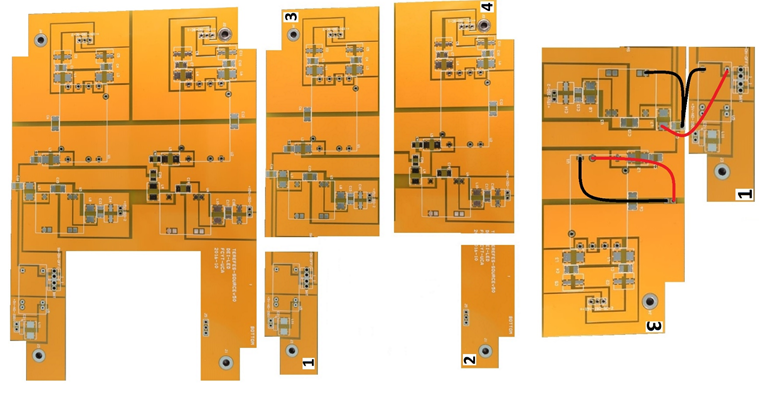
\includegraphics[scale=0.7]{potencia_recorte}
  \caption{Adapatación de la etapa de potencia reciclada del estimulador TEREFES. A la izquierda se tiene la etapa de potencia original. En el centro se muestran los cortes efectuados y los bloques resultantes numerados. A la derecha se conectan los bloques 1 y 3 necesarios para la etapa de potencia del mini TEREFES que contienen la fuente de $5Vdc$ y las fuente de $15Vdc$ y $\pm15Vdc$ respectivamente.}\label{fig:potencia_recorte}
\end{figure}

\begin{figure}[!htb]
\minipage{0.5\textwidth}
  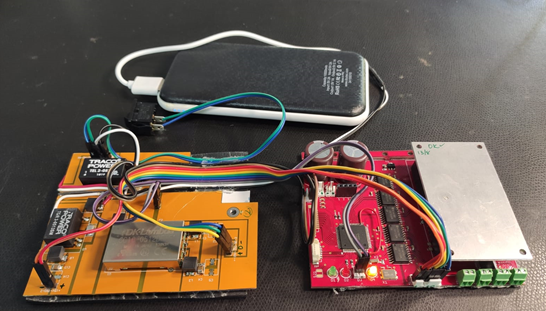
\includegraphics[width=\linewidth]{etapas}
  \caption{Etapas de control (placa roja) y de potencia (placa naranja) junto a la batería portátil que alimenta el estimulador. Los cables que conectan la placa de potencia con la de control proporcionan los niveles de tensión de $5Vdc$, $15Vdc$ y $\pm15Vdc$.}\label{fig:etapas}
\endminipage\hfill
\minipage{0.4\textwidth}
  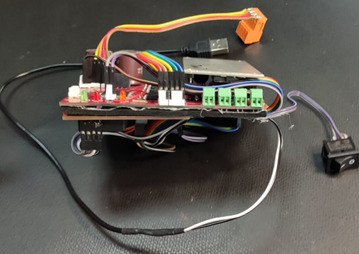
\includegraphics[width=\linewidth]{placas}
  \caption{Montaje enfrentado de las etapas de control y potencia.}\label{fig:placas}
\endminipage\hfill
\end{figure}

Se identifica en este punto un problema de tamaño e integridad de la etapa de potencia del mini TEREFES ya que se está utilizando una tarjeta de circuito impreso que no ha sido diseñada específicamente para este electroestimulador. Además, las placas de potencia y control están unidas eléctricamente mediante jumpers, los cuales no son ideales en conexiones que deben ser fiables. Es más, el estimulador va sujeto en el paciente durante ejercicios de rehabilitación que implican movimiento y manipulación del dispositivo para su puesta a punto y correcta colocación. 
\\
\\
Por lo tanto, aunque el dispositivo es funcional existen vías de mejora en cuanto a su etapa de potencia. De este modo, una vez comprendido el estado del mini TEREFES en cuanto a dicha etapa, se plantea el rediseño de la misma de modo que se fijan los siguientes objetivos:

\begin{itemize}
\item[\textbf{1)}] Reducción y optimización del tamaño y forma de la tarjeta de circuito impreso de la etapa de potencia. Ésta se adaptará al tamaño y forma de la tarjeta de control.
\item[\textbf{2)}] Alineamiento de las salidas de las fuentes de tensión de la etapa de potencia con los puntos de la etapa de control que requieren esta alimentación. Se parte del la idea de que el montaje de las placas de control y potencia se efectúa enfrentando sus reversos según se muestra en la figura \ref{fig:placas}. Se pretende entonces situar las salidas de los convertidores en la placa de potencia de manera que al efectuar el montaje mencionado previamente, queden alineadas con los puntos de la placa de control que necesitan esta alimentación. Esta conexión es posible porque tanto las salidas de las fuentes de la placa de potencia como los puntos de la placa de control que conectan con los anteriores, son agujeros en sus tarjetas de circuito impreso correspondientes. Esto implica que dichos puntos se pueden conectar mediante pines soldados a los agujeros mencionados. Se explica en las figuras \ref{fig:montaje_alineado} y \ref{fig:montaje_alineado_seccion} este objetivo.\\

\begin{figure}[!htb]
\centering
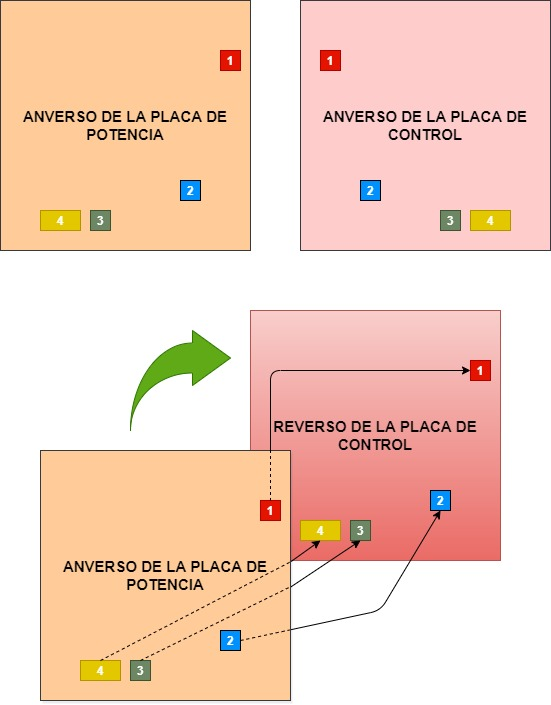
\includegraphics[scale=0.5]{montaje_alineado}
  \caption{Representación del montaje alineado de las placas de potencia y control. En la parte superior se disponen ambas placas por su anverso. En la parte inferior se ha volteado horizontalmente la placa de control y se coloca sobre ésta la placa de potencia, de modo que los reversos quedan enfrentados. Los cuadros 1, 2, 3 y 4 son las conexiones de ambas placas que se desean alinear: la conexión 1 es la salida de $5Vdc$ del correspondiente convertidor de la etapa de potencia y el punto que requiere esta tensión en la placa de control. La conexión 2 es el control remoto para el encendido y apagado del convertidor de $\pm15Vdc$ efectuado desde el microcontrolador de la placa de control. Por último, las conexiones 3 y 4 son las salidas de los convertidores de $15Vdc$ y $\pm15Vdc$ respectivamente y que aportan este nivel de tensión a los correspondientes puntos de la placa de control. Las conexiones 1, 2 y 3 necesitan dos pines mientras que la 4 necesita tres, tal y como se ha explicado con aterioridad.}\label{fig:montaje_alineado}
\end{figure}

\begin{figure}[!htb]
\centering
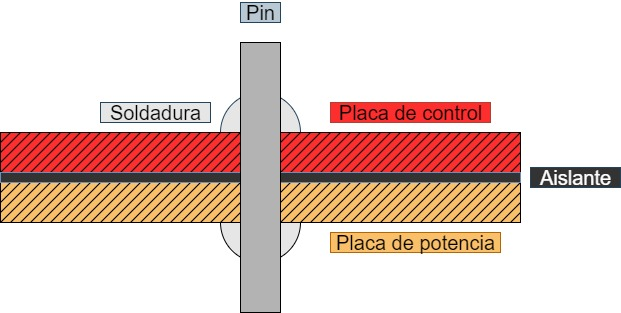
\includegraphics[scale=0.5]{montaje_alineado_seccion}
  \caption{Representación de la sección del montaje alineado de las placas del mini TEREFES. El pin representa la unión soldada de las placas entre los puntos correspondientes de las placas de control y potencia.}\label{fig:montaje_alineado_seccion}
\end{figure}

\end{itemize}

\subsection{Rediseño de la etapa de potencia}
La mejora de la etapa de potencia del mini TEREFES se realiza con Eagle\cite{eagle}, un software de diseño asistido por computador para la realización de esquemáticos de circuitos electrónicos y tarjetas de circuito impreso. Se ha elegido este software debido a que la etapa de control del electroestimulador se ha creado con el mismo, de modo que el principal motivo para dicha elección es la homogeneidad en diseños electrónicos de este componente de la prótesis híbrida. Además, el autor del presente trabajo dispone de licencia de estudiante de Autodesk, compañía propietaria de Eagle.

\subsubsection{Esquemático}
Se parte del diseño original de la etapa de potencia, es decir del TEREFES, dispositivo del que procede el estimulador eléctrico de la prótesis híbrida, el mini TEREFES. Este diseño, tal y como se ha descrito con anterioridad, dispone de una entrada de $5Vdc$ desde una batería externa, una fuente de $5Vdc$ y dos fuentes de $15Vdc$ y $\pm15Vdc$. En la figura \ref{fig:fuente_terefes} mostrada anteriormente se aprecia un esquemático a alto nivel de esta etapa mientras que en las figuras \ref{fig:fuente5vdc_esquematico}, \ref{fig:fuente15vdc_esquematico} y \ref{fig:fuente+-15vdc_esquematico} del Anexo II se muestra en mayor detalle el esquemático de cada fuente de tensión. 
\\
\\
Se toman entonces los componentes mostrados en estas figuras y se crea en Eagle el esquemático de la nueva etapa de potencia del mini TEREFES. Sin embargo, Eagle y como otros programas para diseño de circuitos electrónicos disponen de unas bibliotecas limitadas. Esto implica que en este caso Eagle no tiene el símbolo ni la huella de los siguientes componentes:

\begin{itemize}
\item[•] Convertidor de $5Vdc$ a $5Vdc$ TEL 2-0511\cite{convertidor_5vdc}.
\item[•] Convertidor de $5Vdc$ a $15Vdc$ TDR 3-0513SM\cite{convertidor_15vdc}.

\end{itemize}

Se ha generado una biblioteca en Eagle en la que almacenar los símbolos y huellas que el autor del presente trabajo ha creado para estos componentes siguiendo las indicaciones de sus hojas de datos. El resto de componentes se encontraban en las bibliotecas de Eagle o bien sus huellas y símbolos ya existían, las cuales se pueden encontrar en páginas web como snapeda\cite{snapeda} y se pueden importar a la biblioteca mencionada.
\\
\\
En el caso del convertidor TEL 2-0511 se parte de su hoja de datos mostrada en la figura \ref{fig:convertidor_5vdc_datasheet}. Con ella se generan en Eagle un símbolo y una huella los cuales se aprecian en las figuras \ref{fig:convertidor_5vdc_simbolo} y \ref{fig:convertidor_5vdc_huella} respectivamente. Por otra parte, se toma la hoja de datos del convertidor TDR 3-0513SM para crear su símbolo y huella en Eagle. para el caso de la huella, la hoja de datos proporciona una recomendación que se ha implementado de la misma forma. Se muestra en las figuras \ref{fig:convertidor_15vdc_datasheet}, \ref{fig:convertidor_15vdc_simbolo} y \ref{fig:convertidor_15vdc_huella} la hoja de datos, símbolo y huella del convertidor mencionado, respectivamente.\\

\begin{figure}[!htb]
\centering
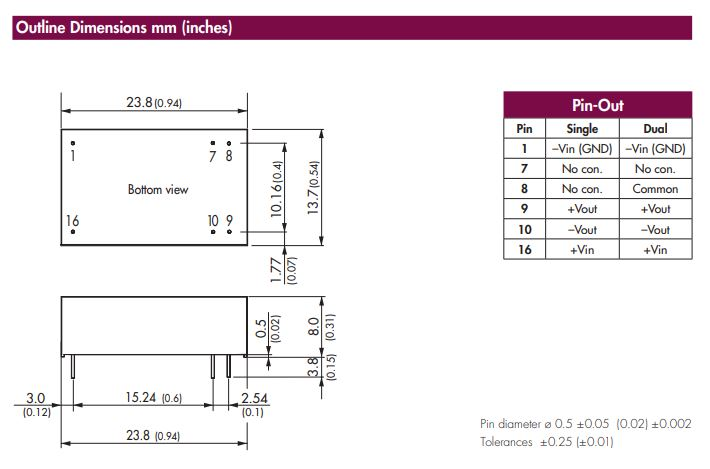
\includegraphics[scale=0.8]{convertidor_5vdc_datasheet}
  \caption{Dimensiones y pinout del convertidor TEL 2-0511 según su hoja de datos.}\label{fig:convertidor_5vdc_datasheet}
\end{figure}

\begin{figure}[!htb]
\minipage{0.4\textwidth}
  \includegraphics[width=\linewidth]{convertidor_5vdc_simbolo}
  \caption{Símbolo creado en Eagle del convertidor TEL 2-0511.}\label{fig:convertidor_5vdc_simbolo}
\endminipage\hfill
\minipage{0.4\textwidth}
  \includegraphics[width=\linewidth]{convertidor_5vdc_huella}
  \caption{Huella creada en Eagle del convertidor TEL 2-0511.}\label{fig:convertidor_5vdc_huella}
\endminipage\hfill
\end{figure}

\begin{figure}[!htb]
\centering
\includegraphics[scale=0.7]{convertidor_15vdc_datasheet}
  \caption{Dimensiones y pinout del convertidor TDR 3-0513SM según su hoja de datos.}\label{fig:convertidor_15vdc_datasheet}
\end{figure}

\begin{figure}[!htb]
\minipage{0.5\textwidth}
  \includegraphics[width=\linewidth]{convertidor_15vdc_simbolo}
  \caption{Símbolo creado en Eagle del convertidor TDR 3-0513SM.}\label{fig:convertidor_15vdc_simbolo}
\endminipage\hfill
\minipage{0.3\textwidth}
  \includegraphics[width=\linewidth]{convertidor_15vdc_huella}
  \caption{Huella creada en Eagle del convertidor TDR 3-0513SM.}\label{fig:convertidor_15vdc_huella}
\endminipage\hfill
\end{figure}

Una vez se dispone de todos los componentes necesarios, se genera con ellos el esquemático de la etapa de potencia del mini TEREFES mostrado en la figura \ref{fig:pcb_potencia_esquematico}. Este diseño dispone únicamente de los componentes necesarios para la etapa de potencia del electroestimulador de la prótesis híbrida. Estos son, entrada de $5Vdc$ desde una batería externa, una fuente de $5Vdc$ y una fuente de $15Vdc$ y $\pm15Vdc$. Los puntos más importantes del esquemático son:

\begin{itemize}
\item[•] \textbf{Conector JP1:} entrada de $5Vdc$ desde la batería mediante este conector de cuatro pines, pues se conecta en serie un interruptor para poder cortar la alimentación y apagar el dispositivo.
\item[•] \textbf{Componentes U1, U2 y U3:} son los convertidores de corriente continua de $5Vdc$ a $5Vdc$, $5Vdc$ a $15Vdc$ y $5Vdc$ a $\pm15Vdc$ respectivamente.
\item[•] \textbf{Conectores JP2, JP3 y JP4:} Son los conectores que portan las salidas de los convertidores, es decir los niveles de tensión de $5Vdc$, $15Vdc$ y $\pm15Vdc$ y sus referencias a masa que necesita la tarjeta de control. Son estos los conectores que se desea alinear con los correspondientes de le placa de control en el montaje con los reversos enfrentados.
\item[•] \textbf{Conector JP5:} Este conector sirve para el control de encendido y apagado del convertidor U3. Si se desea encender el convertidor se ha de conectar el pin RC de U3 a su masa, es decir, -VIN la cual va a su vez conectada a la masa de la batería. Por el contrario, si se desea apagar el convertidor se ha de poner un nivel de tensión de $5Vdc$ en el pin RC. También se desea alinear este conector con su correspondiente punto en la placa de control.
\item[•] Se han añadido varios ``testpoints'' en los que poder medir fácilmente diferentes niveles de tensión, como la salida de los convertidores, una vez la placa esté fabricada y en funcionamiento.
\end{itemize}


\subsubsection{Tarjeta de circuito impreso}
Una vez finalizado el esquemático de la etapa de potencia del mini TEREFES, se genera ahora la distribución o ``layout'' de las huellas de todos sus componentes en la tarjeta de circuito impreso que los contendrá. 
\\
\\
Es un diseño sencillo por lo que dos capas son suficientes: la superior contiene todos los componentes y conexiones mientras que la inferior es el plano de masa de la batería y la conexión del pin RC del convertidor U3 al conector JP5. Además, para que la tarjeta disponga de conexiones a masa y señales robustas, se ha decidido utilizar polígonos en vez de pistas siguiendo el diseño de la tarjeta de potencia del TEREFES.
\\
\\
El punto más importante es la colocación de los conectores JP2, JP3 y JP4. Deben quedar alineados con los puntos correspondientes de la tarjeta de circuito impreso de la etapa de control. Para ello se han de tomar medidas sobre ésta y aplicarlas consecuentemente a los conectores mencionados. Se muestra entonces en la figura \ref{fig:pcb_control_layout} del Anexo I el anverso de la placa de control con las medidas mencionadas. Ahora, para la colocación de los conectores JP2, JP3 y JP4 en la placa de potencia se ha de considerar la imagen especular de los conectores correspondientes de la placa de control según uno de los lados verticales. Esto es lo miso que lo ya explicado en la figura \ref{fig:montaje_alineado}. Se muestra en la figura \ref{fig:pcb_potencia_layout} la distribución de los componentes de la tarjeta de la etapa de control. Sin embargo, se puede ver que las medidas verticales tomadas sobre las placas de potencia y control no coinciden, las de la tarjeta de potencia son $1mm$ más largas. Los conectores de ambas placas están alineados, pero se ha hecho la placa de potencia $1mm$ más larga. Esto es así para que los polígonos que utilizan los conectores JP3 y JP4 los rodeen totalmente y la conexión eléctrica sea robusta.
\\
\\
Se pueden apreciar también en el Anexo II la capa superior, inferior y el modelo de fabricación de la tarjeta de potencia en las figuras \ref{fig:pcb_potencia_top}, \ref{fig:pcb_potencia_bottom} y \ref{fig:pcb_potencia_modelo} respectivamente.\\

\subsection{Validación de objetivos}


\section{Etapa de control}
La etapa de control es mucho más robusta que la de potencia. Sin embargo, existen vías de mejora cuya implementación se explica en este apartado.

\subsection{Revisión del hardware y planteamiento de objetivos de mejora}
Se ha mencionado con anterioridad que la tarjeta de la etapa de potencia tiene un convertidor de corriente continua de $5Vdc$ a $\pm15Vdc$. Este convertidor dispone de una entrada denominada RC o ``Remote Control'' que según su hoja de datos controla el encendido y apagado del mismo. Esto permite que en su salida haya $\pm15Vdc$ o $0Vdc$. En el diseño original de la etapa de potencia del estimulador se hace este tipo de control, lo cual se mantiene tras mejorar el hardware de dicha etapa según el apartado \ref{mejora_hardware_potencia}. Esta funcionalidad permite reducir el consumo del electroestimulador mientras esté encendido pero no utilizándose para aportar asistencia al paciente.
\\
\\
Para llevar a cabo el control remoto del convertidor de $\pm15Vdc$ se ha de manejar el nivel de tensión en su entrada RC. Si se desea apagar el convertidor, esta entrada debe estar a $5Vdc$. Si por el contrario, se desea encenderlo, RC debe estar conectada a la masa del convertidor. Es el microcontrolador ATmega128L de la etapa de control el que efectúa el encendido y apagado. Para ello, se sirve del puerto G1 conectado a RC mediante uno de los dos pines de la conexión 2 de la figura \ref{fig:pcb_control_layout}. Esta conexión es una de las que se ha discutido en la mejora del hardware de la etapa de potencia, pues queda alineada en el montaje de reversos enfrentados con su correspondiente punto en la placa de dicha etapa. Se aprecia la conexión descrita en las figuras \ref{fig:RC_convertidor_control} y \ref{fig:RC_convertidor_potencia}.\\

\begin{figure}[!htb]
\minipage{0.45\textwidth}
  \includegraphics[width=\linewidth]{RC_convertidor_control}
  \caption{Conexión del microcontrolador a un pin montado en la placa de control. Este pin se conecta a su vez con un jumper a la entrada RC del convertidor de $5Vdc$ a $\pm15Vdc$ en la tarjeta de potencia.}\label{fig:RC_convertidor_control}
\endminipage\hfill
\minipage{0.45\textwidth}
  \includegraphics[width=\linewidth]{RC_convertidor_potencia}
  \caption{Conexión para el control remoto del convertidor de $5Vdc$ a $\pm15Vdc$ mediante un cable desde la etapa de control.}\label{fig:RC_convertidor_potencia}
\endminipage\hfill
\end{figure}

Se puede ver en la figura \ref{fig:RC_convertidor_control} cómo un cable rojo une el puerto G1 del microcontrolador con el pin situado entre los leds amarillo y rojo. Esto es un punto débil en la etapa de control ya que esta conexión no es óptima en términos eléctricos ni mecánicos. Esto se explica porque la soldadura puede no ser correcta al formarse un puente con los pines colindantes del microcontrolador o el cable puede presentar problemas. Se plantea entonces una alternativa para sustituir esta conexión por otra implementada de una forma más robusta y fiable sin tener que rediseñar la tarjeta de circuito impreso. Para ello, se tomará ventaja del hecho de que la placa de control también está diseñada para el estimulador TEREFES, el cual tiene dos fuentes de $15Vdc$ y $\pm15Vdc$. Esto permite el uso de una de las pistas de la tarjeta de control que no se ha utilizado ya que se empleaba para una de la fuentes de tensión del TEREFES que no tiene el mini TEREFES.

\subsection{Tareas para la mejora del hardware}
Se puede ver en la figura \ref{fig:pcb_control_layout} del Anexo I, junto a la conexión 2, otras tres conexiones denominadas D1, D2 y D4. Se pueden ver más fácilmente dichas conexiones en la parte inferior izquierda de la imagen representativa de la placa en el Anexo I. En estas conexiones se sitúan tres leds los cuales indican si la estimulación eléctrica está activa, si el convertidor de $5Vdc$ a $\pm15Vdc$ está encendido y si el estimulador está encendido, respectivamente. Sin embargo, D3, es decir la conexión 2, se utiliza para el control remoto del convertidor tal y como ya se ha explicado.
\\
\\
Cuando esta tarjeta de circuito impreso se utilizaba en el TERFES, en la conexión 2 había un led que indicaba el estado del segundo convertidor de $5Vdc$ a $\pm15Vdc$. Sin embargo, en el mini TEREFES no se utiliza la pista que une el alojamiento de dicho led con el puerto E4 del microcontrolador, el cual lo enciende o apaga.
\\
\\
Lo que se propone es prescindir del cable que une el puerto G1 del microcontrolador con el pin que lleva al control remoto del convertidor. A continuación, se desea implementar el control remoto mediante el puerto E4 que está unido con una pista al alojamiento D3 o lo que es lo mismo, la conexión 2 mencionada previamente. En éste se encuentran los pines que se conectan al RC del convertidor y su referencia a masa de la forma explicada en el apartado de mejora del hardware de la etapa de potencia. Se expone con más detalle este procedimiento en la figura \ref{fig:mejora_RC}. En esta figura se aprecia que la unión azul, la de la pista en la tarjeta de circuito impreso, está dividida por dos cuadros naranjas. Éstos representan la huella de la resistencia originalmente une el puerto del microcontrolador con el pin RC. La resistencia era necesaria cuando en esta conexión se alojaba el led que indicaba el estado del segundo convertidor del TEREFES. En el caso del mini TEREFES no es necesario utilizarla por lo que la pista se cierra utilizando una resistencia de $0\Omega$.\\

\begin{figure}[!htb]
\centering
\includegraphics[scale=0.7]{mejora_RC}
  \caption{Representación del control del convertidor desde el microcontrolador. La unión roja es el cable del que se desea prescindir mientras que la unión azul es la pista de la tarjeta de circuito impreso que se va a utilizar. El rectángulo azul representa la conexión 2 de la figura \ref{fig:pcb_control_layout} que contiene los pines que se conectan a la referencia de masa y RC del convertidor que se desea controlar.}\label{fig:mejora_RC}
\end{figure}

Esta tarea de mejora conlleva inevitablemente modificar el firmware del electroestimulador. Esto se debe a que el control remoto del convertidor de $5Vdc$ a $\pm15Vdc$ se hace ahora mediante el puerto E4 y no el G1. Se muestran a continuación las líneas de código que se encargan del control remoto del convertidor mediante el puerto G1:

\begin{lstlisting}[language=C++,breaklines]
case CMD_ON1:	//se desea encender la fuente 
	PORTG &= ~(1<<PORTG1);	//Encender fuente, 0Vdc a RC mediante PG1
	PORTE |= (1<<PORTE3);	//Encender led de estado de fuente
	
case CMD_OFF1:	//se desea apagar la fuente 
	PORTG |= (1<<PORTG1);	//Apagar fuente, 5Vdc a RC mediante PG1
	PORTE &= ~(1<<PORTE3);	//Apagar led de estado de fuente
\end{lstlisting}

Estas líneas se modifican para hacer uso del puerto E4:

\begin{lstlisting}[language=C++,breaklines]
case CMD_ON1:	//se desea encender la fuente 
	PORTE &= ~(1<<PORTE4);	//Encender fuente, 0Vdc a RC mediante PE4
	PORTE |= (1<<PORTE3);	//Encender led de estado de fuente
	
case CMD_OFF1:	//se desea apagar la fuente 
	PORTE |= (1<<PORTE4);	//Apagar fuente, 5Vdc a RC mediante PE4
	PORTE &= ~(1<<PORTE3);	//Apagar led de estado de fuente
\end{lstlisting}

Se puede ver que se hace uso de un ``switch case'' para la interpretación de tareas en el microcontrolador según el comando indicado. Para el caso los comandos son CMD\_ON1 y CMD\_OFF1 para encender y apagar el convertidor, respectivamente. 
\\
\\
Para que el uso del PE4 sea efectivo, se ha de establecer el valor correcto en el registro de direcciones del puerto E del microcontrolador. De este modo, el puerto E4 debe estar configurado como salida por lo que el bit 3 del registro DDRE debe contener un valor de 1 tal y como se indica a continuación:

\begin{lstlisting}[language=C++,breaklines]
DDRE |= ((1<<DDE2) | (1<<DDE3) | (1<<DDE4) | (1<<DDE5) | (1<<DDE6) | (1<<DDE7));
\end{lstlisting}
\subsection{Validación de objetivos}
Según las tareas descritas en el apartado anterior, se ha eliminado el cable que une el puerto G1 del microcontrolador con el pin que conecta al control remoto del convertidor. Además, se ha cerrado la pista de la tarjeta de control con una resistencia de $0\Omega$. De este modo, es ahora el puerto E4 del ATmega128L el que controla el encendido y apagado del convertidor de $\pm15Vdc$ tal y como se deseaba. Se aprecia en la figura \ref{fig:mejora_RC_terminado} la mejora efectuada en el hardware, así como su validación en la figura \ref{fig:mejora_RC_terminado} que muestra la fuente de tensión encendida tras esta mejora.\\

\begin{figure}[!htb]
\minipage{0.45\textwidth}
  \includegraphics[width=\linewidth]{mejora_RC_terminado}
  \caption{Tarjeta de control tras la mejora del hardware para el control remoto del convertidor de $\pm15Vdc$. Se aprecia que ya no hay ningún cable soldado al PG1 así como hay una resistencia de $0\Omega$ en la pista señalada en azul, junto al PE4.}\label{fig:mejora_RC_terminado}
\endminipage\hfill
\minipage{0.45\textwidth}
  \includegraphics[width=\linewidth]{mejora_RC_terminado}\caption{Medición en la salida del convertidor de $\pm15Vdc$. El convertidor se ha encendido mediante el control remoto haciendo uso del PE4 del microcontrolador.}\label{fig:mejora_RC_terminado}
\endminipage\hfill
\end{figure}


\chapter{Optimización del firmware de los electroestimuladores}
En el presente capítulo se procede al estudio y mejora del firmware de los electroestimuladores de la prótesis híbrida. Se desea obtener un firmware optimizado en cuanto velocidad y eficiencia de comunicación con el exterior. Esto se debe a la necesidad de la rapidez por parte de los mismos para modificar parámetros de estimulación durante la realización de los ejercicios de rehabilitación.
\\
\\
Al igual que en el capítulo anterior, se identificarán los objetivos de mejora, en este caso del firmware, para poder plantear así tareas dedicadas a su mejora y optimización.
\\
\\
Por último, se validará el cumplimiento de las tareas mencionadas para culminar en una comparación de las versiones del firmware original y optimizada.

\section{Revisión del firmware y planteamiento de objetivos de mejora}
Tal y como se ha explicado en el capítulo \ref{capitulo_2} el electroestimulador mini TEREFES es capaz de comunicarse con el exterior mediante interrupciones por USART. De este modo, puede recibir comandos como el siguiente:

$$w\;0\;ap\;30\;\textbackslash r$$

lo cual significa escribir en el canal cero una amplitud de pulso positiva de 30$mA$.
\\
\\
Estos comandos se reciben como cadenas de caracteres lo que la instrucción anterior consta de diez, incluyendo espacios y el retorno de carro ($\textbackslash r$) para indicar el final de comando. Además, es necesario considerar que cada carácter tiene un tamaño de 1 byte por lo que el comando expuesto ocupa 10 bytes. Esto es importante debido a que los Registros de Datos del USART o UDR del microntrolador tienen un tamaño de 1 byte. Estos registros son los encargados de almacenar los datos que se reciben (registro de recepción) o transmiten (registro de transmisión) a través del puerto serie. En el caso se utiliza el USART1 por lo que sus registros de datos son UDR1 (los registros de transmisión y recepción comparten a misma dirección de entrada/salida o Input/Output. Cuando se escriben datos en UDR1 se almacenan en el registro de transmisión mientras que si se efectúa una lectura de UDR1 se accede al contenido del registro de recepción.) Se aprecia en la figura \ref{fig:USART_datasheet} la descripción del registro de datos del USART según la hoja de datos del ATmega128L.\\

\begin{figure}[!htb]
\centering
\includegraphics[scale=0.45]{USART_datasheet}
  \caption{Descripción del registro de datos asociado al USART del ATmega128L según su hoja de datos.}\label{fig:USART_datasheet}
\end{figure}

Analizando la la instrucción anterior que sirve de ejemplo, se observa que la forma de transmitir comandos al electroestimulador está implementada a alto nivel, es decir de cara al usuario que los transmite mediante una terminal y una conexión al puerto serie virtual correspondiente, tal y como se explicó en el capítulo \ref{capitulo_2}. El control de los estimuladores eléctricos en la prótesis híbrida requiere que el microcontrolador que sirve de nodo central efectúe la comunicación con estos dispositivos. Esto implica un control a un nivel más bajo, es decir, el usuario no tendrá contacto directo con estos comandos los cuales serán interpretados por el microcontrolador central para efectuar las correspondientes acciones. Incluso los datos solicitados a los estimuladores en cuanto a sus parámetros serán interpretados por la interfaz gráfica para mostrarlos por pantalla de la forma adecuada. 
\\
\\
Se puede ver cómo la implementación de los comandos en alto nivel deja de ser necesaria. Además, ésta presenta la principal desventaja que concierne al tamaño de los paquetes de datos que se transmiten y lo que en última instancia, influye a la velocidad de ajuste de parámetros de estimulación y la eficiencia en la asistencia durante la rehabilitación. Además, si un solo carácter se pierde o altera durante la comunicación, la instrucción completa será erróena.
\\
\\
Por lo tanto, el principal objetivo de mejora del firmware del estimulador es la codificación de instrucciones que recibe el mini TEREFES para que queden a un nivel más bajo y la comunicación sea más eficiente. 


\section{Codificación de instrucciones del estimulador eléctrico}
Para la tarea de codificación de instrucciones ha de considerar como factor limitante el tamaño del Registro de Datos del USART UDR1. Esto implica necesariamente trabajar con paquetes de datos de 1 byte ya que el microcontrolador no puede recibir o envíar más bytes de una vez. Cabe la posibilidad de utilizar 9 bits para datos pero esto no es compatible con todos los dispositivos que se puedan conectar con el estimulador, por lo que se mantiene la configuración original.
\\
\\
Antes de entrar en la codificación de instrucciones, se va a mostrar la totalidad de comandos que puede recibir el estimulador eléctrico. Estas instrucciones se muestran en la tabla \ref{tabla:comandos_originales}

\begin{table}
  \begin{tabular}{| c | c | c |}
      \hline
      \thead{Instrucción} & \thead{Valor numérico} & \thead{Descripción} \\
      \hline
      w <valor 1> ap <valor 2> &  \makecell{valor 1: [0,3]\\valor 2: [0,50]$mA$} & \makecell{Configuración de la amplitud de pulso positivo\\ recogida en el valor 2 para el canal\\ indicado por el valor 1.}  \\
      \hline
      w <valor 1> an <valor 2> &  \makecell{valor 1: [0,3]\\valor 2: [0,50]$mA$} & \makecell{Configuración de amplitud de pulso negativo\\ recogida en el valor 2 para el canal\\ indicado por el valor 1.}  \\
      \hline
      w <valor 1> re <valor 2> &  \makecell{valor 1: [0,3]\\valor 2: [0,3]} & \makecell{Configuración del número de repeticiones \\de pulso indicadas en valor 2\\ para el canal recogido en valor 1.} \\
      \hline
      w <valor 1> tp <valor 2> &  \makecell{valor 1: [0,3]\\valor 2: [250,500]$\mu s$} & \makecell{Configuración del ancho de pulso positivo\\ recogido en el valor 2 para el canal\\ indicado por el valor 1.}\\
      \hline
      w <valor 1> tn <valor 2> &  \makecell{valor 1: [0,3]\\valor 2: [250,500]$\mu s$} & \makecell{Configuración del ancho de pulso negativo\\ recogido en el valor 2 para el canal\\ indicado por el valor 1.}\\      
      \hline      
      w <valor 1> in <valor 2> &  \makecell{valor 1: [0,3]\\valor 2: [0,1]} & \makecell{Configuración de la inversión \\del canal indicado en valor 1}\\      
      \hline       
      e fl <valor> & \makecell{valor: [0,3]} & \makecell{Configuración del número de canales.}\\      
      \hline    
      e lc <valor 1> <valor 2> &  \makecell{valor 1: [0,3]\\valor 2: [0,3]} & \makecell{Configuración de la lista de turnos \\de los canales. El valor 1 indica el\\ canal y el valor 2 su turno.}\\      
      \hline    
      e tg <valor> &  \makecell{valor: [20,100]Hz} & \makecell{Configuración de la frecuencia inter pulso.}\\      
      \hline  
      e ti <valor> &  \makecell{valor: [20,100]Hz} & \makecell{Configuración de la frecuencia intra pulso.}\\      
      \hline  
      e rm <valor> &  \makecell{valor: [0,3]} & \makecell{Configuración de la repetición máxima.}\\      
      \hline  
      e md <valor> &  \makecell{valor: [1,6]} & \makecell{Configuración del modo de funcionamiento.}\\      
      \hline  
      fap/fan/ftp/ftn/fre/fin <valores> &  \makecell{valores de ap, an,\\ tp, tn, re, in} & \makecell{Configuración rápida de los parámetros ap, an,\\ tp, tn, re e in. Los valores de dichos parámetros\\ se indican en el orden especificado por \\la lista de canales.}\\      
      \hline 
      r0/r1/r2/r3 &  - & \makecell{Lectura de parámetros de los canales 0, 1,\\ 2 o 3. El estimulador devuelve por USART \\los parámetros ap, an, re, tp, tn,\\ re e in del canal especificado.}\\   
      \hline
      l tg/l ti/l md/l fl/l rm/l lc &  - & \makecell{Lectura de los parámetros tg, ti,\\ md, fl, rm y lc respectivamente.}\\         
      \hline      
      on1/off1 &  - & \makecell{Comandos para encender o apagar el\\ convertidor de $5Vdc$ a \\$\pm15Vdc$, respectivamente.}\\         
      \hline          
      s/p &  - & \makecell{Comandos para iniciar o detener\\la estimulación, respectivamente.}\\ 
      \hline          
      g &  - & \makecell{Instrucción para guardar los\\ parámetros de estimulación en la\\ EEPROM del microcontrolador.}\\              
      \hline                                           
  \end{tabular}\caption{Instrucciones originales del mini TEREFES.}\label{tabla:comandos_originales}
\end{table}


\section{Validación de la configuración óptima del firmware}

\chapter{Selección y programación del microcontrolador de la prótesis híbrida}

En el presente capítulo se va a plantear el conjunto de requisitos para la selección del microcontrolador que gobernará el funcionamiento de la prótesis híbrida.
\\
\\
Una vez planteadas las opciones disponibles para dicha selección, se analizarán todas ellas y se escogerá la más adecuada para la prótesis híbrida.
\\
\\
A continuación, se procederá a la implementación de los protocolos de comunicación entre los componentes de la prótesis así como a la programación del microcontrolador seleccionado.

\section{Selección del microcontrolador de la prótesis híbrida}
En primer lugar, se ha de llevar a cabo un análisis de los requerimientos de la prótesis híbrida los cuales van a imponer unos criterios de selección del microcontrolador que la gobierne. A continuación, se deben valorar los microcontroladores disponibles en el mercado que se ajusten a los requisitos planteados por la prótesis para proceder a la selección del más adecuado.

\subsection{Requisitos del microcontrolador}
El principal requisito para la selección del microcontrolador se centra en los protocolos de comunicación entre este dispositivo y el resto de componentes de la prótesis híbrida.
\\
\\
Para la comunicación con el exoesqueleto solamente está disponible la comunicación inalámbrica mediante WiFi, por lo que este protocolo debe estar integrado en el microcontrolador.
\\
\\
Por otra parte, se desea explorar la comunicación inalámbrica y cableada con los estimuladores eléctricos. Para la primera opción se pretende utilizar Bluetooth o Bluetooth de baja energía (BLE). En el caso de la segunda opción, lo más adecuado es utilizar UART ya que el mini TEREFES solamente dispone de un conector para la comunicación mediante dicho protocolo. Se podría utilizar I2C o SPI puesto que el ATmega128L embarcado en el estimulador los soporta. Sin embargo, habría que modificar el diseño de la tarjeta de circuito impreso de la etapa de control para añadir el conector correspondiente. Esta tarea no se considera para el proyecto en el que está involucrado el presente trabajo por lo que I2C y SPI quedan descartados.
\\
\\
En el caso de la comunicación con la interfaz gráfica de usuario, se apunta hacia un método inalámbrico siendo el más sencillo y adecuado Bluetooth o BLE.
\\
\\
En cuanto a la capacidad computacional del microcontrolador, es preciso tener en cuenta que este dispositivo actúa como nodo central de la prótesis completa, por lo que la característica mencionada ha de ser uno de los puntos fuertes de este dispositivo. Es más, este dispositivo debe efectuar las siguientes tareas:

\begin{itemize}
\item[•] Comunicación con el exoesqueleto y estimuladores eléctricos durante el ejercicio de rehabilitación. Esta tarea conlleva la recepción y procesamiento de datos provenientes de dichos componentes además llevar a cabo el control de su comportamiento.
\item[•] Recepción y procesamiento de datos provenientes de los sensores utilizados en la prótesis.
\item[•] Recepción y procesamiento de datos provenientes de la interfaz gráfica de usuario así como llevar a cabo una comunicación bidireccional con la misma.
\end{itemize}

Estas tareas deben realizarse dentro de un intervalo temporal impuesto por el ciclo de marcha el cual tiene una duración media para adultos de 0.98 a 1.07s\cite{duracion_ciclo_marcha}. Sin embargo, es preciso considerar que el ciclo de marcha se divide en fases y subfases cada una de ellas pudiendo ser de mucha menor duración que la del ciclo completo. La prótesis híbrida debe ser capaz de actuar dentro de estas fases y subfases llegando a tener una duración del $10\%$ del ciclo de marcha\cite{duracion_fases_ciclo_marcha}, lo que significa límites temporales de unos $100ms$. Dado el número de tareas que debe realizar el microcontrolador dentro de los límites temporales expuestos así como el hecho de que debe actuar de nodo central de la prótesis híbrida, se descartan los microcontroladores de 8 bits ya que pueden resultar insuficientes.


\subsection{Selección del microcontrolador}

Para la selección del microcontrolador más adecuado se tiene en consideración un factor fundamental para el proyecto: la velocidad de integración del mismo en la prótesis híbrida. Es por esto por lo que se prefiere adquirir una placa de desarrollo en vez de el microcontrolador y crear para el mismo una tarjeta de circuito impreso que lo contenga así como el resto de componentes necesarios.
\\
\\
Dados los requisitos expuestos previamente, las placas de desarrollo que más se ajustan a los mismos son las creadas por Espressif\cite{espressif}. Estas placas contienen las series de módulos ESP32, ESP32-S2 y ESP8266 que a su vez integran las series de sistemas en chip con los mismos nombres. Estas series ofrecen numerosos microcontroladores de 32 bits principalmente orientados a las comunicaciones mediante WiFi, Bluetooth y BLE, control de periféricos y modos de bajo consumo para el ahorro de energía. Se muestra en la imagen \ref{fig:placa_modulo_soc} la configuración descrita.\\

\begin{figure}[!htb]
\centering
\includegraphics[scale=0.4]{placa_modulo_soc}
  \caption{De izquierda a derecha: sistema en chip, módulo de la serie ESP32 y placa de desarrollo de la serie ESP32.}\label{fig:placa_modulo_soc}
\end{figure}

La serie de kits de desarrollo que se ajusta a los requisitos de selección es la ESP32 ya que soporta WiFi, Bluetooth y BLE. Dentro de esta serie, es necesario descartar todas aquellas placas orientadas a procesamiento digital de señales, procesamiento de audio y vídeo, reconocimiento de voz y demás características que no son necesarias para la prótesis híbrida. Se desea además una placa de desarrollo de tamaño reducido para su fácil integración en la estructura de la prótesis.
\\
\\
Dentro de la serie mencionada, quedan entonces dos opciones: el ESP32-DevKitC y el ESP32-PICO-KIT. La segunda de estas dos placas es la más pequeña con un tamaño de 52 x 20.3 mm\cite{picokit}. Sin embargo, no tiene ningún tipo de antena integrada lo cual requiere un análisis de la más adecuada, su adquisición, instalación y comprobación de su correcto funcionamiento. Se descarta esta placa de desarrollo ya que la ESP32-DevKitC es la que más se ajusta a los requisitos de selección, tiene antena integrada en la tarjeta de circuito impreso y su tamaño no es mucho mayor que el de la ESP32-PICO-KIT con unas medidas de 54.4 x 27.9 mm\cite{devkitc}.
\\
\\
Una vez seleccionada la placa de desarrollo ESP32-DevKitC, se ha de determinar cuál de sus posibles módulos es el más adecuado para la prótesis híbrida. Para ello se lleva a cabo un análisis de los módulos disponibles en la tablas \ref{tabla:modulos_esp32_1} y \ref{tabla:modulos_esp32_2}.
\\
\\
Analizando estas tablas, se aprecia en primer lugar que hay tres módulos que no tienen la antena integrada sino un conector para que el usuario acople una. Al igual que el caso del ESP32-PICO-KIT, se descartan estos módulos por el motivo ya explicado. Además, no es necesaria una transmisión de datos inalámbrica a larga distancia o con obstáculos en el camino ya que los componentes de la prótesis estarán cercanos entre sí. Por lo tanto, la antena integrada es la mejor opción.
\\
\\
Otro punto en el que difieren los módulos resultantes es su CPU. El ESP32-WROOM-32E y el ESP32-WROVER-E tienen una CPU de dos núcleos mientras que la del ESP32-SOLO-1 tiene uno. Esto implica que la opción de dos núcleos consume más energía. De hecho, en la tabla \ref{tabla:modulos_esp32_1} se aprecia un consumo máximo de casi el doble por parte de la CPU de dos núcleos en comparación con la de uno. Sin embargo, este consumo es el que se produce a la velocidad de reloj máxima: 240MHz para la CPU de dos núcleos y 160MHz para la de uno. Cuando esta velocidad se reduce a 80MHZ, lo cual es lo más probable para la aplicación del presente trabajo, los consumos de ambas CPUs son prácticamente iguales\cite{esp32_consumo_cpu}. Por tanto, se elige la CPU de dos núcleos ya que aporta más versatilidad y potencia de procesamiento con un consumo similar a la CPU de un núcleo para la configuración de velocidad de reloj ya explicada.
\\
\\
Solamente queda elegir entre los módulos ESP32-WROOM32-E y ESP32-WROVER-E. Su principal diferencia es la RAM: el primero tiene 520KB on chip mientras que el segundo tiene además 8MB de Pseudo SRAM o PSRAM. Los requisitos de selección del microcontrolador no especifican un manejo ni almacenamiento de datos considerable por lo que no se requiere una SRAM excesivamente grande. En consecuencia, se descarta el módulo ESP32-WROVER-E puesto que no es necesario tener la memoria RAM sobredimensionada.
\\
\\
Se muestra en la imagen \ref{fig:seleccion_placa} la placa de desarrollo seleccionada: ESP32-DevKitC-32E.

\begin{figure}[!htb]
\centering
\includegraphics[scale=0.5]{seleccion_placa}
  \caption{Placa de desarrollo Espressif ESP32-DevKitC-32E.}\label{fig:seleccion_placa}
\end{figure}

\begin{landscape}

\begin{table}[]
\centering
\begin{tabular}{|c|c|c|c|c|c|c|}
\hline
\begin{tabular}[c]{@{}c@{}}Placa \\ de desarrollo\end{tabular} & Módulo                                & Antena                            & CPU                                                                                                         & \begin{tabular}[c]{@{}c@{}}Consumo \\ máximo CPU\cite{esp32_consumo_cpu}\end{tabular}                       & FLASH                & RAM                                                                      \\ \hline
\multirow{6}{*}{ESP32-DevKitC}                                 & ESP32-SOLO-1                          & \multirow{3}{*}{Integrada}        & \begin{tabular}[c]{@{}c@{}}ESP32-S0WD \\ Single Core\\ 32 bits\\ 160MHz max.\end{tabular}                   & \begin{tabular}[c]{@{}c@{}}34mA a 3,3V\\ 112mW aprox.\end{tabular}                  & \multirow{3}{*}{4MB} & \multirow{2}{*}{\begin{tabular}[c]{@{}c@{}}520KB\\ on chip\end{tabular}} \\ \cline{2-2} \cline{4-5}
                                                               & ESP32-WROOM-32E                       &                                   & \multirow{2}{*}{\begin{tabular}[c]{@{}c@{}}ESP32-D0WD-V3 \\ Dual Core\\ 32 bits\\ 240MHz max.\end{tabular}} & \multirow{2}{*}{\begin{tabular}[c]{@{}c@{}}68mA a 3,3V\\ 225mW aprox.\end{tabular}} &                      &                                                                          \\ \cline{2-2} \cline{7-7} 
                                                               & ESP32-WROVER-E                        &                                   &                                                                                                             &                                                                                     &                      & \begin{tabular}[c]{@{}c@{}}520KB\\ on chip\\ 8MB\\ PSRAM\end{tabular}    \\ \cline{2-7} 
                                                               & \multicolumn{1}{l|}{ESP32-WROOM-32U}  & \multicolumn{1}{l|}{No integrada} & -                                                                                                           & -                                                                                   & -                    & -                                                                        \\ \cline{2-7} 
                                                               & \multicolumn{1}{l|}{ESP32-WROOM-32UE} & \multicolumn{1}{l|}{No integrada} & -                                                                                                           & -                                                                                   & -                    & -                                                                        \\ \cline{2-7} 
                                                               & \multicolumn{1}{l|}{ESP32-WROVER-IE}  & \multicolumn{1}{l|}{No integrada} & -                                                                                                           & -                                                                                   & -                    & -                                                                        \\ \hline
\end{tabular}
\caption{Comparación de módulos de la serie ESP32\cite{modulos_esp32}.}
\label{tabla:modulos_esp32_1}
\end{table}

\begin{table}[]
\centering
\begin{tabular}{|c|c|c|c|c|c|c|c|}
\hline
\begin{tabular}[c]{@{}c@{}}Placa \\ de desarrollo\end{tabular} & Módulo                                & SPI                 & I2C                 & UART                & Bluetooth                                                                 & WiFi                                                                                        & \begin{tabular}[c]{@{}c@{}}Precio \\ unitario\end{tabular} \\ \hline
\multirow{6}{*}{ESP32-DevKitC}                                 & ESP32-SOLO-1                          & \multirow{3}{*}{x2} & \multirow{3}{*}{x2} & \multirow{3}{*}{x3} & \multirow{3}{*}{\begin{tabular}[c]{@{}c@{}}Bluetooth \\ BLE\end{tabular}} & \multirow{3}{*}{\begin{tabular}[c]{@{}c@{}}IEEE \\ 802.11b/g/n\\ 150Mbps max.\end{tabular}} & \multirow{3}{*}{8€}                                        \\ \cline{2-2}
                                                               & ESP32-WROOM-32E                       &                     &                     &                     &                                                                           &                                                                                             &                                                            \\ \cline{2-2}
                                                               & ESP32-WROVER-E                        &                     &                     &                     &                                                                           &                                                                                             &                                                            \\ \cline{2-8} 
                                                               & \multicolumn{1}{l|}{ESP32-WROOM-32U}  & -                   & -                   & -                   & -                                                                         & -                                                                                           & -                                                          \\ \cline{2-8} 
                                                               & \multicolumn{1}{l|}{ESP32-WROOM-32UE} & -                   & -                   & -                   & -                                                                         & -                                                                                           & -                                                          \\ \cline{2-8} 
                                                               & \multicolumn{1}{l|}{ESP32-WROVER-IE}  & -                   & -                   & -                   & -                                                                         & -                                                                                           & -                                                          \\ \hline
\end{tabular}
\caption{Comparación de módulos de la serie ESP32\cite{modulos_esp32}.}
\label{tabla:modulos_esp32_2}
\end{table}

\end{landscape}



\section{Implementación de los protocolos de comunicación}
Una vez seleccionada la placa de desarrollo ESP32-DevKitC-32E como nodo central de la prótesis, se han de determinar los protocolos de comunicación entre este dispositivo y el resto de los componentes de la misma. Se va a proceder en primer lugar al análisis de los protocolos disponibles para cada componente para continuar con su comparación y finalmente seleccionar los más óptimos.

\subsection{Protocolo con el exoesqueleto}
\subsection{Protocolo con la interfaz}
\subsection{Protocolo con los estimuladores eléctricos}

Se revisa la configuración establecida en el USART1. En primer lugar se aprecia que el Registro C de Configuración y Estado del USART1 contiene el siguiente valor:\\

\begin{lstlisting}[language=C++,breaklines]
UCSR1C = 0x86;
\end{lstlisting}

Esta configuración, según la hoja de datos del microcontrolador, establece los siguientes ajustes en la comunicación serial por USART:

\begin{itemize}
\item[•] Modo de operación asíncrono.
\item[•] Modo de paridad deshabilitado.
\item[•] Un bit de parada.
\item[•] Ocho bits para datos.
\end{itemize}
 
El modo de operación es en efecto asíncrono, lo que quiere decir que los dispositivos conectados al estimulador por puerto serie no se comunican mediante una línea de datos y un reloj compartido. En cambio, como ya se ha visto anteriormente, existe una línea de transmisión y otra de recepción de datos. Por tanto, los dispositivos a ambos extremos de estas líneas deben conocer las características de la comunicación serial. Esto es así porque el estimulador originalmente se comunica de forma inalámbrica lo que imposibilita compartir una línea de reloj con el dispositivo al que se conecta. En cuanto al tamaño de los datos, se utiliza 8 bits por cuestiones de compatibilidad con los dispositivos conectados al microcontrolador.
\\
\\
Por otra parte, observando el valor del registro A de control y estado del USART1 se aprecia que está configurado de la siguiente manera: 

\begin{lstlisting}[language=C++,breaklines]
UCSR1A = 0X02;
\end{lstlisting}

En esta configuración se tiene el segundo bit de dicho registro a un valor de 1 lo que implica la activación de la funcionalidad de doble velocidad para comunicaciones asíncronas. Se muestra en la figura \ref{fig:U2X_datasheet} dicha configuración según la hoja de datos del ATmega128L.\\

\begin{figure}[!htb]
\centering
\includegraphics[scale=0.45]{U2X_datasheet}
  \caption{Descripción del modo de doble velocidad en comunicaciones asíncronas para el ATmega128L según su hoja de datos.}\label{fig:U2X_datasheet}
\end{figure}

Por otro lado, se tienen los registros de configuración de tasa de baudios UBRR1H y UBRR1L en los cuales que se carga el valor contenido en $ubrr$ según la siguiente configuración efectuada en la función de inicialización del USART1:\\

\begin{lstlisting}[language=C++,breaklines]
UBRR1H = (unsigned char)(ubrr>>8);
UBRR1L = (unsigned char)ubrr;
\end{lstlisting}

A partir de ahora se hablará de la velocidad de comunicación en bits por segundo por cuestiones de homogeneidad en la terminología. Se ha tomado esta decisión ya que bits por segundo y baudios no so lo mismo aunque se usen indistintamente de forma extendida.
\\
\\
Teniendo en cuenta el modo de doble velocidad explicado previamente, la frecuencia de reloj del microcontrolador de $8MHz$, y que el valor de $ubrr$ observado en el firmware es de 8, la figura \ref{fig:UBRR_datasheet} obtenida de la hoja de datos muestra que se tiene una velocidad de comunicación USART asíncrona de 115200 bps.\\

\begin{figure}[!htb]
\centering
\includegraphics[scale=0.4]{UBRR_datasheet}
  \caption{Valores del registro de tasa de baudios según la velocidad de reloj y la modalidad de doble velocidad. Se indican en rojo los valores observados en el firmware original del mini TEREFES.}\label{fig:UBRR_datasheet}
\end{figure}

Una vez vista la configuración del USART1 del que se sirve el microcontrolador para comunicarse, se concluye que los factores que se pueden modificar para optimizar la comunicación son su velocidad en bits por segundo, los bits de parada y la paridad de bits. Trabajando con el estimulador se ha observado que una velocidad de 115200bps puede ser demasiado elevada en una aplicación como la que concierne al electroestimulador ya que no se requiere la transmisión de grandes cantidades de datos. Además, ciertas velocidades conllevan probabilidades de errores más elevadas tal y como indica la hoja de datos del ATmega128L en la figura \ref{fig:UBRR_datasheet}. Esto afecta a la integridad de los mensajes y por tanto a la efectividad del estimulador en su asistencia.

Se ha intentado establecer comunicación con el módulo de comunicación inalámbrica del dispositivo desde un ordenador mediante un puerto serie virtual y Bluetooth. Para ello se ha escrito un script en Python el cual se encarga de transmitir comandos al mini TEREFES de la siguiente forma:


\begin{lstlisting}[language=C++,breaklines]
import pyserial

puerto_serie = serial.Serial(
	port = 'COM3',
	baudrate = 115200,
	parity = serial.PARITY_NONE,
	stopbits = serial.STOPBITS_ONE,
	bytesize = serial.EIGHBITS,
	timeout = 2
)

comando = "w 0 ap 30\r"

if puerto_serie.is_open:
	for c in comando:
		puerto_serie.write(c.encode())
		
	if puerto_serie.inWaiting() > 0:
		print(puerto_serie.read().decode())	
\end{lstlisting}

Con este script se establece comunicación con el electroestimulador mediante un puerto serie virtual $COM3$. Entonces, envía a éste el comando ``w 0 ap 30\textbackslash r'' visto con anterioridad y a continuación se recibe por el mismo puerto serie la respuesta del mini TEREFES, pues para esta prueba se ha configurado el firmware para que devuelva los mensajes que recibe. El resultado es la devolución de mensajes incompletos o incoherentes por parte del estimulador indicando una velocidad de comunicación inadecuada. Para corroborar esto, se modifica dicha velocidad para que resulte en 19200 bps, un valor de 51 en el registro UBRR según la figura \ref{fig:UBRR_datasheet} y se observa que los mensajes llegan adecuadamente. 

\subsubsection{USART mediante cable}
Para establecer este tipo de comunicación solamente son necesarios tres cables para formar las líneas de transmisión y recepción de datos y unir las masas de los dispositivos conectados. En la imagen representativa de la placa de control mostrada en el Anexo 1, el conector JP5 es el encargado de la comunicación. Para ello se sirve de cuatro alojamientos en los que alojar cables o el módulo Bluetooth ya visto y que se tratará más adelante. De este modo, se utilizan los alojamientos 2, 3 y 4 del conector JP5 que son la referencia a masa, la línea de transmisión del estimulador y la de recepción, respectivamente.

\subsubsection{USART mediante Bluetooth y BLE}
Para establecer comunicación inalámbrica con el estimulador hay que alojar el módulo Bluetooth en el conector JP5 de la placa de control. Una vez hecho esto, es posible conectarse a dicho módulo desde cualquier dispositivo con Bluetooth y capacidad de comunicación serial. Esto se puede conseguir con un ordenador con Bluetooth y una terminal de puerto serie tal y como se indicó en el capítulo \ref{capitulo_2}.
\\
\\
Para el ajuste de velocidad de comunicación, hay que llevar a cabo lo descrito en el apartado anterior dedicado a la comunicación cableada, esto es, ajustar la velocidad del USART en el mcicrocontrolador.
\\
\\
El siguiente paso es ajustar la velocidad de comunicación en el módulo Bluetooth, para lo cual es útil la documentación ofrecida en la página web del producto. Las herramientas necesarias para esta tarea son el propio módulo Bluetooth Sparkfun Silver Smirf y un Arduino Uno.
\\
\\
En primer lugar se ha de conectar el módulo Bluetooth al Arduino de la manera indicada en la figura \ref{fig:configuracion_modulos_BT}. En cuanto al programa para la configuración del módulo, se utiliza el sugerido por Sparkfun y el cual se muestra a continuación:


\begin{lstlisting}[language=C++,breaklines]
/*
  Example Bluetooth Serial Passthrough Sketch
 by: Jim Lindblom
 SparkFun Electronics
 date: February 26, 2013
 license: Public domain

 This example sketch converts an RN-42 bluetooth module to
 communicate at 9600 bps (from 115200), and passes any serial
 data between Serial Monitor and bluetooth module.
 */
#include <SoftwareSerial.h>  

int bluetoothTx = 2;  // TX-O pin of bluetooth mate, Arduino D2
int bluetoothRx = 3;  // RX-I pin of bluetooth mate, Arduino D3

SoftwareSerial bluetooth(bluetoothTx, bluetoothRx);

void setup()
{
  Serial.begin(9600);  // Begin the serial monitor at 9600bps

  bluetooth.begin(115200);  // The Bluetooth Mate defaults to 115200bps
  bluetooth.print("$");  // Print three times individually
  bluetooth.print("$");
  bluetooth.print("$");  // Enter command mode
  delay(100);  // Short delay, wait for the Mate to send back CMD
  bluetooth.println("U,9600,N");  // Temporarily Change the baudrate to 9600, no parity
  // 115200 can be too fast at times for NewSoftSerial to relay the data reliably
  bluetooth.begin(9600);  // Start bluetooth serial at 9600
}

void loop()
{
  if(bluetooth.available())  // If the bluetooth sent any characters
  {
    // Send any characters the bluetooth prints to the serial monitor
    Serial.print((char)bluetooth.read());  
  }
  if(Serial.available())  // If stuff was typed in the serial monitor
  {
    // Send any characters the Serial monitor prints to the bluetooth
    bluetooth.print((char)Serial.read());
  }
  // and loop forever and ever!
}
\end{lstlisting}

Este programa establece comunicación con el módulo Bluetooth mediante las conexiones en los pines 2 y 3 del Arduino. Lo hace a una velocidad de 9600bps, considerando que la que trae por defecto el módulo es de 115200bps. Una vez cargado, se abre la terminal serie de Arduino y utilizando los comandos de configuración del módulo adecuados, se ajusta la velocidad a la que se va a comunicar. Estos comandos se encuentran también en la web del producto y los necesarios para la tarea que se está tratando son:

\begin{itemize}
\item[•] \$\$\$: Entrada al modo de configuración. Antes de modificar los parámetros del módulo Bluetooth, es necesario ponerlo en el estado de configuración. 
\item[•] SU,<valor>: Este comando permite modificar la velocidad de comunicación del dispositivo en bits por segundo. Los posibles valores son 1200, 2400, 4800, 9600, 19.2, 28.8, 38.4, 57.6, 115K, 230K, 460K, or 921K. Solamente es necesario especificar los dos primeros dígitos por lo que si se desea una velocidad de 115200bps se ha de introducir ``SU,11''.
\item[•] ---: Salir del modo de configuración. Tras introducir este comando el módulo volverá a su funcionamiento normal.
\end{itemize}

\begin{figure}[!htb]
\centering
\includegraphics[scale=0.6]{configuracion_modulos_BT}
  \caption{Conexión del módulo Bluetooth al Arduino para su configuración. La línea de transmisión de datos del módulo se conecta a la de recepción del Arduino, es decir el pin 2. La línea de recepción de datos del módulo Bluetooth se conecta a la de transmisión del Arduino, el pin 3.}\label{fig:configuracion_modulos_BT}
\end{figure}

Al igual que el caso de la comunicación cableada, el dispositivo que se conecta al microcontrolador, en este caso mediante el módulo Bluetooth, debe tener la misma velocidad de comunicación serial que estos dos dispositivos.


\subsubsection{Pruebas de velocidad y selección del protocolo}
pruebas cable vs BT de respuesta fisica y devolver datos con parametros baud rate y codificacion o no

PARAMETROS USART1
Los parámetros del USART1 que se van a modificar son los siguientes:

\begin{itemize}
\item[•] Velocidad de comunicación en bits por segundo.
\item[•] Bits de parada.
\item[•] Paridad de bits.
\end{itemize}

Para modificar la velocidad de comunicación solamente es preciso guardar en los registros UBRRH1 y UBRRL1, los cuales forman el UBRR, los valores correspondientes para cada velocidad, según indica la hoja de datos del microcontrolador. Hay que tener en cuenta que la velocidad del reloj del sistema es de $8MHz$ y que el modo de doble velocidad (U2X) está activado. Esto implica, según la figura \ref{fig:UBRR_datasheet} que las posibles velocidades de comunicación por USART y sus respectivos valores de los registros mencionados son los mostradas en la tabla \ref{tabla:velocidades_USART}.\\

\begin{table}
\centering
\begin{tabular}{| p{20mm} | p{30 mm} |}
\hline
\textbf{UBRR} & \textbf{Velocidad (bps)} \\ \hline
416 & 2400\\ \hline
207 & 4800\\ \hline
103 & 9600\\ \hline
68 & 14400\\ \hline
51 & 19200\\ \hline
34 & 28800\\ \hline
25 & 38400\\ \hline
16 & 57600\\ \hline
12 & 76800\\ \hline
8 & 115200\\ \hline
3 & 230400\\ \hline
3 & 250000\\ \hline
1 & 500000\\ \hline
0 & 1000000\\ \hline
\end{tabular}\caption{Valores del registro de tasa de baudios del USART del ATmega128L para un reloj de $8MHz$ y modo de doble velocidad activado (U2X =1) en USART asíncrono.}\label{tabla:velocidades_USART}
\end{table}

Para modificar los bits de parada y la paridad de bits se utiliza el Registro C de Control y Estado tal y como se muestra en la figura \ref{fig:UCSRNC_datasheet}. Los bits 5 y 4 de este registro ofrecen la posibilidad dedeshabilitar la paridad de bits o utilizar un bit de paridad par o impar. El bit 3 del registro de configuración permite configurar uno o dos bits de parada.\\

\begin{figure}[!htb]
\centering
\includegraphics[scale=0.6]{UCSRNC_datasheet}
  \caption{Configuración de la paridad de bits y los bits de parada en el Registro C de Control y Estado del USART.}\label{fig:UCSRNC_datasheet}
\end{figure}


\section{Programación del microcontrolador}
\subsection{Interfaz gráfica}
\subsection{Exoesqueleto robótico}
\subsection{Estimuladores eléctricos}

\chapter{Desarrollo de una interfaz gráfica de usuario}\label{capitulo_4}
Uno de los objetivos principales del presente trabajo es el desarrollo de una interfaz gráfica de usuario para el control centralizado de la prótesis híbrida planteada en el capítulo \ref{capitulo_1}. Con dicha interfaz se pretende manejar el exoesqueleto, hasta cuatro electroestimuladores así como el conjunto de sensores necesarios.
\\
\\
Este control se efectúa de forma inalámbrica: en primer lugar, la interfaz gráfica establece comunicación con el módulo Bluetooth Sparkfun Silver mencionado en el capítulo \ref{capitulo_2}. A continuación, éste sirve como intermediario para la comunicación entre la interfaz gráfica y la prótesis híbrida, la cual se lleva a cabo mediante los protocolos de comunicación descritos en el capítulo \ref{capitulo_3}.
\\
\\
En el presente capítulo se va a exponer cómo se ha desarrollado la interfaz además de sus características, funcionalidades, capacidades y limitaciones.

\section{Entorno de desarrollo y herramientas}
El entorno de desarrollo elegido para esta aplicación es Visual Studio Code y el lenguaje de programación Python3. El autor del presente trabajo ha elegido dicho entorno de desarrollo porque además de ser gratuito, otorga una gran facilidad a la hora de integrar paquetes y bibliotecas. Además,  presenta una interfaz clara y fácil de utilizar incluso en el desarrollo de proyectos de cierta envergadura. En cuanto al lenguaje de programación, el autor ha seleccionado Python por su flexibilidad, sencillez y la gran cantidad de librerías disponibles para la integración de diferentes herramientas y funcionalidades. Es más, se detallan a continuación todas las necesarias para el desarrollo de esta interfaz:
\begin{itemize}
\item[•] \textbf{tkinter, ttk:} se trata del conjunto de herramientas para el desarrollo de interfaces gráficas que permite crear ventanas que recogen el conjunto de widgets (botones, entradas de texto, listas desplegables etc.) y demás elementos gráficos que dan forma a una interfaz gráfica de usuario.
\item[•] \textbf{pyserial:} es la librería que permite manejar herramientas de comunicación por puerto serie que en este caso se utilizan para la comunicación entre la interfaz y el módulo Bluetooth mencionado en el capítulo \ref{capitulo_2}.
\item[•] \textbf{threading:} la interfaz que se pretende elaborar debe realizar un número considerable de tareas no solamente en paralelo sino en tiempo real. Esto implica la necesidad de tener la capacidad de crear hilos de procesamiento para cumplir con la ejecución de todas las tareas estipuladas.
\item[•] \textbf{matplotlib:} para la creación de gráficos en los que mostrar datos relevantes durante la sesión de rehabilitación. Por ejemplo, es importante conocer las medidas de ángulos recibidas por los electrogoniómetros y/o exoesqueleto y que permiten apreciar, en una de sus diferentes formas, las etapas del ciclo de marcha.
\item[•] \textbf{numpy:} para el tratamiento rápido y eficaz de conjuntos extensos de datos.
\end{itemize}



\section{Integración de estimuladores}
Una de las capacidades de la mencionada interfaz de usuario es el control de hasta cuatro electroestimuladores. Se detalla a continuación el conjunto de funcionalidades que se desean implementar en la interfaz en cuanto al control de estos dispositivos se refiere:

\begin{itemize}
\item[•] Seleccionar el número de dispositivos que se van a utilizar.
\item[•] Establecer el valor de todos los parámetros de cada estimulador de manera correcta. Esto implica que estén dentro del rango de valores de corriente, ancho de pulso y frecuencia explicados en el capitulo anterior así como contrarrestar la conversión interna que el estimulador efectúa sobre dichos parámetros.
\item[•] Leer el valor de los parámetros ya configurados en el dispositivo.
\item[•] Guardar los valores de los parámetros configurados en la EEPROM del estimulador.
\item[•] Guardar y cargar todos los parámetros del mini TEREFES en un archivo de texto externo.
\item[•] Configurar el modo de operación de cada estimulador así como controlar el estado de su fuente de corriente (apagada o encendida) y el de la estimulación (iniciada o detenida).
\item[•] Como funcionalidad adicional, mostrar al usuario mensajes informativos y de posibles errores durante el uso de la interfaz.
\end{itemize} 

Una vez vistas las funcionalidades deseadas en la interfaz, se procede ahora a exponer ésta y cómo cumple con los objetivos mencionados. De este modo, la interfaz de usuario se compone de tres sectores principales: izquierdo, central y derecho, los cuales pueden apreciarse en la figura \ref{fig:interfaz}. Se recomienda disponer de esta imagen durante la lectura del resto de explicaciones referidas a la interfaz para su mejor comprensión.\\

\begin{figure}[!htb]
\centering
\includegraphics[scale=0.45]{interfaz}
  \caption{Interfaz gráfica de usuario para el control de la prótesis híbrida}.\label{fig:interfaz}
\end{figure}

El sector izquierdo se compone por los cuadros de conexión, parámetros del canal y parámetros generales del estimulador. El sector central se compone por las imágenes representativas de los parámetros anteriores, así como de un cuadro de texto que lanza mensajes informativos al usuario mientras utiliza la interfaz. Por último, el sector derecho se compone por los modos de funcionamiento y los botones de control de la fuente de corriente y la estimulación.


\subsection{Sector izquierdo: configuración de parámetros}
En este sector se encuentra en primer lugar el cuadro de conexión. El ordenador que hace uso de la interfaz debe conectarse por puerto serie virtual mediante Bluetooth al módulo de comunicación inalámbrica sparkfun silver descrito en el capítulo \ref{capitulo_2}. Para ello se sirve de los siguientes elementos:
\begin{itemize}
\item[•] \textbf{Número de nodos:} mediante una lista desplegable es posible seleccionar hasta cuatro nodos, es decir, electroestimuladores. Bajo esta lista hay cuatro pestañas, cada una corresponde a uno de los cuatro nodos que se pueden manejar con la interfaz. Para cada uno de ellos se pueden realizar las siguientes acciones:
\begin{itemize}
\item[o] \textbf{Botón de búsqueda de puertos:} es un botón cuadrado con dos flechas en su interior. Al pulsarlo, el ordenador busca todos los puertos serie asociados a algún dispositivo.
\item[o] \textbf{Lista de puertos:} a la izquierda del botón anterior hay una lista desplegable que contiene todos los puertos encontrados y mediante la cual se puede seleccionar el puerto al que están conectados el módulo Bluetooth y el ordenador.
\item[o] \textbf{Botón ``conectar'':} para establecer la conexión con el puerto seleccionado en la lista se debe pulsar este botón que se sitúa a la derecha de la lista de puertos.
\end{itemize}
\end{itemize}

Debajo del cuadro de conexión está el cuadro de parámetros del canal. En este cuadro se pueden visualizar los parámetros de configuración de cada canal del estimulador haciendo uso de los siguientes elementos:

\begin{itemize}
\item[•] \textbf{Número de canales:} en una lista desplegable se puede seleccionar el número de canales que se quieren utilizar y cuyo valor está comprendido entre 1 y 4.
\item[•] \textbf{Parámetros del canal:} Debajo de la lista de selección de número del canales se agrupan los parámetros de cada uno. Cada canal tiene sus parámetros en su correspondiente pestaña indicada por ``canal 1'', ``canal 2'', ``canal 3'' o ``canal 4'' según el caso. El usuario puede aquí modificar los valores de los parámetros de la siguiente forma:
\begin{itemize}
\item[o] \textbf{ap, an, tp, tn:} valores de amplitud de corriente y tiempo de pulso. Se introducen por teclado en el cuadro correspondiente.  
\item[o] \textbf{Repeticiones y turno:} indica las veces que se repite la estimulación del canal correspondiente y su turno de estimulación. Se selecciona el valor deseado de la lista desplegable.
\item[o] \textbf{Inversión:} indica si se invierte el primer pulso de corriente o no. Se marca o desmarca la casilla si se quiere tener esta inversión o no, respectivamente.
\end{itemize}           
\end{itemize}

El cuadro de parámetros generales permite editar los valores de las frecuencias inter pulso (tg) e intra pulso (ti) mediante entradas de texto por teclado.
\\
\\
Los demás elementos en este sector son botones los cuales realizan las siguientes acciones:
\begin{itemize}
\item[•] \textbf{Configurar:} tras pulsar este botón se recogen todos los valores de parámetros introducidos por el usuario y los envía al estimulador mediante el puerto serie seleccionado en el cuadro de conexión. Para ello, se hace uso de los comandos de configuración explicados en el capítulo \ref{capitulo_2} y que se implementan internamente en los métodos correspondientes en el código que conforma la interfaz de usuario.
\item[•] \textbf{Guardar en memoria:} este botón indica al estimulador que guarde en su memoria interna los valores de los parámetros que tiene configurados. 
Es importante mencionar que este botón no guarda en el estimulador los valores que hay visibles en la interfaz, para ello hay que configurar primero el estimulador con estos valores y después pulsar el botón ``guardar en memoria'' para que el estimulador los guarde.
\item[•] \textbf{Guardar archivo:} si se desea guardar en un archivo de configuración los parámetros que hay en la interfaz, se debe pulsar este botón. Al pulsarlo se pedirá al usuario el nombre del archivo de texto que contendrá los valores de los parámetros, así como dónde quiere guardarlo. Este archivo de configuración contiene el número de canales, los parámetros de cada canal y los parámetros generales.
\item[•] \textbf{Cargar archivo:} si se dispone de un archivo de configuración del estimulador, es posible cargar sus valores en la interfaz mediante este botón. Al pulsarlo se pedirá al usuario seleccionar el archivo de configuración. 
Esta acción solamente carga en la interfaz los valores del archivo de configuración, no los carga en el estimulador. Para ello es preciso pulsar el botón ``configurar''.
\item[•] \textbf{Leer estimulador:} este botón permite mostrar en la interfaz los valores de los parámetros que tiene configurados el estimulador. Tras pulsarlo, la interfaz comienza a leer los parámetros de cada canal y los generales mediante el puerto serie seleccionado en el cuadro de conexión y los muestra al usuario en la interfaz.
\end{itemize}

\subsection{Sector central: mensajes e imágenes informativos al usuario}
La parte superior de este sector, en la pestaña ``imágenes'', contiene dos imágenes que permiten visualizar qué representa cada parámetro del canal, así como los parámetros generales sobre esquemas de pulsos y trenes de pulsos de corriente.
\\
\\
Bajo las imágenes hay un cuadro de texto que muestra al usuario mensajes durante el manejo de la interfaz. Es útil para saber qué está ocurriendo tras pulsar cada botón así como para recibir mensajes de error en caso de que los hubiera. Cada mensaje viene precedido por la fecha y la hora en la que ocurre su evento asociado. Además, es posible borrar los menajes del cuadro de texto con el botón ``borrar mensajes'' al igual que se puede almacenarlos en un documento de texto con el botón ``guardar mensajes''.

\subsection{Sector derecho: modo de operación y control de estimulación}
En la parte superior de este sector se encuentra el cuadro de selección del modo de funcionamiento. Para seleccionar uno de los modos explicados en la interfaz se ha de marcar su casilla correspondiente. Después, para configurar dicho modo, se pulsa el botón ``configurar modo'' para que estimulador funcione acorde al mismo.
\\
\\
Por último, debajo de la selección del modo de funcionamiento está el cuadro de control con tres botones:

\begin{itemize}
\item[•] \textbf{Encender/apagar:} con este botón se puede encender o apagar la fuente de corriente del estimulador.
\item[•] \textbf{START/STOP:} este botón permite iniciar o detener la estimulación.
\end{itemize}



\section{Integración de sensores}


\section{Características especiales}
La interfaz tiene ciertas características que se explican a continuación y que permiten comprender mejor cómo funciona así como sus ventajas y limitaciones:

\begin{itemize}
\item[•] \textbf{Archivo configuración:} es posible cargar y guardar parámetros en un archivo de texto además de leer los parámetros ya cargados en el estimulador y mostrarlos en la interfaz. Para evitar cargar archivos de texto que no contienen parámetros de configuración en el formato que es capaz de leer la interfaz, estos archivos tienen en su primera línea la palabra ``miniFES''. Si al leer un archivo de texto la primera línea del mismo no contiene dicha palabra, no se cargará el archivo y avisará del error evitando así enviar al estimulador valores de parámetros incoherentes.
\item[•] \textbf{Entradas Acotadas:} se limitan los valores de parámetros que el usuario puede introducir en la interfaz. A continuación, se muestran los valores no admitidos:
\begin{itemize}
\item[a)] Valores negativos y fuera de los rangos de valores especificados en el capítulo \ref{capitulo_2}
\item[b)] Valores no numéricos
\item[c)] Valores con espacios delante o detrás: ``2'' ó ``2'' en vez de ``2'', por ejemplo
\item[d)] La entrada de texto está vacía.
\end{itemize}
Si el usuario introduce algún tipo de valor descrito anteriormente la interfaz lanzará el respectivo mensaje de error para corregirlo. Esta comprobación se efectúa cuando se configura el estimulador con los valores de la interfaz así como cuando se leen o se guardan los parámetros en un archivo de configuración.
\item[•] \textbf{Configuración rápida: } debido a que los parámetros se envían por puerto serie virtual vía Bluetooth, es necesario esperar cierto tiempo a que el mensaje llegue antes de enviar el siguiente por lo que enviar todos los parámetros cada vez que se configura el estimulador resulta muy lento. Se puede agilizar la configuración cuando solamente se modifican unos pocos parámetros manteniendo el resto iguales, es decir, sólo se envían los comandos de configuración de los parámetros que han cambiado respecto a la configuración anterior. Esto se aprecia en la tabla \ref{cuadro:configuracion_rapida} en la que se muestra que solamente los parámetros ``an'' y ``tg'' han cambiado respecto a la configuración anterior por lo que sólo se envían comandos para configurar ``an'' y ``tg''. De este modo se evita enviar comandos para reescribir ``ap'' y ``ti'' con los mismos valores y ahorrar tiempo de esta forma.

Además, en el modo 6 de funcionamiento los pulsos de corriente son cuadrados, es decir, ``ap'' y ``an'' son iguales, así como ``tp'' y ``tn'' por lo que el usuario solamente puede determinar el valor de ``ap'' y ``tp'' ya que ``an'' y ``tn'' tendrán el mismo valor respectivamente.

\begin{table}[!htb]
\centering
\begin{tabular}{| p{30mm} | p{30 mm} | p{30 mm} | p{30 mm} |}
\hline
\textbf{Parámetro} & \textbf{Valor inicial} & \textbf{Nuevo valor} & \textbf{Acción} \\ \hline
ap & 10 & 10 & Nada\\ \hline
an & 20 & 30 & Actualizar an \\ \hline
tg & 50 & 70 & Actualizar tg\\ \hline
ti & 50 & 50 & Nada\\ \hline
\end{tabular}\caption{Ejemplo de configuración rápida.}\label{cuadro:configuracion_rapida}
\end{table}

\item[•] \textbf{Estimulación segura:} la estimulación no se puede iniciar a no ser que la fuente de corriente esté encendida. Del mismo modo, si se apaga la fuente estando la estimulación iniciada, ésta terminará automáticamente. Por último, como medida de seguridad, cuando el usuario detiene la estimulación con su respectivo botón, no se hace ninguna comprobación respecto a las fuentes o el estado de la estimulación, ésta se detiene lo más rápido posible.

\item[•] \textbf{Threading: } La interfaz lleva a cabo tareas que duran un tiempo considerable, todas ellas relacionadas con la comunicación serie mediante Bluetooth. Si no se utiliza threading, tanto la interacción con la interfaz como las tareas que ésta realiza ocurren en un hilo principal. Esto quiere decir que, por ejemplo, al pulsar el botón ``configurar'' se envían los parámetros al estimulador y mientras esto ocurre el botón y toda la interfaz se quedan boqueados y no responderán hasta que termine la tarea de configurar el estimulador. Una solución (además de acelerar al máximo la comunicación por Bluetooth) es crear hilos independientes para tareas que necesitan tiempo y que pueden bloquear la interfaz. Esto sirve tanto para la transmisión y recepción de parámetros como el envío de comandos al estimulador para que realice determinadas tareas.

Las tareas para las que se crea su propio hilo son:

\begin{itemize}
\item[a.] \textbf{Configurar el estimulador:} se envían los parámetros necesarios, uno a uno, dejando entre cada transmisión un tiempo de 50$ms$ para dar tiempo al microcontrolador que los recibe a almacenarlos y procesarlos según el caso. Es la tarea que más tiempo requiere y motivo principal por el que se utiliza threading así como la característica de configuración rápida explicada en este apartado.
\item[b.] \textbf{Guardar parámetros en la EEPROM:} se trata de un comando corto y que lleva menos de dos segundos. Aun así, se considera como una tarea que puede bloquear la interfaz.
\item[c.] \textbf{Configurar modo:} misma situación que el caso anterior.
\item[d.] \textbf{Leer parámetros del estimulador:} es la tarea inversa a la configuración del estimulador: en vez de enviar parámetros al mismo es éste el que los envía a la interfaz. Tiene una duración similar a la tarea de configuración.
\item[e.] \textbf{Encender/apagar fuentes e iniciar/detener estimulación:} los comandos que necesita recibir el estimulador son cortos y su envío no requieren mucho tiempo, pero aun así pueden bloquear la interfaz brevemente.
\end{itemize}
\end{itemize}





















\chapter{Evaluación de la prótesis híbrida}

\chapter{Resumen, conclusiones y trabajo futuro}

%\section{Anexo I: Glosario y abreviaturas}
\textbf{BRAM:} Block Random Access Memory\\
\appendix
\clearpage
\addappheadtotoc
\appendixpage


%------------------ANEXO I--------------------
\chapter{Anexo I: Documentación de la etapa de control}\label{anexo1}
\newpage

\includepdf[page={1},scale=1.0]{4CH_V2_rotado}\label{esquematico_control}

\includepdf[page={1}]{4CH_BOARD}\label{placa_control}

\begin{figure}[!htb]
\centering
\includegraphics[scale=1.0]{pcb_control_layout}
  \caption{Distribución de componentes en el anverso de la tarjeta de circuito impreso de la etapa de control del mini TEREFES. En color rojo se indican los conectores explicados en la figura \ref{fig:montaje_alineado}}\label{fig:pcb_control_layout}
\end{figure}


%------------------ANEXO II--------------------
\chapter{Anexo II: Documentación de la etapa de potencia}\label{anexo2}
\newpage

\begin{figure}[!htb]
\centering
\includegraphics[scale=0.7]{fuente5vdc_esquematico}
  \caption{Fuente de $5VDC$.}\label{fig:fuente5vdc_esquematico}
\end{figure}


\begin{figure}[!htb]
\centering
\includegraphics[scale=0.7]{fuente15vdc_esquematico}
  \caption{Fuente de $15VDC$.}\label{fig:fuente15vdc_esquematico}
\end{figure}


\begin{figure}[!htb]
\centering
\includegraphics[scale=0.7]{fuente+-15vdc_esquematico}
  \caption{Fuente de $\pm15VDC$.}\label{fig:fuente+-15vdc_esquematico}
\end{figure}

\begin{figure}[!htb]
\centering
\includegraphics[scale=0.8]{pcb_potencia_esquematico}
  \caption{Esquemático de la etapa de potencia del mini TEREFES.}\label{fig:pcb_potencia_esquematico}
\end{figure}

\begin{figure}[!htb]
\centering
\includegraphics[scale=1.0]{pcb_potencia_layout}
  \caption{Distribución de componentes en el anverso de la tarjeta de circuito impreso de la etapa de potencia del mini TEREFES. En color rojo se indican los conectores explicados en la figura \ref{fig:montaje_alineado}}\label{fig:pcb_potencia_layout}
\end{figure}

\begin{figure}[!htb]
\centering
\includegraphics[scale=1.0]{pcb_potencia_top}
  \caption{Capa superior de la placa de potencia del mini TEREFES.}\label{fig:pcb_potencia_top}
\end{figure}

\begin{figure}[!htb]
\centering
\includegraphics[scale=1.0]{pcb_potencia_bottom}
  \caption{Capa inferior de la placa de potencia del mini TEREFES.}\label{fig:pcb_potencia_bottom}
\end{figure}

\begin{figure}[!htb]
\centering
\includegraphics[scale=0.25]{pcb_potencia_modelo}
  \caption{Modelo de la placa de potencia del mini TEREFES.}\label{fig:pcb_potencia_modelo}
\end{figure}
\input{bibliografía}


\end{document}
